%% main.tex
%% 主文档
\documentclass[11pt,a4paper,twoside,titlepage,hyperref,UTF8,fontset=mymac]{ctexbook}
%%%%<!-------------------- 增加功能 -------------------->
%% ctex设置
\ctexset{
    section/format = \Large\bfseries\raggedright,
    chapter = {
    	number = \arabic{chapter}
    },
    paragraph = {
    	beforeskip = 0pt
    },
	subsubsection = {
		numbering = true
	}
}
%% hyperref设置
\hypersetup{pdfborder=0 0 0}

%%%%<!-------------------- 增加功能 -------------------->
%% ams宏包
\usepackage{amsmath}
\usepackage{amssymb}
%% unicode-math宏包
\usepackage{unicode-math}
\setmainfont
[    Extension = .otf,
   UprightFont = *-regular,
      BoldFont = *-bold,
    ItalicFont = *-italic,
BoldItalicFont = *-bolditalic,
]{xits}
\setmathfont
[    Extension = .otf,
      BoldFont = *bold,
      bold-style = ISO
]{xits-math}
%% 图片宏包
\usepackage{graphicx}
%% 化学式宏包
\usepackage[version=4]{mhchem}
%% textcomp宏包,显示单位
\usepackage{textcomp}
%% 分栏宏包
\usepackage{multicol}
%% 表格宏包
\usepackage{multirow}
\usepackage{array}
\usepackage{ltxtable}
\usepackage{makecell}
\renewcommand{\cellalign}{cl}
\renewcommand{\theadfont}{\bfseries}
\newcommand{\mylongtablecell}[1]{\makecell[{{p{0.35\linewidth}}}]{{#1}}}
%% 定义微分符号d
\newcommand{\diff}{\symrm{d }}
%% 定义常量pi
\newcommand{\cpi}{\symrm{\pi}}
%% 定义左对齐 右对齐
\newcommand{\alignleft}{\raggedright}
\newcommand{\alignright}{\raggedleft}
%% 定义楷体加粗的段落
\newcommand{\kaiparagraph}[1]{\paragraph{\kaishu {#1}}}
%% 引入pgf与tikz绘图宏包
\usepackage{tikz}
\usetikzlibrary{graphs,arrows,shapes,chains}
%% 子图宏包
\usepackage{subfig}
%% 定义全显示模式分数
\newcommand{\ddfrac}[2]{\dfrac{\displaystyle{{#1}}}{\displaystyle{{#2}}}}

%%%%<!-------------------- 格式设置 -------------------->
%% subsubsection编号
\setcounter{secnumdepth}{3}
%% 调整段落和页面格式
\usepackage[left=1.91cm, right=1.91cm, top=2.54cm, bottom=2.54cm]{geometry}
\setlength{\parskip}{0pt}
%% 调整目录
\usepackage{titlesec}
\usepackage{titletoc}
\titlecontents{chapter}[4em]{\vspace{3mm}\heiti}{\contentslabel{4.0em}}{}{\titlerule*[0.3pc]{.}\small\contentspage}
\titlecontents{section}[4em]{\normalsize}{\contentslabel{2.5em}}{}{\titlerule*[0.3pc]{.}\small\contentspage}
\titlecontents{subsection}[7em]{\normalsize\kaishu}{\contentslabel{3em}}{}{\titlerule*[0.3pc]{.}\small\contentspage}
%% 调整图标标题格式
\usepackage{caption}
\captionsetup{labelfont=bf,labelsep=quad}
%% 引用列表宏包调整列表格式
\usepackage[inline]{enumitem}
\setlist{topsep=0pt,partopsep=0pt,parsep=0pt,itemsep=0pt,itemjoin=\quad\quad}
%% 脚注每页重新标号
\usepackage[perpage]{footmisc}
%% 设置积分号
\usepackage[fourier]{varint}
%% 定制标题页、目录页和正文的格式
\newcommand{\docmaketitle}{\pagestyle{empty}\maketitle}
\newcommand{\doctableofcontents}{\frontmatter\pagestyle{headings}\tableofcontents\mainmatter}

%%%%<!-------------------- 文档设置 -------------------->
%% 包含文件
\includeonly{Chapter07-地面及星载激光遥感技术}

%% 文档属性
\title{\heiti{\Huge{激光遥感复习整理}}}
\author{\fangsong{\LARGE{胡奕公}}}
\date{}

%%%%<!-------------------- 正文 -------------------->
\begin{document}
%% 标题页
\pagestyle{empty}
\begin{titlepage}
	\centering
	\vspace{2cm}
	
\includegraphics[width=0.15\textwidth]{figure/透明底篮标}\par\vspace{0.5cm}
	{\scshape\LARGE 武汉大学遥感信息工程学院 \par}
	\vspace{2.5cm}
	{\scshape\Large\bfseries 激光遥感\par}
	\vspace{0.5cm}
	{\Huge\bfseries 复习整理\par}
	\vspace{2cm}
	{\Large\itshape 胡奕公\par}
	
	\vfill
	% Bottom of the page
	{\large \LaTeX \par}
\end{titlepage}

%\doctableofcontents %% 目录
%% 正文开始
%% Chapter01-绪论.tex
%% 绪论
\chapter{绪论}

\section{基本概念}
\begin{itemize}
    \item \textbf{激光成像}:Laser Imaging, LI.
    \item \textbf{激光遥感}:Laser Remote Sensing, LRS.
    \item \textbf{激光雷达}:Light Detection And Ranging, LiDAR.
    \item \textbf{机载激光地形测绘}:Airborne Laser Terrain Mapping, ALTM.
    \item \textbf{机载激光制图}:Airborne Laser Mapping, ALM.
    \item \textbf{机载激光扫描}:Airborne Laser Scanning, ALS.
    \item \textbf{机载激光测高}:Airborne laser altimetry, ALA.
    \item \textbf{激光测高}:Laser Altimetry, LA.
    \item \textbf{机载激光扫描测高}:Airborne Laser Scanning Altimetry, ALSA.
    \item \textbf{空载光达、空载雷射扫描}:Light Detection And Ranging, LiDAR.
\end{itemize}

\section{应用现状}
\begin{enumerate}
	\item % 森林检测与管理
	\textbf{森林检测与管理}。LiDAR系统的最早商业应用领域之一。\\
	\textbf{传统技术}:以前是借助空中摄影和地面测量进行的。这些方法不仅费时费力,而且只能分析样点,结果还是推断的。\\
	\textbf{激光雷达的优势}:激光扫描法能克服这些缺点,通过激光扫描技术
	提取得完整的3D森林模型。在单个树木分析的基础上,可确定以下的参数:\begin{itemize}
		\item 单个树高
		\item 一片林区的平均树高
		\item 一片林区的木材体积
		\item 一片林区的平均密度
		\item 每片林区的平均生长体积
	\end{itemize} 
	此外LiDAR得到的DTM还可以来规划和改善森林运输道路,以及进行倾斜度分析,以便测定危险。
	\item % 构建数字城市模型
	\textbf{构建数字城市模型}:
	在电信、无线通讯、法律实施和灾难管理等众多领域中都需要准确的数字城市模型(建筑物建模、城市规划、噪声模拟、无线网络规划)
	\item % 湿地、限制进入地区、危险区域
	\textbf{湿地、限制进入地区、危险区域}
	\begin{itemize}
		\item 密集的植被覆盖和没有可通行的道路。
		\item 传统的地面摄像测量技术很难对沼泽、野生动物保护区及森林保护区进行勘测。
		\item 危险地带的地貌特征获取。
	\end{itemize}
	\item \textbf{油气管道勘测}
	\item \textbf{洪水灾情预测}(洪水制图、灾害评估)获取流域的数字表面模型和数字高程模型。
	\item \textbf{海岸线监测与制图}
	\item \textbf{水深、海岸线、侵蚀状况监测}
	\item \textbf{电力线监测}
	\item \textbf{股文物保护}
	\item \textbf{真正射影像的制作}
\end{enumerate}

\section{LiDAR技术特点}
\begin{enumerate}
	\item 无需光照条件或专门的太阳高度角。
	\item 可在白天、夜晚或相当恶劣的条件下(大雾)作业,全天时全天候获取地面三维数据。
	\item 能部分“穿透”植被,同时测量地面和非地面层。
	\item 很少需要进入测量现场,不需要大量的地面控制点。
	\item 能快速获取数据,24小时内可提取测区的DEM数据。
	\item 精度较高。
	\item 能够接受无穷次回波。
	\item 可在地面反射率比较低的区域工作,例如反射率只有约5\%的地面。
	\item 集成RS和GPS技术,数据可直接作为GIS的数据源,有利于提高地理数据的自动化,加快处理速度。
	\item 一个飞行日内可采集高达200 GB的数据。
	\item 高速度、高性能、高精度、长距离的航空测量设备。
	\item 全数字化,可直接产生三维坐标$ (X,Y,Z) $,无需其他额外步骤。
	\item 数据密集。基于固定翼机载平台采集时,典型的激光光斑中心间距为0.5 m左右。
	\item 精度:针对地物建模应用情形,典型精度达15 cm。
	\item 机载平台:便于操作,易于快速获取地表数据。
	\item 宽视场角:最大可以达到$ 75^{\circ} $的视场角。如果部分视场角范围没有被用到,可以用于飞机倾角稳
	定补偿。
\end{enumerate}

\section{激光成像技术}
\subsection{激光}
\paragraph{地位}\textit{激光}是20世纪以来,继原子能、计算机、半导体之后,人类的又一重大发明,被称为“最快的刀”、“最准的尺”、“最亮的光” 。
\paragraph{激光的亮度}约为太阳光的100亿倍。
\paragraph{激光的特点} \begin{itemize}
	\item 单色性、方向性、相干性
	\item 具有很高的单光子辐射能量
	\item 在大气传输中很少发生绕射
\end{itemize}
\paragraph{激光设备}1960年发明\textit{红宝石激光器},主要在军事上得到了应用。\begin{itemize}
	\item \textbf{激光测距仪}:美国1969年测地月距离。
	\item \textbf{激光致盲器}:1982年英阿马岛战争投入实战。
	\item \textbf{激光制导器}:1991年海湾战争,精度高、抗干扰能力强。
	\item \textbf{激光告警设备、激光干扰设备}等电子战装备。
\end{itemize}
\paragraph{激光的应用}\begin{itemize}
	\item \textbf{自然科学}
	\item \textbf{加工领域}
	\item \textbf{信息处理}
	\item \textbf{激光通信}
	\item \textbf{医学领域}
	\item \textbf{测绘领域}
	\item \textbf{环境检测}:弥补了微波在绕射和不能探测目标生化特性的不足,有了更加广泛的应用范围。 \begin{itemize}
		\item 大气成分探测(气溶胶探测)
		\item 污染探测大气和海洋基本参数,如:海水深度、温度等探测。
		\item 绿色植物探测
	\end{itemize}
\end{itemize}
\paragraph{微波雷达的局限性}\begin{itemize}
	\item 其波长较长,相应能量子的能量很小。
	\item 一般不足以与目标发生生化作用,无法探测目标的生化特性。
	\item 在传播过程中,遇到尺寸小于波长的物体时,更易于发生衍射。
\end{itemize}
\subsection{激光雷达与激光成像雷达}
\paragraph{激光雷达的光源类型}\begin{itemize}
	\item 可见光波段{\kaishu \ce{He}-\ce{Ne}和\ce{Ar}激光器}
	\item 短波红外波段{\kaishu Nd:YAG激光器}。最成熟的激光器。
	\item 长红外波段的{\kaishu \ce{CO2}激光器}。正在研制的大多是\ce{CO2}激光器,体积大,价格比较高。
	\item \textit{二极管泵浦固体激光雷达}(DPL),20世纪80年代后期。是发展重点。\\
	\textbf{DPL的优点}:\begin{itemize}
		\item 无需制冷
		\item 不像红外热成像系统容易受环境影响
		\item 对人眼安全,大气消光比低
		\item 可采用光纤光路和集成光学技术
		\item 结构小型化,体积小,制作成本低
		\item 具有高稳频、高功率、高效率和高光束质量等优点
		\item 可距离成像和强度成像
	\end{itemize}
	\textbf{DPL与其他激光器的比较}:\begin{itemize}
		\item \textbf{与Nd:YAG激光器相比}:后者只能测距和测角,不能测速,成像困难,大气传输性较差。
		\item \textbf{与\ce{CO2}激光器相比}:相干性好,寿命长,可靠性强。
	\end{itemize}
	\textbf{DPL的应用}\begin{itemize}
		\item 军事的应用
		\item 大气测污、风场测量、环境监测
	\end{itemize}
\end{itemize}
\paragraph{激光成像雷达的基本结构} 如图\ref{fig:激光成像雷达的基本结构}所示。
\begin{figure}[htbp]
	\centering
	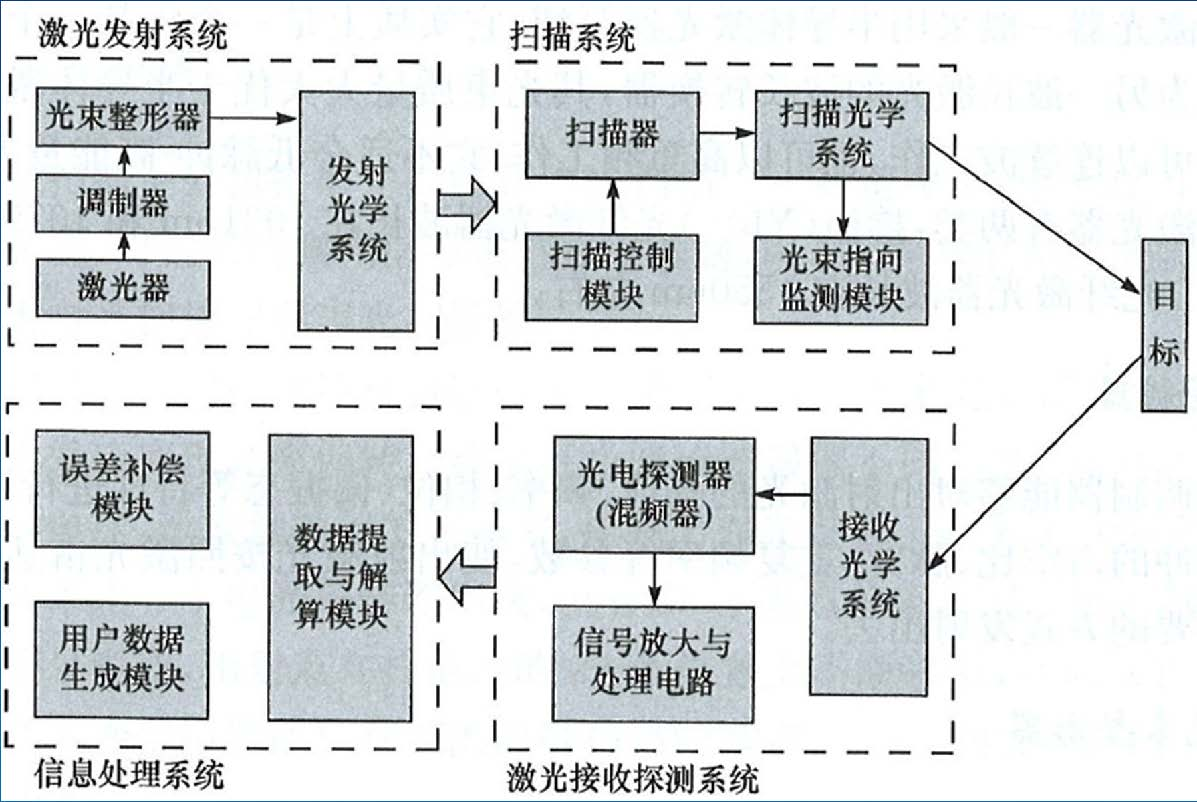
\includegraphics[width=0.7\linewidth]{figure/Chapter1/激光成像雷达的基本结构.jpg}
	\caption{激光成像雷达的基本结构}
	\label{fig:激光成像雷达的基本结构}
\end{figure}
\paragraph{激光成像雷达的发展}
\begin{itemize}
	\item 20世纪70年代,卫星激光测距(阿波罗登月计划)
	\item 1980至1988,机载LiDAR可行性研究。
	\item 1990年,斯图加特大学研制成功首个激光断面测 量系统
	\item 1993年,德国出现首个商用LiDAR系统TopScan(ALTM 1020)
	\item 1995年,全球有5套商用LiDAR系统
	\item 1999年,全球约有30几套商用LiDAR系统
	\item 2001年,全球约有75个公司使用了60几套商用LiDAR系统
	\item 2002年,全球约有120个公司使用了75几套商用LiDAR系统 ,年平均增长率为7.1\%,市场份额从5\%增长到12\%。
	\item 目前国内已引进20余套机载激光雷达系统。
\end{itemize}
\paragraph{激光雷达的新类型}\begin{enumerate}
	\item \textit{扫描激光雷达}\begin{itemize}
		\item 扫描成像激光雷达在对地观测领域最为成熟的应用是机载LiDAR系统。
		\item 采用单元探测器,每次测量只获得一个像素的数据,通过平台运动和扫描实现一定探测范围的成像。
		\item 机载LiDAR系统一般采用脉冲激光体制,要求激光的重复频率高,脉冲宽度窄,单脉冲能量大。
		\item 由记录的距离数据形成的图像称为距离图像,由记录的回波强度数据形成的图像称为强度图像。
	\end{itemize}
	\item \textit{凝视激光雷达(新型)}\\
	\textbf{原理}:凝视成像激光雷达需要控制发射激光,使发射光覆盖整个成像区域,然后通过面阵探测器接收回波,通过飞行时间测量或调制解调手段实现并行测距,得到目标三维图像。\\
	\textbf{优点}:凝视成像激光雷达实现了“瞬时”成像,具有结 构简单、成像速率高、像素分辨率高等诸多优点,有着广阔的应用前景。
	\item \textit{合成孔径激光雷达(新型)}\\
	\textbf{原理}:原理与微波合成孔径雷达类似,不同的是辐射源采用了激光波段。在距离向上发射大时宽带宽信号,对回波信号进行脉冲压缩得到距离向高分辨率;方位向上利用雷达平台与目标之间的相对运动,记录平台不同位置的目标回波信号,经相关的数据处理在空间上合成一个虚拟的大孔径,实现方位向聚焦,获得方位向的高分辨率。\\
	\textbf{优点}:合成孔径激光雷达是一种新型的主动式激光成像 雷达,它综合了传统的微波合成孔径雷达和激光雷达的优势。突破实孔径的衍射极限,当观测距离达到数百公里甚至更远时,它是唯一能够在有限的光学孔径条件下获得厘米级分辨率的光学成像手段。
\end{enumerate}

\subsection{激光雷达的关键技术}
下列四项技术中,前三项属于硬件技术,均已得到不同程度的解决;第四项技术属于软件技术,目前成为最关键的技术。
\begin{enumerate}
	\item \textit{激光发射器}:高功率和高波束质量的辐射源
	\begin{enumerate}
		\item \textit{气体激光器}\\	%% 气体激光器
		\textbf{特点}:\begin{itemize}
			\item 典型的气体激光器为\ce{CO2}
			\item 最早用于激光雷达的激光器之一
			\item 工作波长为10.6 \textmu m,处于大气窗口。
			\item 至今仍广泛用于激光雷达
		\end{itemize}
		\textbf{优点}:\begin{itemize}
			\item 大气传输性能好,效率高。
			\item \ce{CO2}激光雷达易于实现高灵敏度外差探测和三维成像,信息处理技术成熟。
		\end{itemize}
		\textbf{缺点}:\begin{itemize}
			\item 尺寸比较大
			\item 需要低温制冷
		\end{itemize}
		\item \textit{固体激光器}:应用非常广泛的Nd:YAG激光器 \begin{itemize}
			\item 在典型情况下,脉宽10~30 ns,单脉冲能量为100 mJ~1 J,脉冲重复率为10~100 Hz。
			\item 波长1.06 \textmu m的基频辐射YAG激光器可用于研究大气散射。
			\item 波长0.532 \textmu m的2倍频频光可用于海洋勘探。
			\item 波长0.355 \textmu m和0.266 \textmu m的3倍频和4倍频光可用于测污
		\end{itemize}
		\item \textit{半导体二极管激光器},又称半导体激光器又称激光二极管。\\ %% 半导体二极管激光器
		是用半导体材料作为工作物质的激光器。常用工作物质有砷化镓(\ce{GaAs})、硫化镉(\ce{CdS})、 磷化铟(\ce{InP})、硫化锌(\ce{ZnS})等。\\
		激励方式有电 注入、电子束激励和光泵浦三种形式。\\
		\textbf{特点}:半导体二极管激光器是最实用最重要的一类激光器。它体积小、寿命长,并可采用简单的注入电流的方式来泵浦其工作电压和电流与集成电路兼容,因而可与之单片集成。\\
	\end{enumerate}
	\item \textbf{成像探测器}:高灵敏度接收技术。\\ %% 成像探测器
	\textit{成像探测器}也称光电探测器(或混频器),是指将望远镜接收到的激光信号,直接转换成与之对应的电信号,或者将光信号与本振光混频,实现外差探测并将其转换成电信号。\\
	目前激光雷达采用的主流探测器包括:\textit{光电倍增管}(PMT)、\textit{雪崩光电二极管}(APD)、PIN\textit{光电二极管}、\textit{增强型电荷耦合器件}(ICCD)。\\
	激光雷达探测系统所采用的探测器一般有三种类型:\begin{enumerate}
		\item \textit{单元探测器}:\begin{itemize}
			\item 每次只获得一个像素的数据。
			\item 激光器每次发出宽度很窄的脉冲(一般以纳秒计)。
			\item 回波强度反映了目标的反射率特性。
			\item 使用扫描器控制发射脉冲按一定方式扫描,将光束指向不同目标,或目标上的不同位置。
			\item 通过接收系统形成图像,距离数据形成的图像称为距离图像,回波强度数据形成的图像称为强度图像。
			\item 要求激光重复频率高,脉冲宽度窄,单脉冲能量大。
			\item 激光成像雷达的高成像速率和高分辨率常常不能同时得到满足,采用单元探测器时,这一矛盾更加突出,所以需要折中考虑。
		\end{itemize}
		\item \textit{面阵探测器}:\begin{itemize}
			\item 需要控制发射激光,使发射光能覆盖较大面积的目标或同时照射许多不同的目标,然后接收回波信号。
			\item 需要对发射光进行调制,对接收信号进行解调,才能量测出距离。
			\item 不需要扫描器,但要求发射功率大。
			\item 无法采用高灵敏度的探测器。
			\item 在希望成像像素数多,成像速率要求不高的情况下采用。即在成像速率要求不高,成像分辨率要求很高的情况下采取的一种办法。
		\end{itemize}
		\item \textit{阵列探测器}:受限于器件技术以及信号处理技术水平,阵列探测器经历了单元模块阵列化、PIN阵列探测、APD阵列探测,及从线阵到面阵的发展阶段。\begin{itemize}
			\item \textbf{线阵探测}:需要将发射光分为$ N $束,同时照射目标上的$ N $点,从这些点上反射回来的信号由$ N $个探测元所接收,得到$ N $个像素上的距离信息和强度信息;
			\item 通过扫描器扫描,获得二维信息,对扫描器的要求比较高;
			\item 可以实现高速高分辨率成像。
			\item 技术难度较大
		\end{itemize}
	\end{enumerate}
	\item \textbf{扫描系统}:高性能二维扫描技术。用于激光成像雷达系统的扫描器目前可分为三种:力学、电学和二元光学扫描。
	\begin{enumerate}
		\item \textit{力学扫描器}:由反射镜转动或摆动使光束偏转进行大角度范围扫描。结构如图\ref{fig:力学扫描器结构}所示。
		\begin{figure}[htbp]
			\centering
			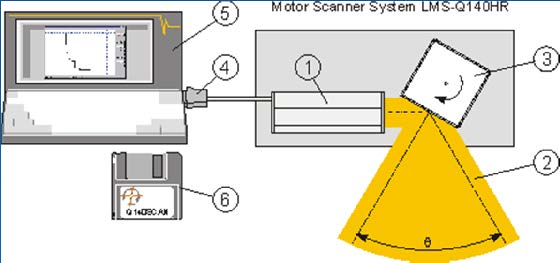
\includegraphics[width=0.7\linewidth]{figure/Chapter1/力学扫描器结构}
			\caption{力学扫描器结构}
			\label{fig:力学扫描器结构}
		\end{figure}\\
			\textbf{优点}:采用转镜可以达到很高的扫描速度,两个转镜可组成二维扫描系统。\\
			\textbf{缺点}:体积较大,笨重,耗电量大。
		\item \textit{声光电学扫描器}:\\
			\textbf{优点}:不包含机械运动,扫描速度快。\\
			\textbf{缺点}:\begin{itemize}
				\item 扫描角度小,一般为几十分之一毫弧度。
				\item 光透过率低,光束质量差。
				\item 耗电量大,光学系统必须作冷却处理。
			\end{itemize}
		\item \textit{二元光学扫描器}:利用二元光学技术制造,通过两组透镜的相对移动实现光束方向的偏转。\\
		\textbf{原理}:利用二元光学技术制造出来的微透镜阵列扫描器由间距只有几微米的微透镜阵列组成,分为两组:一组是正透镜,一组是负透镜。准直光经过透镜时会会聚光,然后通过负透镜时又变为准直光。正透镜阵列和负透镜阵列之间产生相对移动时,准直光的方向就会发生变化。两个微透镜阵列在水平方向相对移动时,输出光束在水平方向就会发生偏转。透镜之间微小的相对移动可以产生几度的光束偏转。\\
		\textbf{优点}:\begin{itemize}
			\item 扫描速度可以达到1KHz以上。
			\item 易于将一束光分为多束光。
			\item 扫描方式可通过编程任意加以改变。
			\item 体积小,重量小。
		\end{itemize}
		\textbf{缺点}:\begin{itemize}
			\item 但扫描角度较小,透过率较低。
			\item 尚未实用。
		\end{itemize}
	\end{enumerate}
	\item \textbf{数据处理技术}:图像处理及目标识别算法
\end{enumerate}

\section{激光遥感集成系统}
\paragraph{激光成像雷达的不足}虽然,激光成像雷达可以获取目标高精度的三维信息(包含高程信息和强度信息),但
\begin{itemize}
	\item 集成GPS/INS方可获取地标目标的绝对位置。
	\item 光谱、纹理信息缺乏,不利于地物识别。
\end{itemize}
\paragraph{激光遥感集成系统}随着数码相机等硬件技术的发展,将数码相机、GPS/INS与激光雷达集成,提高激光雷达的数据获取能力,已成为当前激光雷达系统获取数据的主要方式。(图\ref{fig:激光遥感集成系统})
\begin{figure}[htbp]
	\centering
	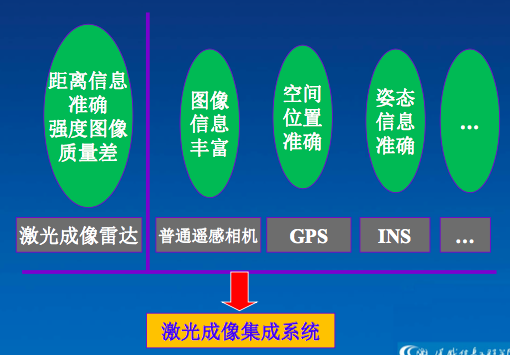
\includegraphics[width=0.7\linewidth]{figure/Chapter1/激光遥感集成系统}
	\caption{激光成像集成系统}
	\label{fig:激光遥感集成系统}
\end{figure}
\paragraph{激光遥感观测系统}由以下部分组成
\begin{itemize}
	\item 飞机
	\item 激光扫描仪
	\item 航摄相机
	\item 导航控制系统
	\item 高精度位置姿态测量系统(IMU/DGPS)
	\item IMU与相机连接架
	\item 机载DGPS天线
	\item 地面DGPS基站接收机
\end{itemize}
\paragraph{激光遥感集成系统的发展}\begin{enumerate}
	\item 美国航空航天局(NASA)最早支持开发激光成像三维测量的机载集成系统。
	\item 加拿大、瑞典、德国以及中国也相继开发出这类机载集成系统,可用于陆地和浅海水下地形测量。
\end{enumerate}
\section{国内常见LiDAR系统的扫描方式}
\paragraph{摆镜扫描}Leica、Optech采用的扫描方式。如图\ref{fig:摆镜扫描方式}所示。
\begin{figure}[htbp]
	\centering
	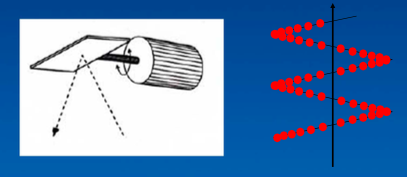
\includegraphics[width=0.7\linewidth]{figure/Chapter1/摆镜扫描方式}
	\caption{摆镜扫描方式图示}
	\label{fig:摆镜扫描方式}
\end{figure}
\paragraph{旋转棱镜扫描}Toposys Harrier、Riegl、IGS采用。如图\ref{fig:旋转棱镜扫描方式}所示。
\begin{figure}[htbp]
	\centering
	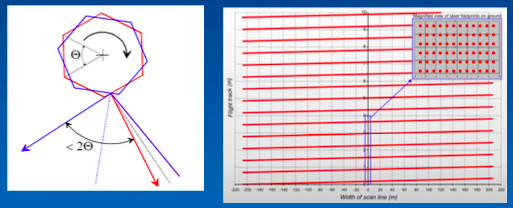
\includegraphics[width=0.7\linewidth]{figure/Chapter1/旋转棱镜扫描方式}
	\caption{旋转棱镜扫描方式}
	\label{fig:旋转棱镜扫描方式}
\end{figure}
\paragraph{光线扫描方式}Toposys Falcon系列。如图\ref{fig:光纤扫描方式}所示。
\begin{figure}[htbp]
	\centering
	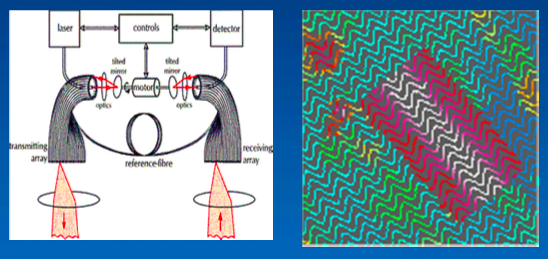
\includegraphics[width=0.7\linewidth]{figure/Chapter1/光纤扫描方式}
	\caption{光纤扫描方式}
	\label{fig:光纤扫描方式}
\end{figure}
\paragraph{圆锥镜扫描方式}opEye MK 系列、国产三维激光成像仪采用。如图\ref{fig:圆锥镜扫描方式}所示。
\begin{figure}[htbp]
	\centering
	\subfloat[圆锥镜扫描原理]{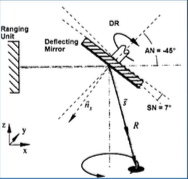
\includegraphics[height=4cm]{figure/Chapter1/圆锥镜扫描_原理}}
	\subfloat[圆锥镜扫描脚点形状]{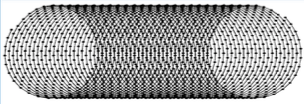
\includegraphics[height=4cm]{figure/Chapter1/圆锥镜扫描_脚点}}
	\caption{圆锥镜扫描方式}。
	\label{fig:圆锥镜扫描方式}
\end{figure}
\section{机载激光三维测量系统对比}
如图\ref{fig:机载激光三维测量系统对比}。
\begin{figure}[!htbp]
	\centering
	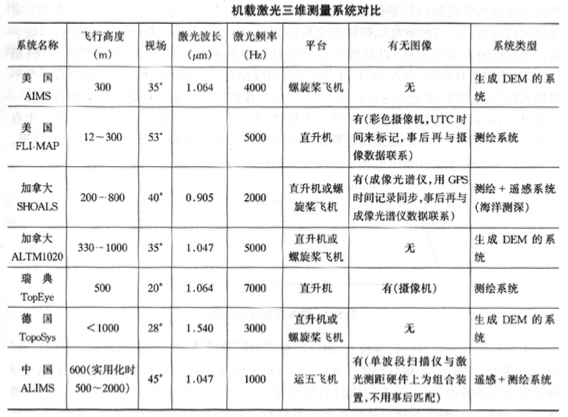
\includegraphics[width=1\linewidth]{figure/Chapter1/机载激光三维测量系统对比}
	\caption{机载激光三维测量系统对比}
	\label{fig:机载激光三维测量系统对比}
\end{figure}

% !TeX root = main.tex
%% Chapter02-激光及激光雷达系统.tex
%% 激光及激光雷达系统
\chapter{激光及激光雷达系统}

\section{激光} %% Section 1 	激光
\textit{激光}(Light Amplification by Stimulated Emission of Radiation, Laser),即“光的手机辐射放大”。

\subsection{辐射与原子} %% Subsection 1.1	辐射与原子
\paragraph{辐射与原子的相互作用的三种过程} \begin{enumerate}
	\item 
		\textit{自发辐射跃迁}:较高能级的粒子,自发地发射一个光子,跃迁到较低能级。其过程如图\ref{fig:自发辐射跃迁}所示。
		\begin{figure}[htbp]
			\centering
			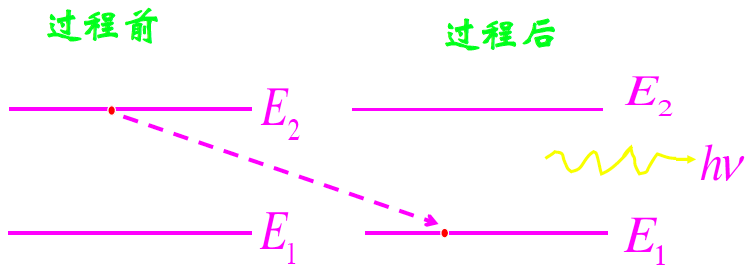
\includegraphics[width=0.7\linewidth]{figure/Chapter2/自发辐射跃迁}
			\caption{自发辐射跃迁}
			\label{fig:自发辐射跃迁}
		\end{figure}
		
		\textbf{光子的频率}为\begin{equation} \nu = \dfrac{E_2-E_1}{h} \end{equation}其中,$ h $是普朗克常量,$ h=6.624 \times 10^{-34} \ \symrm{\mu m} $。
		
		\textbf{自发辐射的速率}为\begin{equation} A_{21} = \dfrac{\diff n_{21}}{\diff t} \dfrac{1}{n_2} \end{equation}
		自发辐射速率的倒数表示由自发辐射所决定的有限寿命\begin{equation} \tau = \dfrac{1}{A_{21}} \end{equation}
		
		具有两个能级的原子系统在外来辐射的作用下可能产生两种过程:\begin{itemize}
			\item 处于低能级E1的原子在外来辐射作用下,吸收一个光子后向高能级E2跃迁(受激吸收过程);
			\item 处于高能级E2的原子在外来辐射作用下,发射一个与入射光子属于同一光子态的光子,并向低能E1级跃迁(受激辐射过程);
		\end{itemize} % 具有两个能级的原子系统在外来辐射的作用下可能产生两种过程
	\item 
		\textit{受激吸收跃迁}:较低能级的粒子吸收一个光子,跃迁到较高能级。其过程如图\ref{fig:受激吸收跃迁}所示。
		\begin{figure}[htbp]
			\centering
			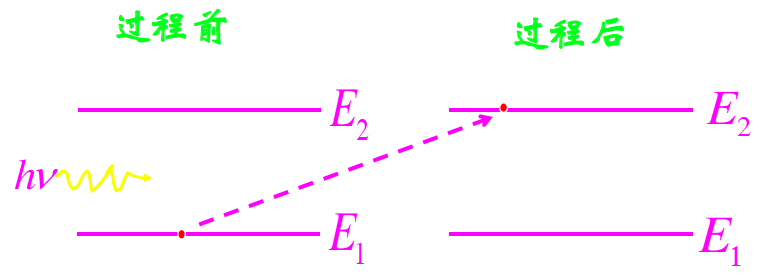
\includegraphics[width=0.7\linewidth]{figure/Chapter2/受激吸收跃迁}
			\caption{受激吸收跃迁}
			\label{fig:受激吸收跃迁}
		\end{figure}
	\item 
		\textit{受激辐射跃迁}:较高能级的粒子在光子激励下跃到较低能级,并发射一个同频率光子。其过程如图\ref{fig:受激辐射跃迁}所示。
		\begin{figure}[htbp]
			\centering
			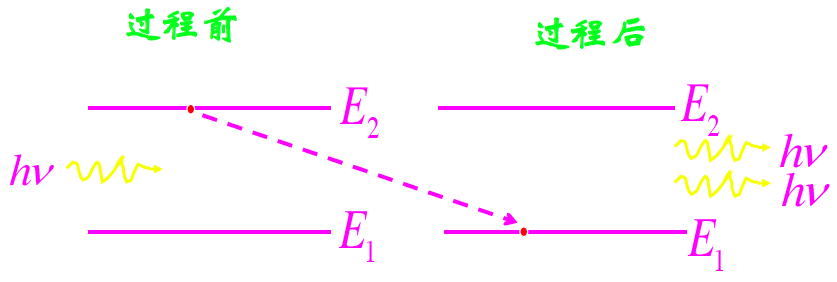
\includegraphics[width=0.7\linewidth]{figure/Chapter2/受激辐射跃迁}
			\caption{受激辐射跃迁}
			\label{fig:受激辐射跃迁}
		\end{figure}
\end{enumerate} % 辐射与原子的相互作用的三种过程

\subsection{受激辐射放大} %% Subsection 1.2	受激辐射放大
\paragraph{外来辐射场的作用}原子系统会产生受激吸收过程和受激辐射过程。\begin{itemize}
	\item \textit{受激吸收过程}:具有一定频率的光子消失的过程,表现为能量由外来辐射场向原子转移,导致辐射场的衰减。
	\item \textit{受激辐射过程}:是原子系统不断产生具有一定频率的光子,表现为能量由原子向辐射场的转移,使辐射场增强。
\end{itemize} % 外来辐射场的作用
一般说来,这两种过程总是同时存在。\begin{itemize}
	\item 如果受激吸收过程占主导地位,最终结果则是辐射场衰减;
	\item 而如果受激辐射过程起主导作用,最终结果就是辐射场的增强。
\end{itemize}% 两种作用同时存在

\paragraph{辐射场增强的条件}在某一段时间$ \diff t $内,由于受激辐射而从能级$ E_1 $向能级$ E_2 $跃迁的原子数为
\begin{equation} \diff n_{12}=n_1W \diff t \end{equation}
由于受激辐射作用而从从能级$ E_2 $向能级$ E_1 $跃迁的原子数为\begin{equation} \diff n_{21}=n_2W \diff t \end{equation}这里假定$ W_{12} = W_{21} = W $。

在两种过程共同作用下,光子的净增量可以表示为
\begin{equation} \Delta N = \left(n_2W - n_1W\right)\diff t = \delta nW\diff t \end{equation}
其中$ \Delta n = n_2-n_1 $。

\textbf{入射光经过原子系统后得到增强的条件}:处于能级E2上的粒子数多于能级E1上粒子数。

根据玻尔兹曼分布定律,处于热平衡状态时,有
\begin{equation} \dfrac{n_2}{n_1} = e^{\frac{E_2-E_1}{kT}} < 1 \end{equation}
即,辐射光通过处于热平衡状态的原子系统时,是辐射场的衰减。

\textbf{粒子反转分布状态}:要使得辐射场得到增强,必须使原子系统的分布为$ n_2>n_1 $。
以某种方式向原子系统提供能量,将足够多的粒子从能级$ E_1 $抽运到$ E_2 $。

\subsection{激光的产生} %% Subsection 1.3	激光的产生
\paragraph{工作物质}原子系统在获得能量后,处于粒子数反转分布状态,称之为\textit{激光工作物质}。工作物质的特点:\begin{itemize}
	\item 工作物质自身某些原子的自发辐射产生的光子, 在传播过程中会作为入射光引起其它原子受激跃迁。
	\item 工作物质处于粒子数反转分布状态,若受激辐射跃迁超过受激吸收跃迁,则光在传播中会得到激励和放大。
	\item 只要工作物质足够长,即使初始信号很小,也会被放大得很强。
\end{itemize}

\paragraph{激光产生的条件}\begin{itemize}
	\item 工作物质处于粒子数反转分布状态。
	\item 受激辐射跃迁超过受激吸收跃迁。
	\item 传播中的光得到激励和放大。
\end{itemize}

\paragraph{激光产生的过程}在工作物质两端分别放置一块反射镜,构成一个\textit{光学谐振腔}。工作物质由抽运系统被抽运到粒子数反转分布状态,因自发辐射而产生的向各个方向传播的光子,在光学谐振腔的作用下,沿着腔轴方向传播的光就会因两端的反射镜往返传播,并很快得到放大。那些传播方向与腔轴方向有一定夹角的光在几次往返后会逸出腔外。由于受激辐射占主导地位,沿腔轴往返传播的光由于受激辐射迅速放大,形成\textit{自激振荡},产生了激光。

受激辐射场与激励场具有相同的频率、相位、传播方向和偏振态,即\textbf{受激辐射光子和激励光子属于同一光子态},所以激光束具有很好的方向性、单色性、相干性。

\begin{figure}[!htbp]
	\centering
	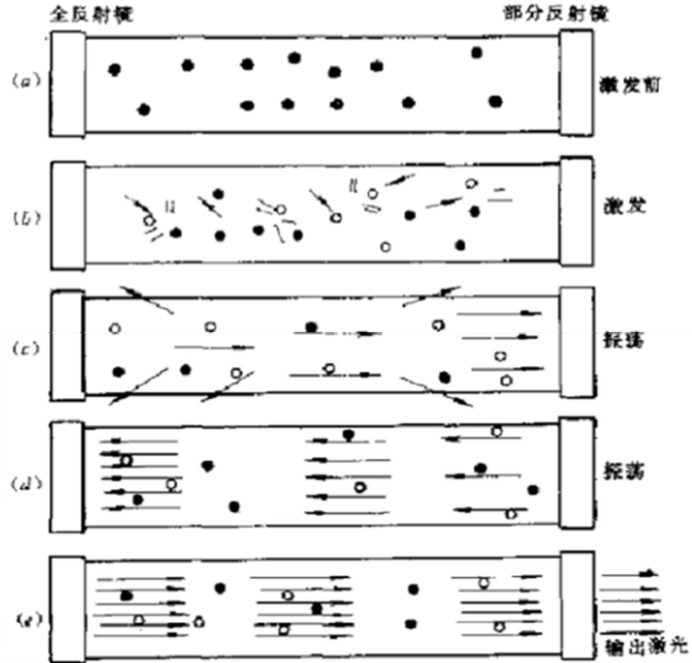
\includegraphics[width=0.6\linewidth]{figure/Chapter2/激光的产生过程}
	\caption{激光产生过程}
	\label{fig:Chpater2-激光产生过程}
\end{figure}

\section{激光器} %% Section 2	激光器

\paragraph{激光器}产生激光的装置称为激光器,激光器虽然多种多样,但其目的都是通过激励和受激辐射放大而获得激光。
\paragraph{激光器的组成}\begin{itemize}
	\item 工作物质
	\item 抽运系统
	\item 光学谐振腔
\end{itemize}
\paragraph{激光器的分类}
\begin{multicols}{2}
	\begin{itemize}
		\item \textbf{按照工作物质分类} 
			\begin{itemize}
				\item 固体激光器
				\item 气体激光器
				\item 液体激光器
				\item 半导体激光器
				\item 自由电子激光器
			\end{itemize} % 按照工作物质分类
		\item \textbf{按转运方式分类}
			\begin{itemize}
				\item 连续激光器
				\item 单次脉冲激光器
				\item 重复脉冲激光器
				\item 锁模激光器
				\item 单模和稳频激光器
				\item 可调谐激光器
			\end{itemize} % 按转运方式分类
		\item \textbf{按激励方式分类}
			\begin{itemize}
				\item 光泵式激光器
				\item 电激励式激光器
				\item 化学激光器
				\item 核泵浦激光器
			\end{itemize} % 按激励方式分类
		\item \textbf{按照输出波段范围分类}
			\begin{itemize}
				\item 远红外激光器
				\item 中红外激光器
				\item 近红外激光器
				\item 可见激光器
				\item 近紫外激光器
				\item 真空紫外激光器
				\item X射线激光器
			\end{itemize} % 按照输出波段范围分类
	\end{itemize}
\end{multicols}

\paragraph{激光的应用}\begin{itemize}
	\item \textbf{自然科学}
	\item \textbf{加工领域}
	\item \textbf{信息处理}
	\item \textbf{激光通信}
	\item \textbf{医学领域}
	\item \textbf{军事领域}
\end{itemize}

\paragraph{未来激光器的发展}
\begin{itemize}
	\item 实用角度
	\item 波长角度
	\item 输出功率
	\item 新类型激光器
\end{itemize}

\subsection{气体激光器} %% Subsection 2.1	气体激光器
\paragraph{用于激光雷达的气体激光器}主要有:\begin{itemize}
	\item \ce{CO2}激光器
	\item \ce{BrHg}激光器
	\item \ce{N2}分子激光器
	\item 准分子激光器
\end{itemize}

工作波长从近紫外到红外;以强放电激励为基本能源。

\paragraph{\ce{CO2}激光器}\ce{CO2}激光器是最早用于激光雷达的激光器之一,工作波长工作波长为10.6 μm,处于大气窗口。至今仍广泛用于激光雷达。

\paragraph{\ce{CO2}分子的震动方式}\ce{CO2}分子的3个原子呈对称排列,震动方式如图\ref{fig:CO2分子的震动方式}所示。
\begin{figure}[htbp]
	\centering
	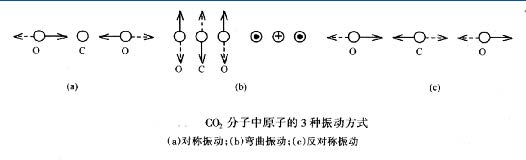
\includegraphics[width=\linewidth]{figure/Chapter2/CO2分子的震动方式}
	\caption{\ce{CO2}分子的震动方式}
	\label{fig:CO2分子的震动方式}
\end{figure}

\paragraph{\ce{CO2}激光器的优点}\begin{itemize}
	\item \ce{CO2}激光器工作波长工作波长为10.6 μm,对人眼安全。
	\item 具有优良的大气传输性能。
	\item 有较大的输出功率和能量转换效率。
	\item 易于进行外差探测。
\end{itemize}

\paragraph{\ce{CO2}激光器的缺点}\begin{itemize}
	\item 需要低温制冷。
	\item 目标对10.6 μm的激光反射率低,且\ce{CO2}激光易被水分子吸收。
\end{itemize}

\paragraph{\ce{CO2}激光器的跃迁机理}
\begin{enumerate}
	\item 
		\textbf{由分子在基态电子能级的振动子能级间跃迁产生}。在放电激励情况下,两种跃迁方式:
		\begin{itemize}
			\item 基态电子能级中(000)振动子能级上的分子与激励电子碰撞,被直接激发到激光能级(001)上,即:
				\begin{equation} \ce{CO2(000) + e\text{(高能)} -> CO2(001) + e\text{(低能)} } \end{equation}
			\item 具有较高的振动子能级分子与其它处于(000)能级上的分子发生碰撞, 跃迁到激光能级(001)。
		\end{itemize}
		两种可能的跃迁方式概率都不大。
	\item 
		\textbf{为了提高跃迁概率,在\ce{CO2}中掺入少量的\ce{N2}气体}。基态电子能级中V=0的振动子能级上的N2分子,被激励电子碰撞后跃迁到V=1的振动能级与CO2的(001)能级接近,很容易将能量转移到处于(000)能级的CO2分子,使它跃迁到(001)能级。即
		\begin{equation} \ce{ CO2(000) + N2(V=1) -> CO2(001) + N2(V=0) } \end{equation}\\
		\textbf{优点}:\ce{N2}分子基态电子能级的V=1子能级寿命相当长,可以积累大量\ce{N2}分子,使较多\ce{CO2}分子从(000)能级跃迁到(001)能级。\\
		\textbf{增加输出功率}:\begin{itemize}
			\item 进一步加入氦气可以使激光输出功率几倍地增大。
			\item 加进适量氙气(\ce{Xe}),也能使其增加输出功率。
			\item 加入适量的水蒸汽(\ce{H2O}),可使激光输出功率显著地增加。
		\end{itemize}
		\textbf{延长激光器的寿命}:在\ce{CO2}激光器里加入氢气(\ce{H2})、一氧化碳(\ce{CO})和氧气(\ce{O2})将延长激光器的寿命。
\end{enumerate}

\subsection{固体激光器} %% Subsection 2.2	固体激光器

\paragraph{常见的固体激光器} Nd:YAG激光器、钛宝石激光器等。

\paragraph{固体激光器的特点}\begin{itemize}
	\item 一般体积较小,与气体激光器相比更加可靠。
	\item 应用十分广泛。
\end{itemize}

\paragraph{Nd:YAG激光器} \begin{itemize}
	\item \textbf{化学组成}:是以钇铝石榴石晶体(化学式是\ce{Y3Al5O15},简称为YAG)为基质,掺入约1\%的激活离子\ce{Nd^3+}就成为Nd:YAG。
	\item \textbf{应用}:用于遥感的Nd:YAG激光器,在典型情况下脉宽10$ \sim $30 ns,单脉冲能量为100 mJ$ \sim $1 J,脉冲重复率为10$ \sim $100 Hz。
		\begin{itemize}
			\item 波长1.06 μm的基频辐射YAG激光器可用于研究大气散射。
			\item 波长0.532 μm的2倍频频光可用于海洋勘探。
			\item 波长0.355 μm和0.266 μm的3倍频和4倍频光可用于测污。
		\end{itemize}
\end{itemize}

\paragraph{二极管泵浦YAG激光器}由于固体激光器在相干性、脉冲重频和输出功率等方面受到局限,遇到CO2 激光器的挑战。寻求新的泵浦方法即二极管泵浦YAG激光器。
\begin{itemize}
	\item \textbf{优点}:泵浦效率高,输出功率高,寿命长。
	\item \textbf{缺点}:结构复杂,成本较高。
\end{itemize}
二极管泵浦Nd:YAG激光器的结构,如图\ref{fig:激光二极管泵浦YAG激光器}所示。
\begin{figure}[htbp]
	\centering
	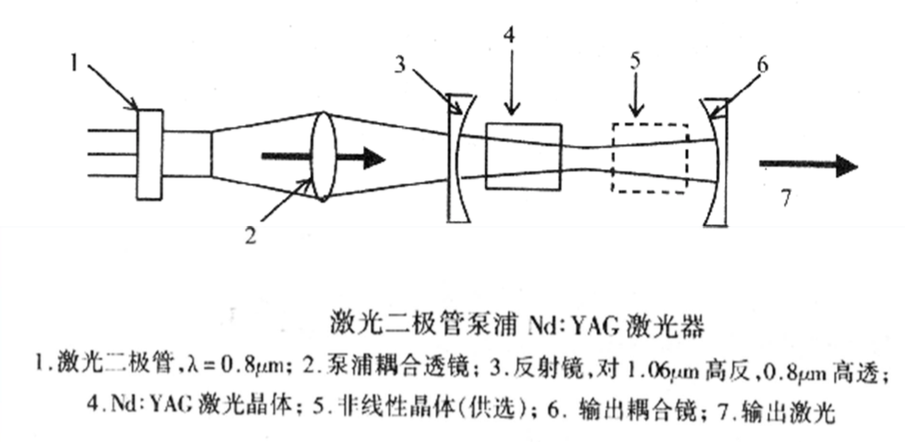
\includegraphics[width=0.7\linewidth]{figure/Chapter2/激光二极管泵浦YAG激光器}
	\caption{二极管泵浦Nd:YAG激光器的结构}
	\label{fig:激光二极管泵浦YAG激光器}
\end{figure}

\paragraph{固体可调谐激光器} 
\begin{itemize}
	\item \textbf{作用}:激光雷达探测对象的响应特性与激光波长密切相关,波长可调的激光器十分有用。
	\item \textbf{类型}:
		\begin{itemize}
			\item 1979年Walling等发明\textit{翠绿宝石激光器}
				\begin{itemize}
					\item 早期有较高实用价值的固体可调谐激光器。
					\item 波长调谐范围是700 $ \sim $ 830 nm。
				\end{itemize} % 翠绿宝石激光器
			\item 1982年Moulton发明\textit{钛宝石激光器}
				\begin{itemize}
					\item 一个重要的进展。
					\item 钛宝石激光晶体的基质是\ce{Al2O3},其中少量的\ce{Al^3+}被\ce{Ti^3+}取代(便于产生激光)。
					\item 钛宝石在400$ \sim $600 nm范围内具有很宽的吸收带,发射带为660$ \sim $1160 nm,波长调谐范围很宽。
					\item 虽然钛宝石具有较大的受激发射截面,增益较高,但激光能级的寿命只有3.2 μs,通常用其它激光器作抽运工作:氩离子激光器、铜蒸气激光器、2倍频Nd:YAG激光器。
				\end{itemize}
		\end{itemize} % 类型
\end{itemize} % 固体可调谐激光器

\subsection{半导体二极管激光器} %% Subsection 2.3	半导体二极管激光器
\paragraph{半导体二极管激光器的特点}
\begin{itemize}
	\item 完全不同的物理机制。
	\item 半导体材料中的电子智能存在于两个能带之一,每个能带所包含的能级数等于晶体中的原子数。根据Pauli不相容原理,每个能级上只能有一个电子。
	\item 半导体材料多是晶体结构。当大量原子规则而紧密地结合成晶体时,晶体中那些价电子都处在晶体能带\footnote{价电子所处的能带称\textit{价带}(对应较低能量)。与价带最近的高能带称\textit{导带},能带之间的空域称为\textit{禁带}}上。本征半导体的能带结构如图\ref{fig:本征半导体能带结构}所示。
		\begin{figure}[htbp]
			\centering
			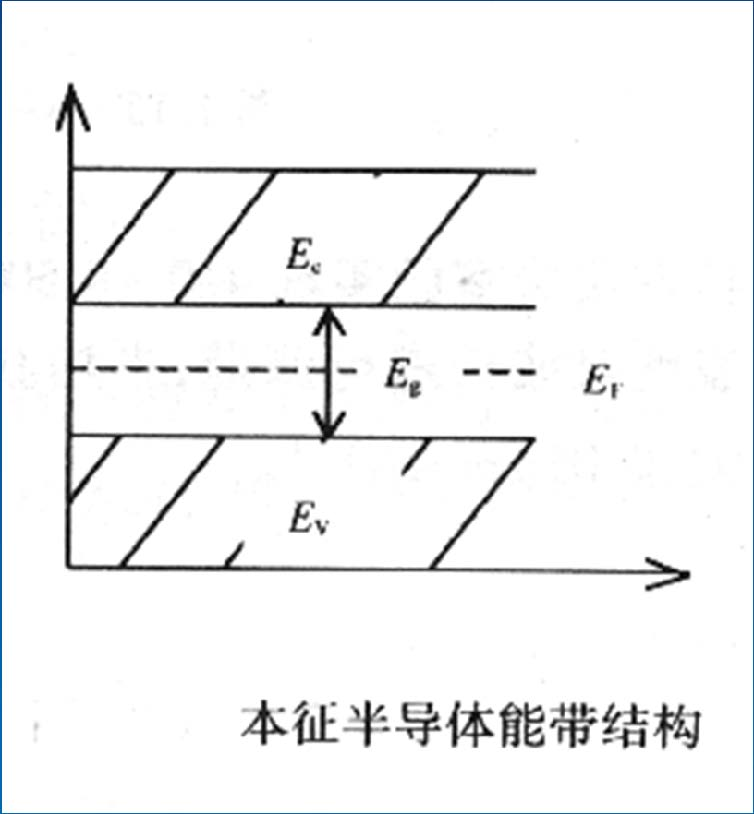
\includegraphics[width=0.3\linewidth]{figure/Chapter2/本征半导体能带结构}
			\caption{本征半导体能带结构}
			\label{fig:本征半导体能带结构}
		\end{figure}
	\item 电子不能再两个能带之间(禁带)驻留。
	\item 没有杂质的纯净半导体,称为本征半导体。
\end{itemize}

\paragraph{半导体二极管激光器的工作原理}
\begin{enumerate}
	\item 如果在本征半导体中掺入杂质原子,则在导带之下和价带之上形成了杂质能级,分别称为施主能级和受主能级。
		有施主能级的半导体称为\textit{n-型半导体};有受主能级的半导体称为\textit{p-型半导体}。
	\item 由于p-半导体与n-半导体所处能级不一致,高低能级的载流子作扩散运动,最终形成\textit{p-n结},此时处于热平衡状态,具有统一的Fermi能级。该过程如图\ref{fig:p-n结}所示。
		\begin{figure}[htbp]
			\centering
			\includegraphics[width=0.5\linewidth]{figure/Chapter2/P-N结}
			\caption{p-n结}
			\label{fig:p-n结}
		\end{figure}
	\item 若加偏压,在结区形成窄区域,导带(高能级)底部能级被电子占据, 价带(低能级)顶部被空穴占据;当导带电子回到价带, 与空穴发生受激复合时就产生了激光。该过程如图\ref{fig:p-n结产生激光}所示。
		\begin{figure}[htbp]
			\centering
			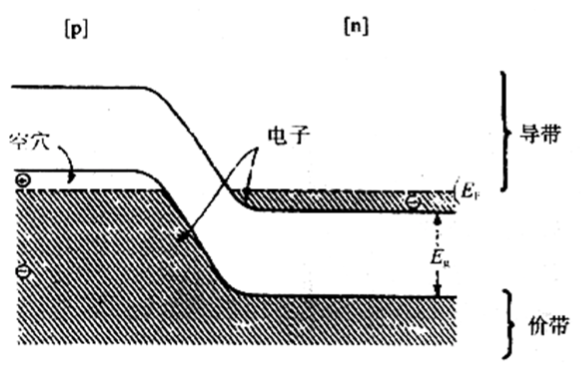
\includegraphics[width=0.5\linewidth]{figure/Chapter2/p-n结产生激光}
			\caption{p-n结产生激光}
			\label{fig:p-n结产生激光}
		\end{figure}
\end{enumerate}

\section{激光雷达系统} % Section 3	激光雷达系统
\subsection{激光雷达系统概述} % SubSection 3.1	激光雷达系统概述

\paragraph{激光雷达的产生}雷达工程师努力探索更短波长的辐射源,在微波振荡器的基础上,发明了激光器,将其与雷达技术相结合,产生了激光雷达技术。

\paragraph{激光雷达的特点}
\begin{itemize}
	\item 角分辨率较高
	\item 距离和速度分辨率高
	\item 抗干扰能力强
	\item 能够与一些目标发生生化作用
	\item 可以对极小的目标进行探测激
\end{itemize}

\paragraph{激光雷达的要求} 激光雷达要求具备发射高功率、窄脉宽、窄频带、较小远场发散角光束较高的脉冲频率的激光器。

\paragraph{激光雷达系统的分类}
\begin{enumerate}
	\item \textbf{按照使用目的分类}
		\begin{itemize}
			\item 探测环境状态
				\begin{itemize}
					\item \textbf{大气}:气溶胶分布、云、气象因素、污染物质……
					\item \textbf{水体}:浮游生物、水温、海洋污染……
					\item \textbf{陆地}:植物生长、热岛效应、污染状况……
				\end{itemize} % 探测环境状态
			\item 量测距离
				\begin{itemize}
					\item \textbf{太空}:星球间距离、星球地形……
					\item \textbf{海洋}:水体深度、水下地形……
					\item \textbf{陆地}:地形图、数字高程模型、植被提取……
				\end{itemize} % 量测距离
		\end{itemize} % 按照使用目的分类
	\item \textbf{按激光和物质的相互作用分类}
		\begin{itemize}
			\item \textbf{反射}:检测比激光波长大很多的物体。地形测绘。
			\item \textbf{米氏散射}:检测微粒直径与激光波长相等的物质。气溶胶。
			\item \textbf{瑞利散射}:检测微粒直径与激光波长小很多的物质。空气分子。
			\item \textbf{拉曼散射}:具有震动和旋转能力的分子。空气分子、水蒸气、\ce{SO2}等污染物质。
			\item \textbf{荧光法}:具有共振能级的分子和原子。\ce{NO2}等污染物质。
		\end{itemize} % 按激光和物质的相互作用分类
	\item \textbf{按使用的激光器分类}
	\item \textbf{按脉冲方式或连续波方式分类}
	\item \textbf{按光波检测的方法分类}
	\item \textbf{按工作台分类}
	\item \textbf{按接收的信号\footnote{激光雷达接收的信号:\begin{itemize}
			\item 可能是反射信号
			\item 也可能是大气散射信号(被称为弹性散射)
			\item 吸收衰减信号、共振散射信号、荧光信号等
	\end{itemize}}分类}
		\begin{itemize}
			\item \textit{反射型激光雷达系统}:地形测绘。
			\item \textit{散射型激光雷达系统}:探测大气中低浓度的尘埃
			\item \textit{吸收性激光雷达系统}:估计某种成分的平均密度
			\item \textit{激光荧光系统}:探测大气中的微量元素
		\end{itemize}
\end{enumerate} % 激光雷达系统的分类

\paragraph{双视场米氏散射激光雷达}武汉大学研制的双视场米氏散射激光雷达,主要由激光发射系统、光学接收系统和信号检测系统组成。

\paragraph{激光雷达系统的结构} 
\begin{itemize}
	\item \textit{双稳系统}:发射部分和接收部分分开放置,目的是为了提高空间分辨率。由于目前脉宽为ns级的激光已达到很高空间分辨率,因此该系统已经很少被采用。双稳系统结构框图如图所示。
		\begin{figure}[htbp]
			\centering
			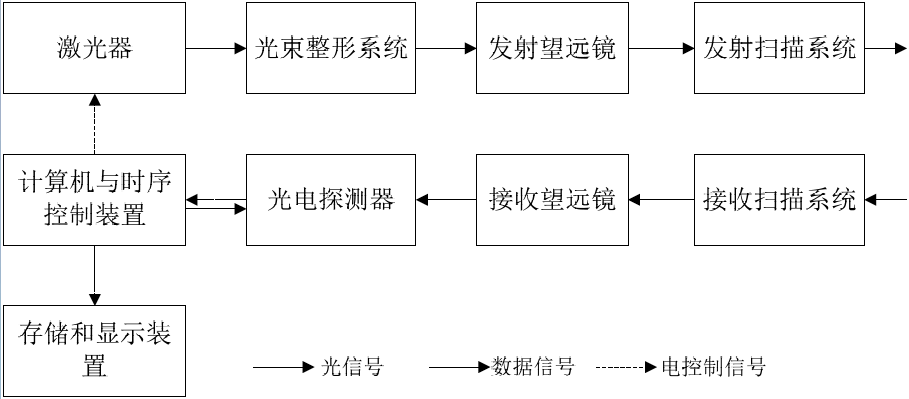
\includegraphics[width=0.7\linewidth]{figure/Chapter2/双稳系统的结构框图}
			\caption{双稳系统的结构框图}
			\label{fig:双稳系统的结构框图}
		\end{figure}
	\item \textit{单稳系统}:发射与接收信号共用一光学子系统,由发送/接收(T/R)开关隔开。单稳系统结构框图如图所示。
		\begin{figure}[htbp]
			\centering
			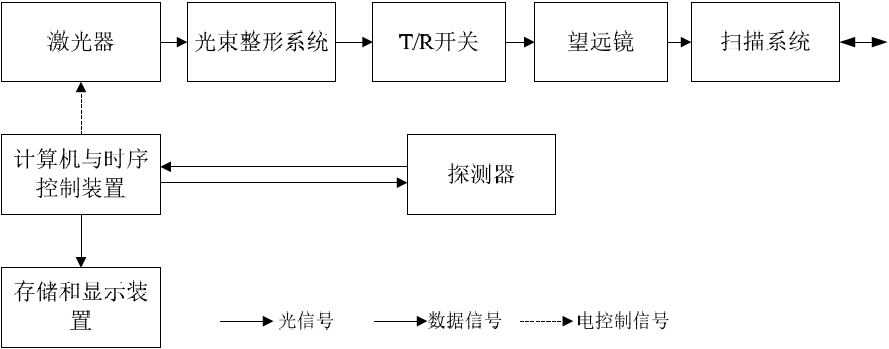
\includegraphics[width=0.7\linewidth]{figure/Chapter2/单稳系统的结构框图}
			\caption{单稳系统的结构框图}
			\label{fig:单稳系统的结构框图}
		\end{figure}
\end{itemize}

\subsection{光束整形} % Subsection 3.2	光束整形

\paragraph{光束整形}通过整形器控制出射激光的指向、方位信息、光束排布状况、束宽等参数,使其形成一定的排布规律,便于检测与分析。

激光器中的光学谐振腔无论是什么形状,其电磁场均具有一定的振荡频率和一定的空间分布,被称为\textit{腔的模式},用$ \mathrm{TEM}_{mn} $表示。其中,$ m = n = 0 $的模称为\textit{基模}。基模场振幅均满足高斯分布,这时激光光束称为\textit{基模高斯光束}。很多情况下要求将基模高斯光束整形为柱状对称,具有平顶强度分布的光束。如图\ref{fig:光束整形}所示。
\begin{figure}[htbp]
	\centering
	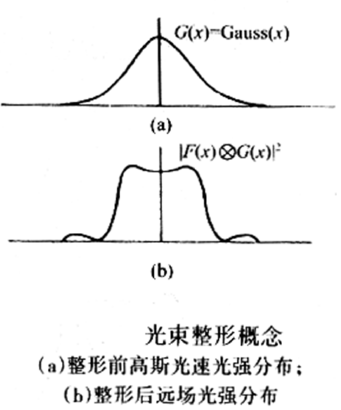
\includegraphics[width=0.3\linewidth]{figure/Chapter2/光束整形}
	\caption{光束整形}
	\label{fig:光束整形}
\end{figure}

\paragraph{光束整形的方法}\textit{衍射光栅}是光束整形的方法之一。光束整形器的能量色散元件由透明二元衍射光栅构成。选择合适的光栅周期和刻线相位调制深度,就可以达到所要求的整形效果。

\subsection{激光扫描} % Subsection 3.3	激光扫描

\paragraph{激光扫描}在光束整形之后,采用某种技术使激光束发生偏转,实现对某区域的目标进行扫描。

\paragraph{激光扫描技术的分类}
\begin{itemize}
	\item \textbf{高惯性扫描}
		\begin{itemize}
			\item 机械技术或反射镜棱镜技术
			\item 主要靠反射镜或棱镜的旋转实现扫描
		\end{itemize} % 高惯性扫描
	\item \textbf{低惯性扫描}
		\begin{itemize}
			\item 电光棱镜的梯度扫描
			\item 振动反射镜的非梯度扫描
			\item 增益控制或损耗控制的内腔式扫描
		\end{itemize}
\end{itemize} % 激光扫描技术的分类

\paragraph{衍射光学元件(DOE)}可替代旋转平面反射镜或棱镜,省去了机械转动部件,减少了折射元件数量,能对任意非球面误差进行校正。如图\ref{fig:衍射光学元件}所示。
\begin{figure}
	\centering
	\subfloat[衍射光学元件的衍射]{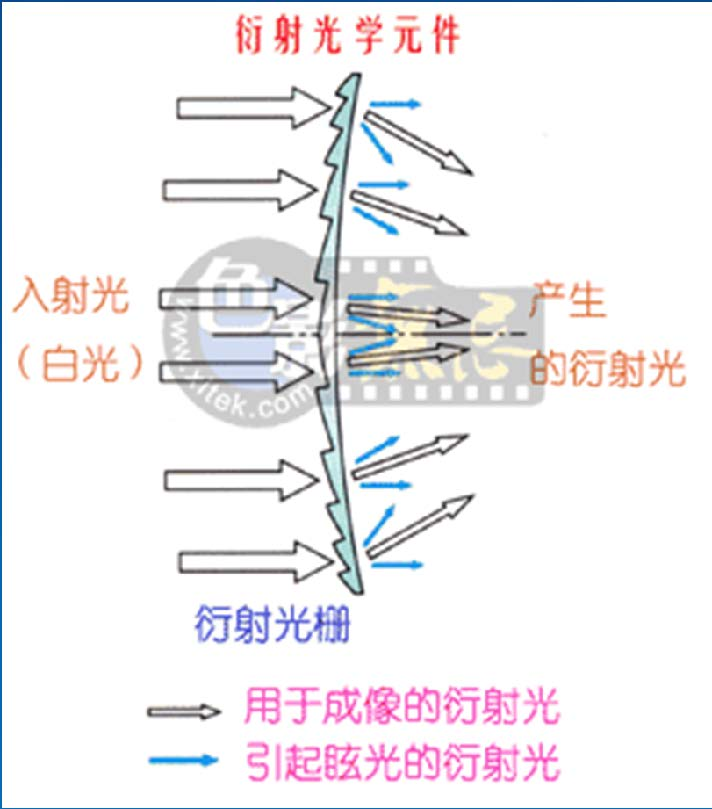
\includegraphics[height=4cm]{figure/Chapter2/衍射光学元件的衍射}}\quad
	\subfloat[DOE物镜后的区场扫描示意图]{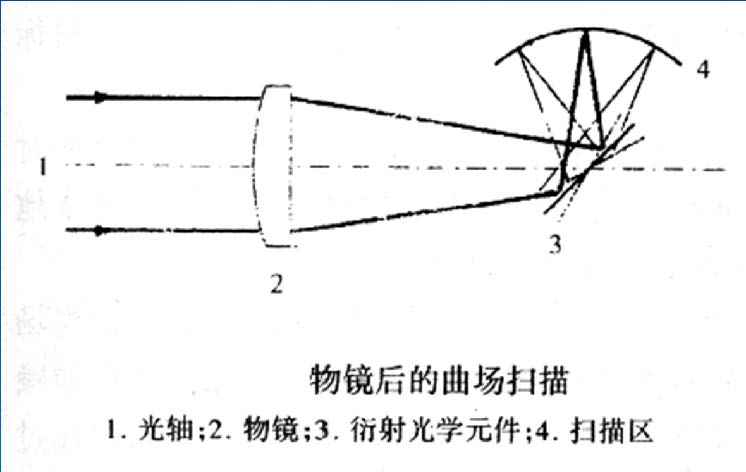
\includegraphics[height=4cm]{figure/Chapter2/DOE物镜后的区场扫描示意图}}
	\caption{衍射光学元件}
	\label{fig:衍射光学元件}
\end{figure}

\subsection{信号接收的探测技术} % Subsection 3.4	信号接收的探测技术
\paragraph{直接探测}将接收到的激光能量聚焦到光敏元件上,产生与入射光功率成正比的电压或电流。与传统的光学接收系统原理基本上相同。
\paragraph{相干探测}探测器接收目标回波信号和某一参考波的相干混合波信号,按照参考波的辐射源及其特性的不同进行探测。分为外差探测,零拍探测和多频外差探测等。
\begin{enumerate}
	\item \textit{外差探测}:
		一般外差探测激光雷达系统由一台连续工作的激光器作为独立辐射源发出参考波,称为\textit{本地振荡器}。
		系统接收到的回波信号与来自本地振荡器的参考信号混合之后,由混频器输出的光束聚焦到探测器上然后再进行信号处理。原理如图\ref{fig:外差探测}所示。
		\begin{figure}[htbp]
			\centering
			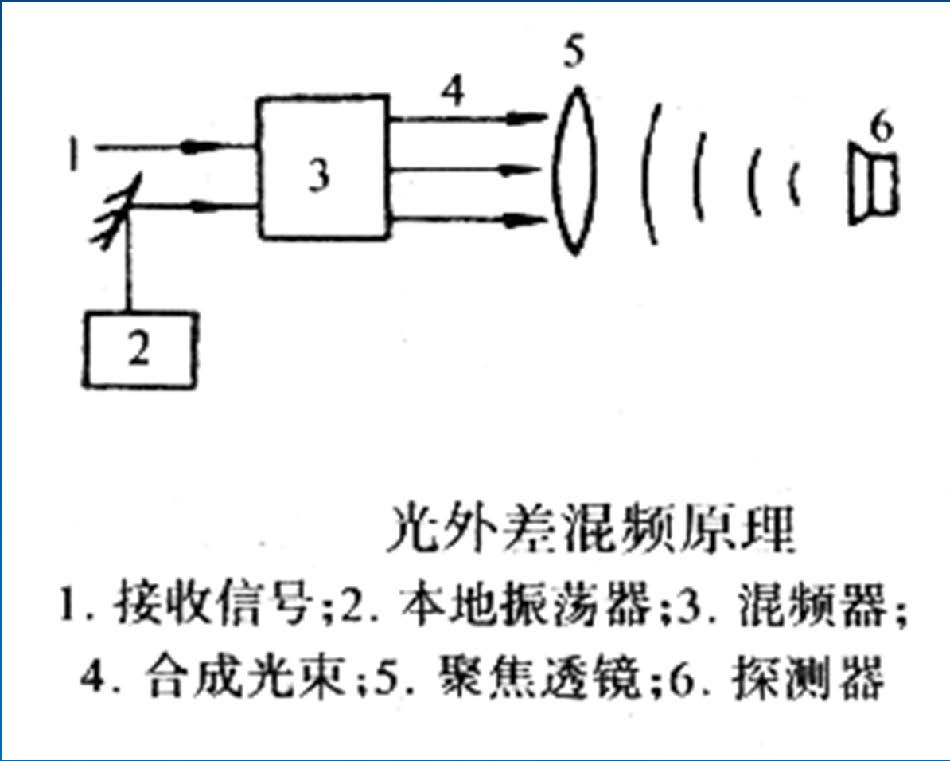
\includegraphics[width=0.5\linewidth]{figure/Chapter2/外差探测}
			\caption{外差探测原理}
			\label{fig:外差探测}
		\end{figure}
	\item \textit{零拍探测}:
		本地振荡信号是来自激光发射源的部分激光辐射,不需要另一个激光源。
		零拍激光雷达比普通外差激光雷达结构更简单,可靠性也更好。
		原理如图所示。
		\begin{figure}[htbp]
			\centering
			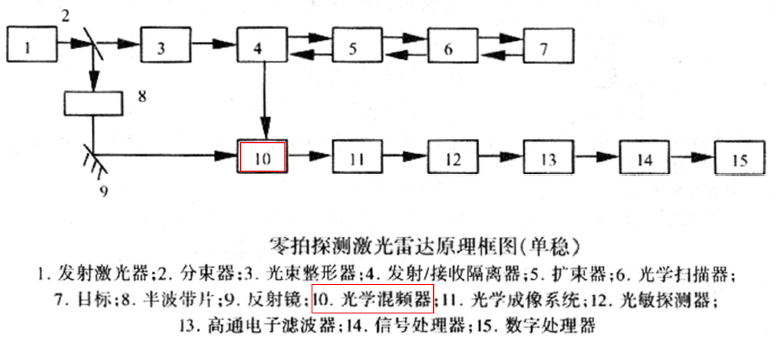
\includegraphics[width=0.7\linewidth]{figure/Chapter2/零拍探测}
			\caption{零拍探测}
			\label{fig:零拍探测}
		\end{figure}
	\item \textit{多频外差探测}:
		目标与激光雷达的相对运动产生接收信号的多普勒(Doppler)频移,可以提供有关目标的非常精确的信息;
		这要求外差探测接收器具有很宽的频带,以覆盖回波信号的频率和外差探测信号频率;
		但增加带宽会提高噪声水平,降低探测概率,解决这一问题的办法是采用三频外差系统。
		
		\textit{三频外差探测}:激光发射有两个独立辐射源,两束激光沿同一光轴向目标传播,经运动目标产生多普勒频移后返回接收器,两个反射信号与本地振荡器信号混频,成像在光敏探测器上。原理如图\ref{fig:三频外差探测系统示意图}所示。
		\begin{figure}[htbp]
			\centering
			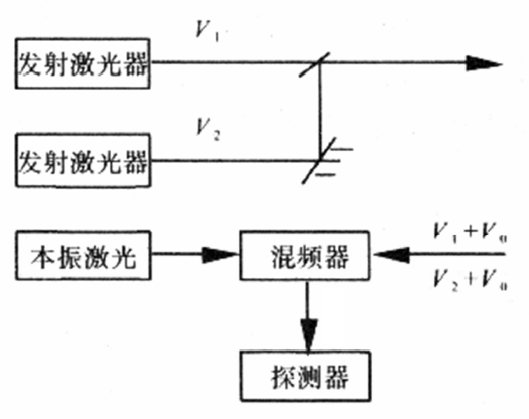
\includegraphics[width=0.5\linewidth]{figure/Chapter2/三频外差探测系统示意图}
			\caption{三频外差探测系统示意图}
			\label{fig:三频外差探测系统示意图}
		\end{figure}
\end{enumerate} % 相干探测的分类

\paragraph{接收孔直径}
\begin{itemize}
	\item 在相干探测激光雷达中,系统的有效接收孔径受散斑现象\footnote{被激光照明的物体,其表面呈现颗粒状结构。}的限制,不能任意扩大。
	\item 当接收孔径小于和等于散斑瓣的平均直径的情况下,接收功率是随接收孔的面积(孔径平方)线性增加;
	\item 在接收孔径增大,大于散斑瓣平均直径的情况下,接收功率不再服从与接收孔径面积线性相关的规律,而是与孔径线性相关;
		这种信号采集效率的下降是接收孔面积增大、反射信号相干性变差的结果;
	
		当接收孔径大于散斑瓣的平均直径时,接收孔有效直径可以表示为
		\begin{equation}
		D = \sqrt{D_rd_s}
		\end{equation}
		其中,$ D_r $表示接收器孔径实际大小,$ d_s $表示散斑瓣直径。
\end{itemize}

\section{激光信号的大气衰减}

\paragraph{激光的大气干扰}两次通过大气,不可避免受到干扰。由于激光光束波长较短,干扰主要有
\begin{itemize}
	\item 大气对它的吸收和散射作用较强,因此大气穿透能力较差。
	\item 大气中雨滴、尘埃、雾、霾等对激光的干扰作用大。
\end{itemize} % 激光的大气干扰

\paragraph{激光大气干扰的表现}
\begin{itemize}
	\item \textbf{衰减}:气体分子和气溶胶粒子、尘埃、雾、雨等的吸收和散射。
	\item \textbf{折射}:由于大气密度分布不均匀,导致激光沿光路产生折射。
	\item \textbf{其他}:大气湍流,导致光束扩展和漂移;大气吸收,引起光束相位变化。
\end{itemize} % 激光大气干扰的表现

\paragraph{激光雷达的性能}
\begin{itemize}
	\item 激光雷达的性能是与激光在大气中的传播特性密切相关的。
	\item 激光的传播特性主要与大气吸收、散射和折射的效应有关。
	\item 要充分发挥激光雷达的效能,就应充分了解激光的大气传播特性,寻找避免或克服大气效应的措施,减少大气衰减,并根据对激光在大气中的传播的规律,仔细选择激光工作波长以及激光工作方式,保证激光光束具有较高的透过率。
\end{itemize}

\subsection{大气衰减效应} % Subsection 4.1	大气衰减效应

\paragraph{布格埃—朗伯特定律}光束传播路径上大气均匀或分层均匀的情况下,目标处的光强可用布格埃—朗伯特定律描述:
\begin{equation}
I(\lambda,z) = I(\lambda,0)e^{-\sigma(\lambda)z}
\end{equation}
式中,$ z $为传播距离,$ I(\lambda,0) $、$ I(\lambda,z) $分别是波长为$ \lambda $的激光光束的初始光强和在距光源$ z $处的光强,$ \sigma(\lambda) $是与波长有关的衰减系数。

\paragraph{大气透过率}当激光束没有出现非线性效应时,大气透过率可以表示为
\begin{equation}
\tau(\lambda) = \exp\left\lbrace -\int_{0}^{L}\sigma(\lambda)\diff r \right\rbrace 
\end{equation}
其中$ L $是传播距离。对于水平平均光程,透过率可以写成
\begin{equation}
\tau(\lambda) = \exp\left\lbrace - \sigma(\lambda)L \right\rbrace
\end{equation}

\paragraph{总的衰减系数}
\begin{equation}
\sigma(\lambda) = \sigma_m + K_m + \sigma_a + k_a
\end{equation}
其中,$ \sigma_m $为分子散射系数,$ K_m $为分子吸收系数,$ \sigma_a $为气溶胶散射系数,$ k_a $为气溶胶吸收系数。
\begin{enumerate}
	\item \textbf{大气分子吸收——吸收系数}
		\begin{enumerate}
			\item \textbf{线吸收}:与单色光波长相应的大气分子的吸收。吸收系数:
				\begin{itemize}
					\item 高度在20 km以内,主要由碰撞压力展宽决定:
						\begin{equation}
						K_{ml} = \dfrac{S}{\pi}\dfrac{r_L}{(v-v_0)^2 + r_L^2}
						\end{equation}
						式中,$ v $是激光的波数,$ v_0 $是激光谱线中心的波数,$ S $为谱线的积分强度,$ r_L $为洛伦兹线半宽度,$ \alpha_D = S \cdot r_D $。
					\item 高度60 km以上,主要由多普勒展宽决定:
						\begin{equation}
						K_{MD} = \dfrac{S}{\alpha_D}\left[\dfrac{\ln 2}{\pi}\right]^{\dfrac{1}{2}} e^{-\frac{\ln 2(v-v_0)^2}{r_D^2}}
						\end{equation}
						式中,$ r_D $是多普勒谱线半宽度,$ \alpha_D = S \cdot r_D $,
						\begin{equation}
						r_d = \dfrac{v_0}{c}\left[\dfrac{2\ln 2k_BT}{M}\right]^{\frac{1}{2}} = 3.58 \times 10^{-7} \left[\dfrac{T}{M}\right] ^ {\frac{1}{2}}
						\end{equation}
					\item 在20$ \sim $60 km高度上,两种形式的吸收同时发生作用。
				\end{itemize} % 线吸收的吸收系数
			\item \textbf{连续吸收}:大气窗口内的大气分子。其吸收特点:
				\begin{itemize}
					\item 是随着光频率连续缓慢变化的分子吸收
					\item 在没有吸收线或只有很弱吸收的波长上,连续吸收成为主要因素
				\end{itemize}
				根据Kneizys得出的水汽连续吸收经验公式:
				\begin{itemize}
					\item 对10.6 μm的\ce{CO2}激光,必须考虑水汽和\ce{CO2}的连续吸收。
					\item 对10.6 μm的YAG激光,其连续吸收可以不加考虑。
				\end{itemize}
				在大气窗口内,水汽的连续吸收必须十分注意的。
		\end{enumerate} % 大气分子吸收——吸收系数
	\item \textbf{大气分子的散射}
		\begin{itemize}
			\item \textbf{瑞利散射}——大气分子。在光的波长远远大于大气中粒子之时, 大气散射表现为瑞利散射,散射系数的经验公式为
				\begin{equation}
				\sigma_m = 2.677 \times 10^{-17} \symrm{PV}^4/\symrm{T}
				\end{equation}
				其中,$ v $为波数。
			\item \textbf{米氏散射}——雨滴、雾滴、霾等粒子。当大气微粒直径很大,与激光波长可比拟之时大气散射服从米氏散射规律,一般说来,米氏散射是气溶胶散射。气溶胶粒子的总衰减系数近似表示:
				\begin{equation}
				\sigma_T = \sigma_a \sigma_m = \dfrac{3.912}{V_M} \left[\dfrac{0.55}{\gamma_{um}}\right]^b
				\end{equation}
				\begin{itemize}
					\item $ V_M $是能见度,即人眼可以辨别目标的最大距离。
					\item $ b $与能见度相关,
						\begin{itemize}
							\item 在一般条件下,$ V_M $为6$ \sim $20 km,$ b=1.3 $。
							\item 能见度特别好,$ V_M > $20 km时,$ b=1.6 $。
							\item 能见度小于6 km时,$ b = 0.585 $。 
						\end{itemize} % b
				\end{itemize} % 米氏散射
		\end{itemize} % 大气分子的散射
		总体说来, 大气分子和气溶胶的散射系数服从高度的负指数规律:随着高度的增加,散射系数很快减小。
		\begin{itemize}
			\item 在5 km以上——气溶胶散射系数与地面相比一般相差一个量级以上。
			\item 接近地面和低空中——气溶胶散射是主要的。
			\item 高空——分子散射与气溶胶散射的效果相当。
		\end{itemize}
\end{enumerate} % 衰减影响因素

\subsection{大气折射效应} % Subsection 4.2	大气折射效应

\paragraph{大气折射效应}激光通过大气时因不同的折射率造成光程增加,传播路径弯曲。

\paragraph{折射率}大气密度随着高度不同而变化,在不同的高度上大气对光的折射率不相同。大气折射率$ n $与激光波长$ \lambda $、空气的温度$ T $、湿度$ e $、压强$ P $有关
\begin{equation}
n = 1 + N(\lambda,T,P,e)
\end{equation}
式中,$ N $为\textit{折射率模数},单位为$ 10^{-6} $,一般简化写成$ N = 0.79 \times \symrm{P/T} $

\section{激光雷达系统能量方程} % Section 5 激光雷达方程

\paragraph{激光雷达方程}激光雷达能量探测的基本数学模型;
激光雷达因与目标作用的机理不同,分为不同的类型,不同类型的激光雷达要用不同的激光雷达方程加以描述。

\paragraph{激光雷达方程的一般形式}
\begin{equation}\label{equ:激光雷达方程的一般形式}
P_r = \dfrac{\eta_o \rho T_a^2 A_r}{\pi R^2} \cdot \dfrac{A_i}{A_b}P_t
\end{equation}
式中,$ P_r $是激光雷达接收到的激光功率;$ P_t $是光学系统效率;$ \rho $是目标表面反射率,$ T_a $是单程大气透过率,$ A_r $是光学系统有效接触面积,$ R $是目标与激光雷达的距离;$ A_i $是目标被照面积(截面积);$ A_b $是目标处的光斑面积。
式\eqref{equ:激光雷达方程的一般形式}\textbf{适用于发射、接收位于同一处的激光雷达的各种应用情况。}

\paragraph{单脉冲稳频激光雷达}探测器所测得的目标,距离探测器$ R $到$ R+\diff R $,辐射源产生的波长间隔为$ [\lambda,\lambda + \diff \lambda] $的微分信号功率为
\begin{equation}
\diff P(\lambda,R) = I(\lambda,R,r)p(\lambda,R,r)\diff\lambda \diff R \diff A(R,r) 
\end{equation}
探测器所接收到的总信号功率则表示为
\begin{equation}
P(\lambda,R) = \int_{0}^{R}\diff R\int_{\Delta\lambda}\int I(\lambda,R,r)p(\lambda,R,r)\diff A(R,r)
\end{equation}
其中,$ p(\lambda,R,r) $取决于
\begin{itemize}
	\item 大气传输因子;
	\item 接收系统传输因子$ T_r(\lambda) $;
	\item 接收立体角$ \dfrac{A_0}{R^2} $;
	\item 接收视场与激光辐射照射面的重叠因子及在距离$ R $到$ R+\diff R $内回波到达探测器的概率$ p(R) $。
\end{itemize} % p(\lambda,R,r)取决于

% !TeX encoding = UTF-8
% !TeX spellcheck = en_US
% !TeX root = main.tex

%% Chapter03-机载LiDAR数据获取基本原理.tex
\chapter{机载LiDAR数据获取基本原理} %% Chapter 机载LiDAR数据获取基本原理

\paragraph{机载LiDAR系统工作原理}如图\ref{fig:机载LiDAR系统工作原理图}所示。
\begin{figure}[htbp]
	\centering
	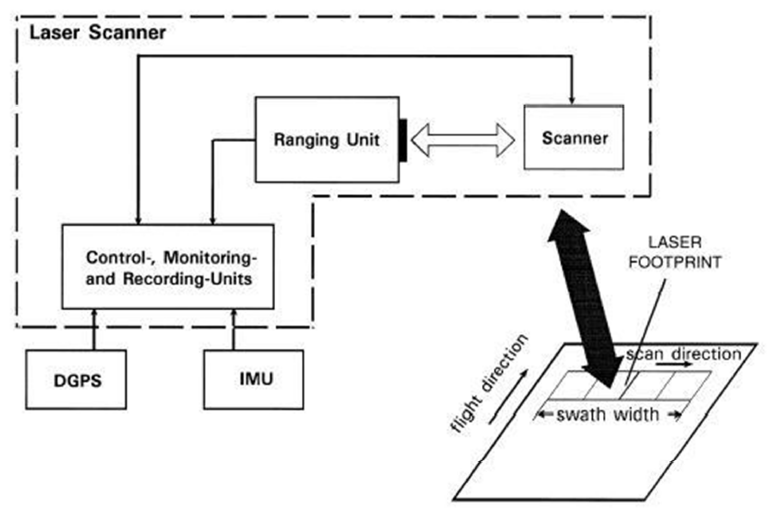
\includegraphics[width=0.7\linewidth]{figure/Chapter3/机载LiDAR系统工作原理图}
	\caption{机载LiDAR系统工作原理图}
	\label{fig:机载LiDAR系统工作原理图}
\end{figure}

图中,
\begin{itemize}
	\item \textit{激光测距单元}包括:激光发射器和接收机。
	\item 光学机械扫描装置:主动工作方式。
		\begin{itemize}
			\item 激光发射器产生激光,由扫描装置控制激光束发射出去的方向
			\item 扫描方向一般与飞机飞行方向垂直。
			\item 扫描宽度由\textit{扫描视场}(FOV,field of view)决定。
		\end{itemize}
	\item 发射和接收激光束的光孔是同一光孔,孔径一般为8$ \sim $15 cm,保证发射光路和接收光路是同一光路。
	\item 发射的激光束是一束很窄的光,发散度很小,形成的\textit{瞬时视场}(IFOV,instantaneons field of view)是由一个很小的角度确定的,一般为0.3 毫弧(mrad)到0.2 毫弧,激光束形成的一个照射角,照射在一小块地面。
	\item 接收机接收被反射回来的激光束后由记录单元进行记录。
\end{itemize}

\paragraph{关键技术}
\begin{itemize}
	\item 激光测距技术
	\item 全球定位系统技术
	\item 惯性测量系统技术
	\item 高性能二维扫描技术
\end{itemize}

\section{激光测距} %% Section	激光测距	========================================
\paragraph{机载LiDAR系统对测距仪的要求}
\begin{itemize}
	\item 精度高
	\item 功率高
	\item 体积小
	\item 波长合适
\end{itemize}

\paragraph{激光测距基本原理}测量激光往返目标所需要时间,然后通过光速$ c $(299792458 m/s)和大气折射系数计算出距离。如图\ref{fig:激光测距基本原理}所示。
\begin{figure}[htbp]
	\centering
	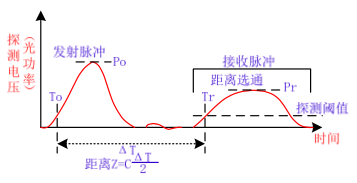
\includegraphics[width=0.7\linewidth]{figure/Chapter3/激光测距基本原理}
	\caption{激光测距基本原理}
	\label{fig:激光测距基本原理}
\end{figure}

\subsection{测距方式} % Subsection	测距方式	----------------------------------------
\paragraph{脉冲测距}
\begin{enumerate}
	\item \textbf{测距原理}:发射脉冲波,测量脉冲信号往返时间差,如图\ref{fig:脉冲测距原理}所示。距离为
		\begin{equation}
		R = \dfrac{1}{2}ct_L
		\end{equation}
		\begin{figure}[htbp]
			\centering
			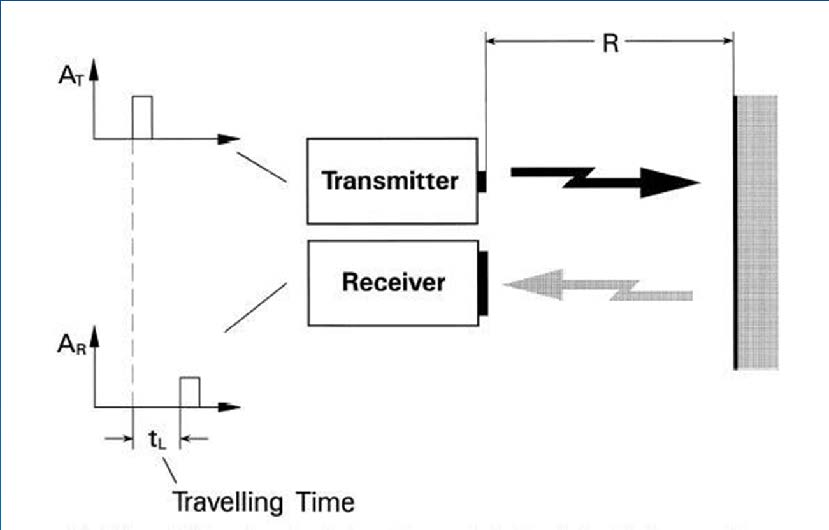
\includegraphics[width=0.5\linewidth]{figure/Chapter3/脉冲测距原理}
			\caption{脉冲测距原理}
			\label{fig:脉冲测距原理}
		\end{figure}
	\item \textit{测距分辨率}:在光束方向能够区分的两个物体的最小距离。
		\begin{equation}
		\Delta R = \dfrac{1}{2}c\Delta t_L
		\end{equation}
		实际上它是取决于$ \Delta t $,即计时器精度。
	\item \textit{最大测量距离}:采用激光器发射激光脉冲时要考虑,避免最远目标所反射的激光束还未返回就发射下一束激光。
	
		需要考虑可能的最大量测距离与最远的目标有关。
		\begin{equation}
		R_{\max} = \dfrac{1}{2}ct_{L_{\max}}
		\end{equation}
		
		\textit{脉冲发射频率}是指一秒钟内能发射多少次激光束,决定了相邻的两束脉冲的时间间隔,由此决定了最大量测距离。
	\item \textbf{脉冲激光测距仪的误差}:对于脉冲激光,计时器主要依脉冲的特殊点进行记录。
		实际脉冲并非一个完全的矩形波,一般事先确定一个阈值,当信号电压到达这一阈值时,计时器即开始记录,由阈值触发器电路控制,结束记录时也是如此。
		
		\textbf{计时误差}:如果所接收的激光幅值很低,电压值未调整到与发射时相同电压值,所记录时间就会过长!解决办法:
			\begin{itemize}
				\item 一般在记时器的前端安置一个放大器进行信号调整。
				\item 为避免因激光幅值变化造成记时错误,采用\textit{分数鉴别器},代替阈值鉴别器: 按信号峰值的比例系数作为记时参照常量。
			\end{itemize}
\end{enumerate} % 脉冲测距

\paragraph{连续波相位差测距}
\begin{enumerate}
	\item \textbf{基本原理}:发射连续波,测量往返连续波的相位差。基本原理如图\ref{fig:连续波相位差测距原理}所示。
		
		\begin{figure}[htbp]
			\centering
			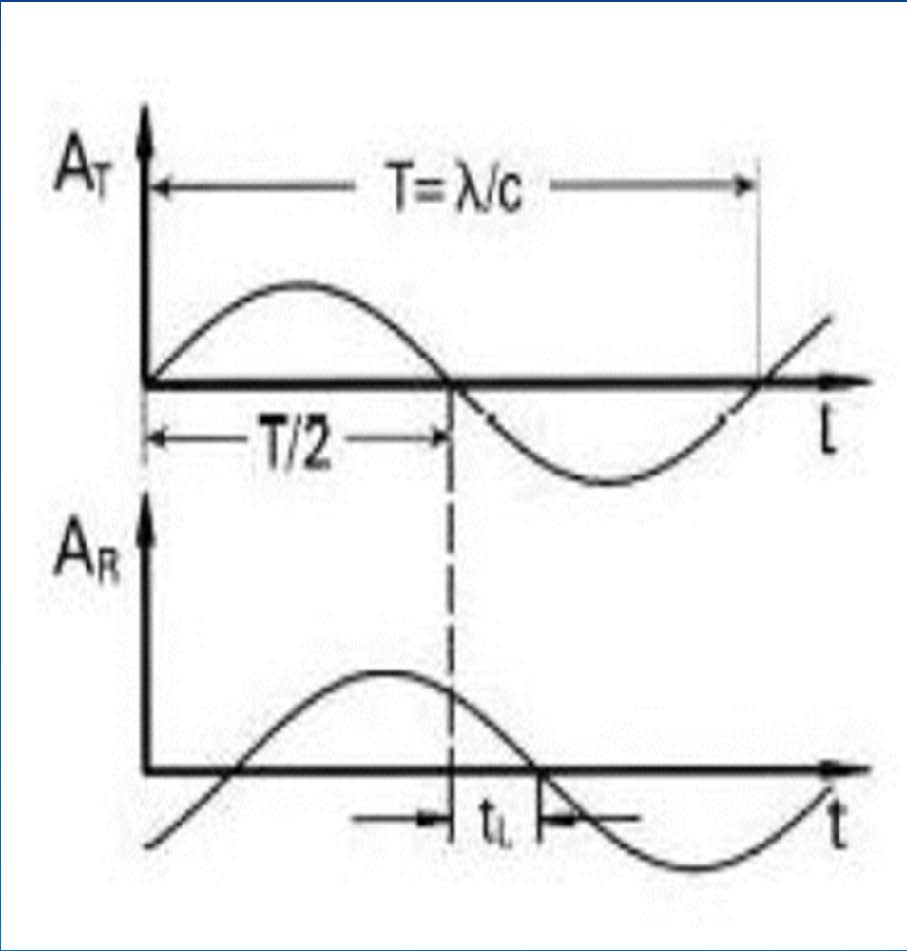
\includegraphics[width=0.5\linewidth,height=0.2\textheight]{figure/Chapter3/连续波相位差测距原理}
			\caption{连续波相位差测距原理}
			\label{fig:连续波相位差测距原理}
		\end{figure}
		
		若在时间$ T $内的被接收的波与被发射波的相位差为$ \varphi $,则从发射到被接收所用时间为
		\begin{equation}
		t_L = \dfrac{\varphi}{2\cpi}\cdot T
		\end{equation}
		
		测量的距离为
		\begin{equation}
		R = \dfrac{1}{2}c \cdot \dfrac{\varphi}{2\cpi}\cdot T = \dfrac{\lambda}{4\cpi}\varphi
		\end{equation}
	
	\item \textbf{测距分辨率}:相位测距中能够准确测量的是一个周期以内的相位差,测距分辨率为
		\begin{equation}
		\Delta R = \dfrac{\lambda_{\text{short}}}{4\cpi}\varphi
		\end{equation}
	\item \textit{整周模糊度}:图中$ t_L $与接收信号与发射信号的相位差成正比。$ t_L $应表示为
		\begin{equation}
		t_L = \dfrac{\varphi}{2\cpi}T+nT
		\end{equation}
		式中,$ n $为激光从发射到接收所走过的距离中的整周数。由于激光波长以微米计,可见$ n $为一个很大的数。由于实际量测的相位差只在之内,实际计算目标到激光器的距离必须计算出整周数$ n $。
	\item \textbf{多测尺频率}:
		若用单一频率测距时是无法确定整周模糊度的值 ,即测距仪存在多值性问题,要解决这一问题,必须采用几个测尺频率测定同一距离。方法:
		\begin{itemize}
			\item 直接多测尺频率:适用于短距离;
			\item 间接多测尺频率:适用于中长距离;
		\end{itemize} % 多测尺频率
	\item \textbf{最大量测距离}:由于相位差的最大量测值为$ 2\cpi $,有
		\begin{equation}
		R_{\max} = \dfrac{1}{4\cpi}\lambda\varphi = \dfrac{\lambda_{\text{long}}}{2}
		\end{equation}
		\begin{itemize}
			\item \textit{最大不模糊距离}:能够准确测量的最大距离,称为最大不模糊距离。
			\item \textbf{双频观测系统}:在采用多频率系统时,由不同频率所对应的波长可兼顾较高的测距分辨率和较大的测量距离。很明显,由最短波长确定了较高的测距分辨率和精度,最长波长确定了最大不模糊距离。
		\end{itemize}
\end{enumerate} % 连续波相位差测距

\paragraph{结论}
\begin{itemize}
	\item 无论是脉冲激光还是连续波激光,在其它条件不变的情况下,最大测距与反射率的平方根和激光功率的平方根成正比。
	\item 要获得较好的测距效果
		\begin{itemize}
			\item \textbf{气候条件}:大气条件十分重要,干、冷和透明的大气条件下,效果最好;
			\item \textbf{时间条件}:夜间最好,最坏的情况是白天阳光强烈;
			\item \textbf{波段选择}:选择大气透过率高的波段;
		\end{itemize}
\end{itemize}

\subsection{测距精度和信噪比} % Subsection	测距精度与信噪比	----------------------------------------
\paragraph{测距精度和信噪比的关系}激光测距系统的测距精度与测距信号的信噪比的平方根成反比,信噪比愈高,测距精度也越高。
\begin{equation}
\sigma \sim \dfrac{1}{\sqrt{S/N}}
\end{equation}

\paragraph{信噪比} 
\begin{itemize}
	\item 信噪比取决于很多因素,如:接收信号功率、信号带宽、背景辐射、探测器响应灵敏度、放大器噪声等。如图\ref{fig:信号参量之间的关系以及对信噪比的影响}所示。
		\begin{figure}
			\centering
			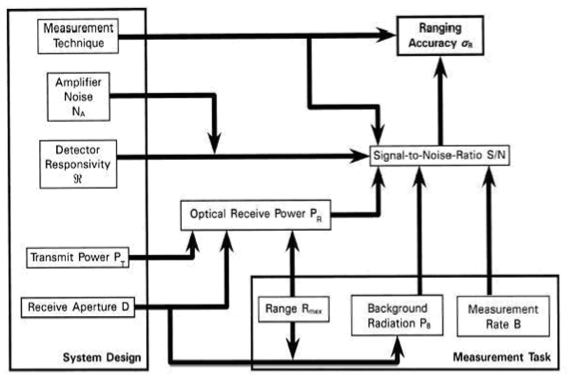
\includegraphics[width=0.7\linewidth]{figure/Chapter3/信号参量之间的关系以及对信噪比的影响}
			\caption{信号参量之间的关系以及对信噪比的影响}
			\label{fig:信号参量之间的关系以及对信噪比的影响}
		\end{figure}
	\item \textbf{信噪比简化}
		\begin{equation}
		S/N = \dfrac{\text{光电二极管电流中的信号功率}}{\text{光电二极管和放大器中的热噪声}}
		\end{equation}
\end{itemize}

\paragraph{两种测距方式的精度}
由于测距精度和信噪比成反比,如果脉冲测距时噪声带宽为$ B_{\text{pulse}} $,相位差测距时噪声带宽为$ B_{\text{cw}} $,则下述关系式成立:
\begin{align}
\sigma_{R_{\text{pulse}}} & \sim \dfrac{c}{2}t_{\text{rise}}\dfrac{\sqrt{B_{\text{pulse}}}}{P_{R_{\text{peak}}}} \\
\sigma_{R_{\text{cw}}} & \sim \dfrac{\lambda_{\text{short}}}{4\cpi}\dfrac{\sqrt{B_{\text{cw}}}}{P_{R_{\text{av}}}}
\end{align}
式中,$ P_{R_{\text{peak}}} $表示脉冲接收功率峰值,$ P_{R_{\text{av}}} $表示连续波接收功率平均值。

假定对同一目标进行量测,可以用发射功率代替接收功率,即以脉冲激光发射功率峰值$ P_{T_{\text{peak}}} $代替接收功率峰值$ P_{R_{\text{peak}}} $,以连续波发射功率平均值$ P_{T_{\text{av}}} $代替接收功率平均值$ P_{R_{\text{av}}} $。于是有:
\begin{equation}\label{equ:两种测距方式精度之比1}
\dfrac{\sigma_{R_{\text{pulse}}}}{\sigma_{R_{\text{cw}}}} \sim 2\cpi \dfrac{c}{\lambda}t_{\text{rise}} \dfrac{P_{T_{\text{av}}}}{P_{T_{\text{peak}}}} \sqrt{\dfrac{B_{\text{pulse}}}{B_{\text{cw}}}}
\end{equation}
假定
\begin{equation}
t_{\text{rise}} \sim \dfrac{1}{B_{\text{pluse}}}
\end{equation}
式\eqref{equ:两种测距方式精度之比1}可以写为
\begin{equation}
\dfrac{\sigma_{R_{\text{pulse}}}}{\sigma_{R_{\text{cw}}}} \sim 2\cpi f \sqrt{\dfrac{t_{\text{rise}}}{B_{\text{cw}}}} \dfrac{P_{T_{\text{av}}}}{P_{T_{\text{peak}}}}
\end{equation}

\paragraph{现状}脉冲激光系统具有大功率、可远距离测距等特点,
目前市场上绝大多数为脉冲激光系统,很少有半导体连续波激光系统。
不过脉冲系统要达到很高的精度需要非常高的技术手段和复杂的处理方法。

\paragraph{测距误差}\textit{测距误差}是指测距仪的显示结果与实际距离之差。
\begin{enumerate}
	\item \textbf{测距误差来源}:噪声、脉冲宽度和幅度、电光系统的延迟以及时间测量单元中基准振荡频率的稳定性。
	\item \textbf{脉冲激光测距仪的误差}
		\begin{itemize}
			\item \textbf{系统误差}:
				\begin{itemize*}
					\item 计数器误差
					\item 大气折射误差
					\item 光电延迟误差
				\end{itemize*}
			\item \textbf{随机误差}:
				\begin{itemize*}
					\item 噪声误差
					\item 距离误差
					\item 漂移误差
				\end{itemize*}
		\end{itemize} % 脉冲激光测距仪的误差
	\item \textbf{连续波激光测距仪测距误差}
		\begin{itemize}
			\item \textbf{固定误差}:
				\begin{itemize*}
					\item 数字测相误差
					\item 幅相误差
					\item 照准误差
				\end{itemize*}
			\item \textbf{比例误差}:
				\begin{itemize*}
					\item 真空光速误差
					\item 大气折射率误差
					\item 测尺频率误差
				\end{itemize*}
		\end{itemize} % 连续波激光测距仪测距误差
	\item \textbf{影响LiDAR测距精度的因素还有}
		\begin{itemize}
			\item 激光功率
			\item 光束发散度
			\item 目标反射特性
			\item 探测器灵敏度
			\item 飞行高度
			\item 飞机姿态
		\end{itemize} % 影响LiDAR测距精度的因素还有
\end{enumerate} % 测距误差

\subsection{功率} % Subsection	功率	----------------------------------------
由于LiDAR系统是在空中对地面进行扫描的,它需要有很高的工作功率,这样才能使激光束的能量尽可能大,经过长距离的大气损耗 和目标吸收等能量损失后,回到探测器时能够有足够的能量,使得探测器能够对光束进行记录。

\paragraph{峰值功率与平均功率}
对于脉冲测距系统,激光能量为:
\begin{equation}
E_{\text{pluse}} = P_{T_{\text{peak}}} t_{\text{pulse}}
\end{equation}
式中,$ t_{\text{pulse}} $为脉冲宽度,$ P_{T_{\text{peak}}} $为发射功率峰值。
	
如果脉冲频率为$ f_{\text{pluse}} $,则平均功率为
\begin{equation}
P_{T_{\text{av}}} = E_{\text{pluse}}f_{\text{pluse}}
\end{equation}

联立求解,得
\begin{equation}
P_{T_{\text{peak}}} = \dfrac{E_{\text{pluse}}}{t_{\text{pulse}}} = \dfrac{P_{T_{\text{av}}}}{t_{\text{pulse}}f_{\text{pluse}}}
\end{equation}
尽管平均功率不大,脉冲激光测距能够产生很高的峰值功率。

\paragraph{发射功率与接受功率}
\begin{equation}
P_r = \rho \dfrac{M^2 A_r}{\cpi R^2} P_T
\end{equation}
式中,$ M $为大气透过率,$ \rho $为目标反射率,$ R $为目标到激光器的距离,$ A_r $为接收光孔截面积。

接受功率的特点:
\begin{itemize}
	\item LiDAR系统接收的功率只是发射功率的很小部分,必须采用非常灵敏的探测器接收信号 。
	\item 接收功率与距离平方成反比
		\begin{itemize}
			\item 激光束刚刚发射出来,由于空中的尘埃或其它的干 扰,会有一部分信号返回接收光路,即使这个部分非常小,也会被灵敏的探测器认为是目标的回波。
			\item 为了避免这种情况,需要采取\textit{近距离消除技术}(close-range suppression techniques)和其它方法。
		\end{itemize}
\end{itemize}

\subsection{体积} % Subsection	体积	----------------------------------------
由于LiDAR系统安装在空中平台上,飞机 的载重量和体积都是有限的,在有限的空间 中需要装载LiDAR设备、操作人员等。
因此,需要将LiDAR设备的体积和重量减小到最小, 这也要求测距仪的体积和重量都很小。

\subsection{波长} % Subsection	波长	----------------------------------------
\paragraph{选择波长的依据}
\begin{itemize}
	\item 大气窗口
	\item 背景光的区别
	\item 目标反射率
	\item 探测器灵敏度
	\item 人眼安全
\end{itemize}

\paragraph{常见LiDAR系统的激光波长} 如表\ref{tab:常见LiDAR系统的激光波长}所示。

\begin{table}[!htbp]
	\centering
	\begin{tabular}{|c|c|}
		\hline
		              系统              &       激光波长       \\ \hline
		\multirow{2}{*}{Leica ALS50II} &  790$ \sim $820  \\ \cline{2-2}
		                               & 1050$ \sim $1060 \\ \hline
		        Optech 3100EA          &       1064       \\ \hline
		      TopoSys FALCON II        &       1560       \\ \hline
		        Riegl LMS-Q560         &       1500       \\ \hline
	\end{tabular}
	\caption{常见LiDAR系统的激光波长}
	\label{tab:常见LiDAR系统的激光波长}
\end{table}

\section{全球定位系统技术} %% Section	全球定位系统技术	========================================
\paragraph{全球定位系统}\textit{全球定位系统}(GPS, Global Position System)是一种利用人造地球卫星进行点位测量导航的技术。
全称是NAVSTAR GPS(NAVigation Satellite Timing And Ranging Global Positioning System)。

\paragraph{GPS定位原理}利用\textbf{测距交会确定点位}。由于用户接受机使用的时钟与卫星星载时钟不可能总是同步,所以除了用户的三维坐标$ (x,y,z) $外,还要引入一个关于卫星与接收机之间的时间差作为未知数$ \delta T $。所以如果想知道解收机所处的位置,至少要能接收到4个卫星的信号。

\paragraph{GPS的组成}
\begin{itemize}
	\item \textbf{空间部分}:GPS卫星星座。如图\ref{fig:GPS星座}所示。
		\begin{itemize}
			\item 由21颗工作卫星和3颗备用卫星组成。
			\item 均匀分布在六个相互夹角为$ 60^{\circ} $的轨道平面内。
			\item GPS卫星用L波段两种频率的无线电波(1575.42 MHz和 1227.6 MHz)向用户发射导航定位信号,同时接收地面发送的导航电文以及调度命令。
		\end{itemize}
		
		\begin{figure}[htbp]
			\centering
			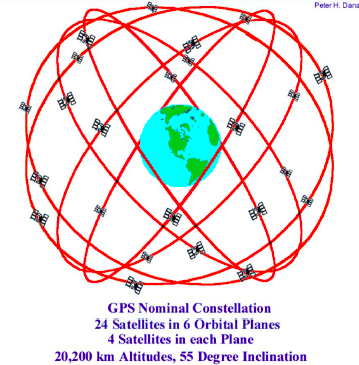
\includegraphics[width=0.5\linewidth]{figure/Chapter3/GPS星座}
			\caption{GPS星座}
			\label{fig:GPS星座}
		\end{figure}
	\item \textbf{地面控制部分}:地面监控系统。
		包括位于美国科罗拉多的主 控站以及分布全球的三个注入站和五个监测站组成,实现对GPS卫星运行的监控。
		主要任务是采集数据(对空中卫星进行连续观测),推算编制各卫星的星历、卫星钟差及大气层的修正参数等,并将这些数据发送到卫星上。
	\item \textbf{用户设备部分}:GPS信号接收机。用来捕获GPS卫星发射的信号,并进行处理,
		根据信号到达接收机的时间,确定接收机到卫星的距离,并最终确定接收机的精确位置。
\end{itemize} %. GPS的组成

\paragraph{GPS的优点}
\begin{itemize}
	\item 观测站之间无需通视
	\item 定位精度高
	\item 操作简便
	\item 全天候作业
	\item 实时定位速度快
	\item 抗干扰性能好,保密性强
\end{itemize}

\paragraph{GPS定位分类}
\begin{enumerate}
	\item \textbf{按定位方式}
		\begin{itemize}
			\item \textit{单点定位(绝对定位)}:采用一台接收机进行定位的模式。只能采用伪距观测量进行概略导航定位,定位精度较差。
			\item \textit{差分定位(相对定位)}:差分GPS(Differential Global Position System,DGPS)
				在用户接收机附近设置一个坐标已知的差分基准站, 连续接收GPS导航信号,将测得的位置或距离数据与已知的位置、距离数据进行比较,
				确定误差,得出改正值,然后将改正数发播给覆盖区域内的用户,用以改正用户的定位结果。
		\end{itemize} % 按定位方式
	\item \textbf{根据定位所采用的观测值} 
		\begin{itemize*}
			\item 测距码伪距GPS定位
			\item 载波相位GPS定位
		\end{itemize*}
	\item \textbf{根据获取定位结果的时间} 
		\begin{itemize*}
			\item 实时GPS定位
			\item 非实时GPS定位
		\end{itemize*}
	\item \textbf{根据定位时接收机的运动状态} 
		\begin{itemize*}
			\item 动态GPS定位
			\item 静态GPS定位
		\end{itemize*}
\end{enumerate}

\paragraph{GPS精度影响因素}
\begin{itemize}
	\item 接收机公有的误差
	\item 传播延迟误差
	\item 接收机固有的误差
\end{itemize}
DGPS技术可以完全消除第一部分误差,大部分消除第二部分误差(取决于基准站和流动站之间的距离)。

\paragraph{LiDAR系统的GPS技术}
LiDAR系统要求很高的定位精度,采取的是载波相位 差分GPS技术,又称为RTK(Real Time Kinematic)技术,
建立在实时处理两个测站的载波相位观测值的基础上,它能实时提供观测点的三维坐标,可以达到厘米级的高精度。

由于涉及到测定遥感器投影中心的位置方位元素,在机载激光雷达系统中,GPS动态定位的精度成为影响系统精度的主要因素。
一般而言,LiDAR系统上使用的载 波相位差分GPS定位精度在5 cm$ \sim $10 cm。

\paragraph{LiDAR系统中GPS的作用}
\begin{itemize}
	\item 确定成像时刻系统中心的地理坐标
	\item 提供相关数据给姿态测量装置,提高测定姿态角的测角精度
	\item 提供导航控制数据
\end{itemize}

\section{惯性测量系统技术} %% Section	全球定位系统技术	========================================
\subsection{惯性导航系统} % Subsection	惯性导航系统	----------------------------------------
\paragraph{基本原理}
\textit{惯性导航系统}(Inertial Navigation System, INS),利用陀螺和加速度计等惯性元件测量运行体在运动过程中的旋转角速度和加速度,计算得到运动体的相对位置、速度和姿态等导航参数。
结构如图\ref{fig:惯性导航系统结构}所示。

\begin{figure}[htbp]
	\centering
	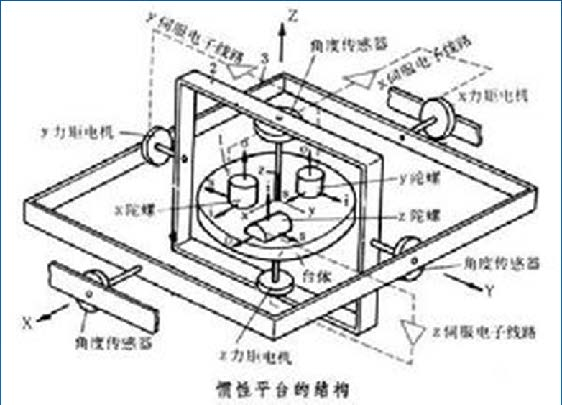
\includegraphics{figure/Chapter3/惯性导航系统结构}
	\caption{惯性导航系统结构}
	\label{fig:惯性导航系统结构}
\end{figure}

\paragraph{作用}可以用于定位、测速、输出姿态信息,以及测定重力异常和垂线偏差、相对大地水准面起伏等。

\paragraph{惯性测量单元} 惯性导航系统中负责姿态测定的陀螺和加速度计等惯性元件总称为\textit{惯性测量单元}(Inertial Measurement Unit, IMU),它是INS的核心部件。IMU通常由三个加速度计和三个陀螺、数字电路和CPU组成的。

\subsection{IMU与DGPS组合定位技术} % Subsection	IMU与DGPS组合定位技术	----------------------------------------
\paragraph{DGPS技术的特点}
\begin{itemize}
	\item \textbf{优点}:使用方便、成本低廉,可量测传感器的位置和速率,高精度、误差不随时间积累。
	\item \textbf{缺点}:动态性能差、数据输出频率低(易受到干扰而失锁),无法量测瞬间的快速变化,没有姿态量测功能等。
\end{itemize}

\paragraph{IMU技术的特点}
\begin{itemize}
	\item \textbf{优点}:姿态量测功能,具有完全自主、无信号传播,既能定位、测速,又可快速量测传感器瞬间的移动,输出姿态信息。
	\item \textbf{缺点}:位误差随着时间迅速积累增长,每次使用前初始对准时间长,不能长时间单独工作,必须不断加以校准。
\end{itemize}

\paragraph{POS系统}GPS技术+IMU技术
\begin{itemize}
	\item 提高了定位精度
	\item 增强了系统可靠性
	\item 部分解决了采样频率低的问题
\end{itemize}

\section{高性能二维扫描技术} %% Section	全球定位系统技术	========================================
\subsection{机载LiDAR系统四种典型的扫描方式} % Subsection	机载LiDAR系统四种典型的扫描方式	----------------------------------------
\begin{enumerate}
	\item \textit{摆镜扫描}:通过电机带动反射镜反复摆动一定的角度,实现激光束在地面的扫描。扫描原理和脚点形状如图\ref{fig:摆镜扫描}所示。
		\begin{figure}[htbp]
			\centering
			\subfloat[摆镜扫描原理]{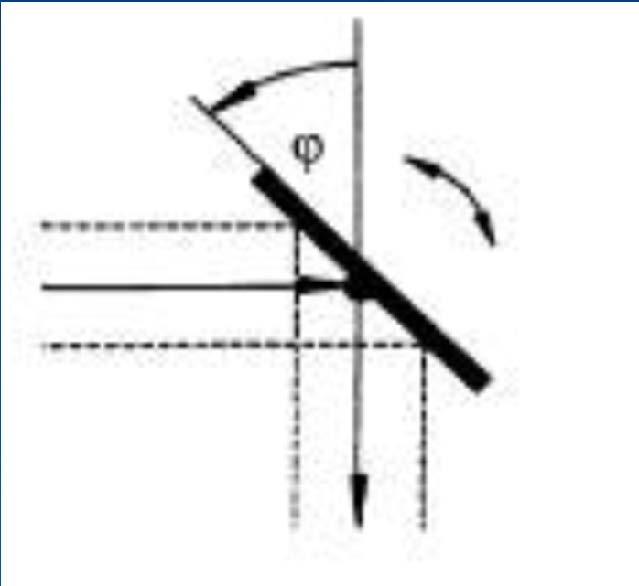
\includegraphics[height=3cm]{figure/Chapter3/摆镜扫描1}}\quad
			\subfloat[摆镜扫描结构]{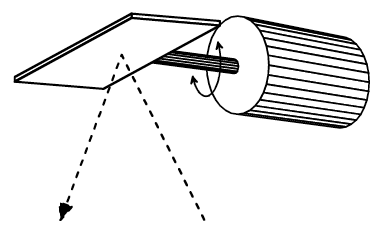
\includegraphics[height=3cm]{figure/Chapter3/摆镜扫描2}}\quad
			\subfloat[摆镜扫描脚点]{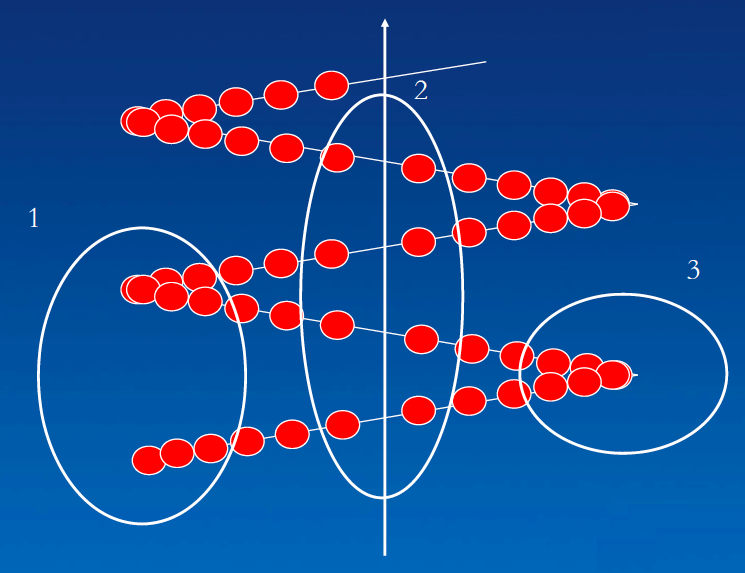
\includegraphics[height=3cm]{figure/Chapter3/摆镜扫描_脚点}}
			\caption{摆镜扫描}
			\label{fig:摆镜扫描}
		\end{figure}
	\item \textit{旋转棱镜扫描}:通过电机带动多面棱镜旋转,由于镜面的位置在不断变化,导致反射光束的方向在一定的范围内往复变化,从而实现激光束在地面的扫描。如图\ref{fig:旋转棱镜扫描}所示。
		\begin{figure}[htbp]
			\centering
			\subfloat[旋转棱镜扫描原理]{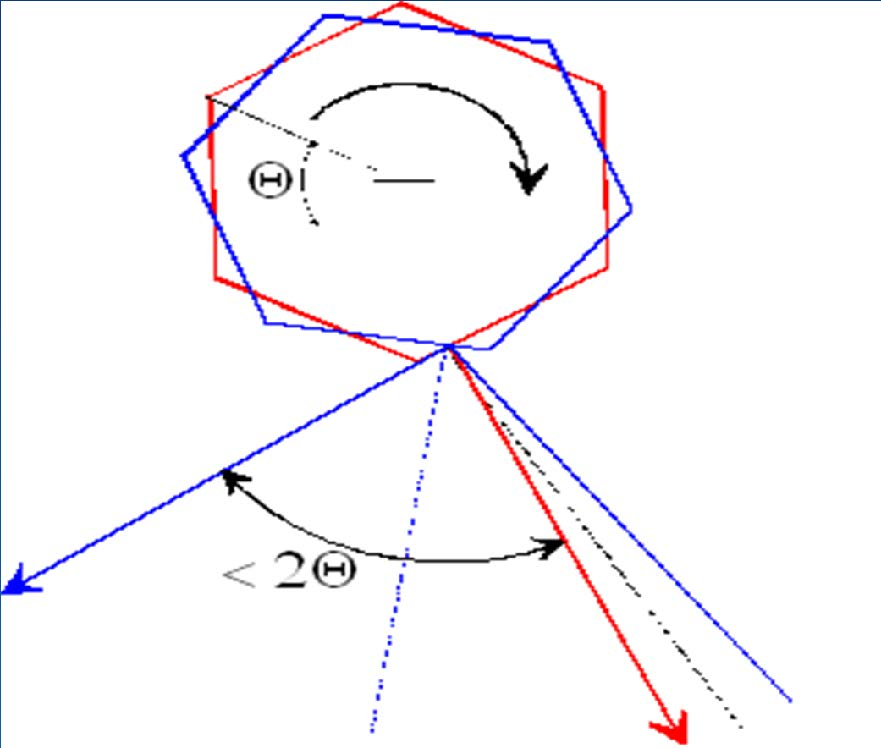
\includegraphics[height=3cm]{figure/Chapter3/旋转棱镜扫描原理}}\quad
			\subfloat[旋转棱镜扫描脚点形状]{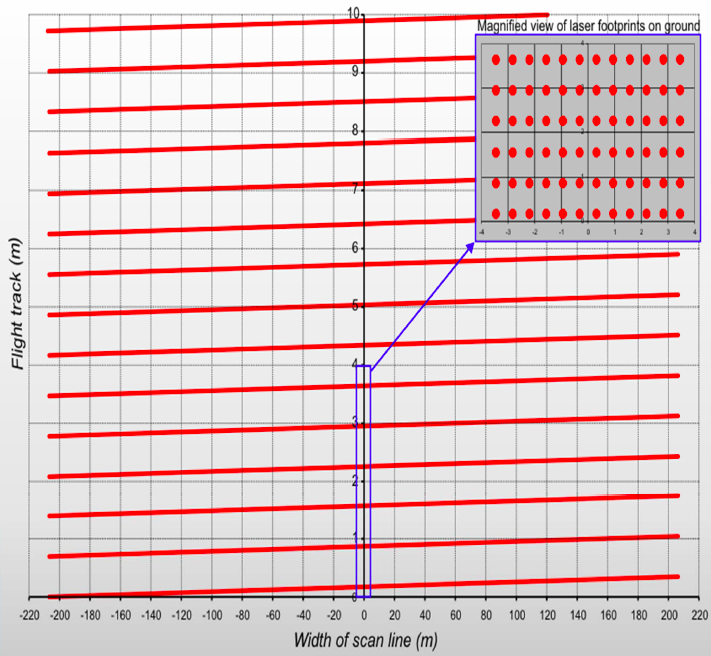
\includegraphics[height=3cm]{figure/Chapter3/旋转棱镜扫描脚点形状}}
			\caption{旋转棱镜扫描}
			\label{fig:旋转棱镜扫描}
		\end{figure}
	\item \textit{椭圆扫描}:旋转一周后在地面形成椭圆扫线。如图\ref{fig:椭圆扫描}所示。
		\begin{figure}[htbp]
			\centering
			\subfloat[椭圆扫描示意图]{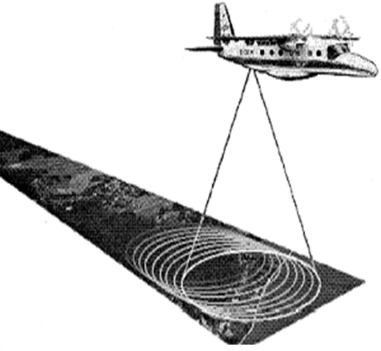
\includegraphics[height=3cm]{figure/Chapter3/椭圆扫描1}}\quad
			\subfloat[椭圆扫描原理]{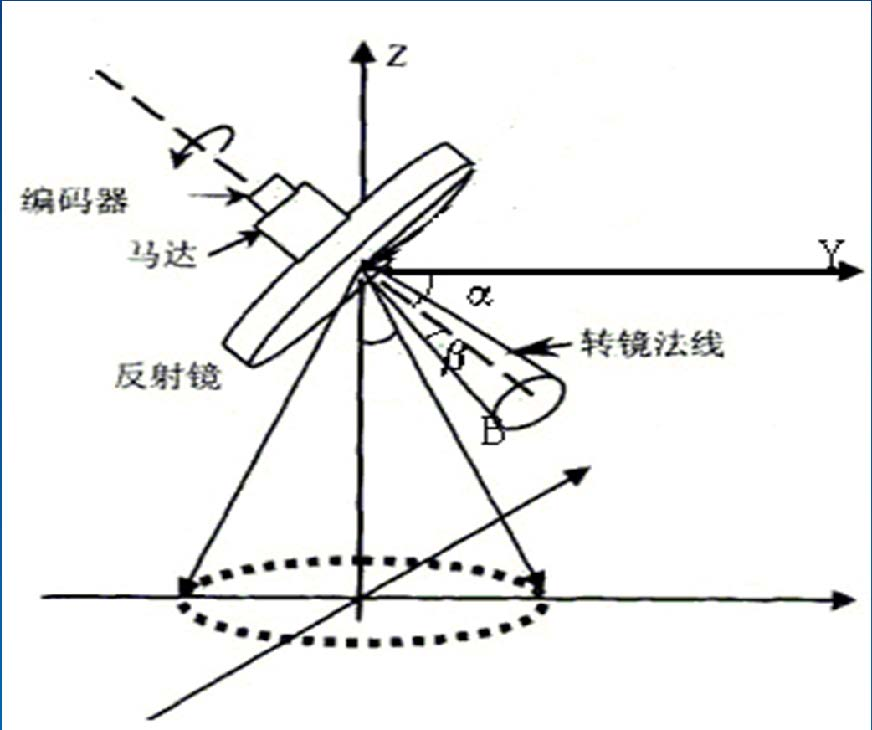
\includegraphics[height=3cm]{figure/Chapter3/椭圆扫描2}}\quad
			\subfloat[椭圆扫描脚点形状]{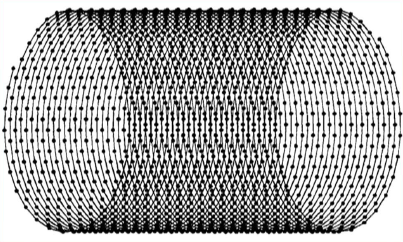
\includegraphics[height=3cm]{figure/Chapter3/椭圆扫描脚点形状}}
			\caption{椭圆扫描}
			\label{fig:椭圆扫描}
		\end{figure}
	\item \textit{光纤扫描}:如图\ref{fig:光纤扫描}所示。目前仅TopoSys激光系统采用光纤扫描仪。目前已有128根光纤组,256根光纤组将可以实现。
		\begin{figure}[htbp]
			\centering
			\subfloat[光纤扫描原理]{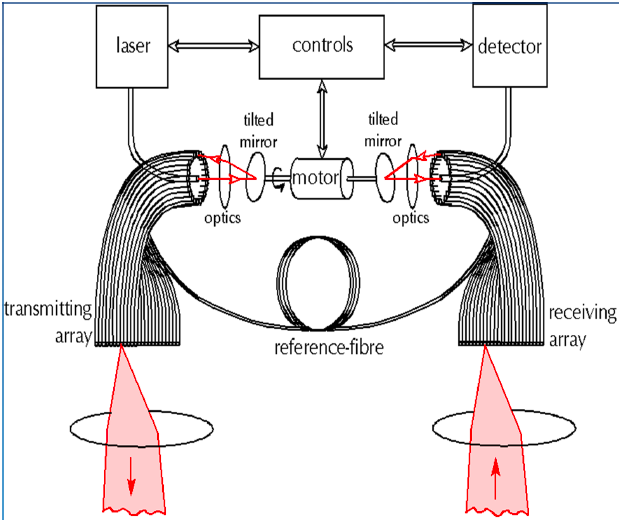
\includegraphics[height=3cm]{figure/Chapter3/光纤扫描原理}}
			\subfloat[光纤扫描脚点]{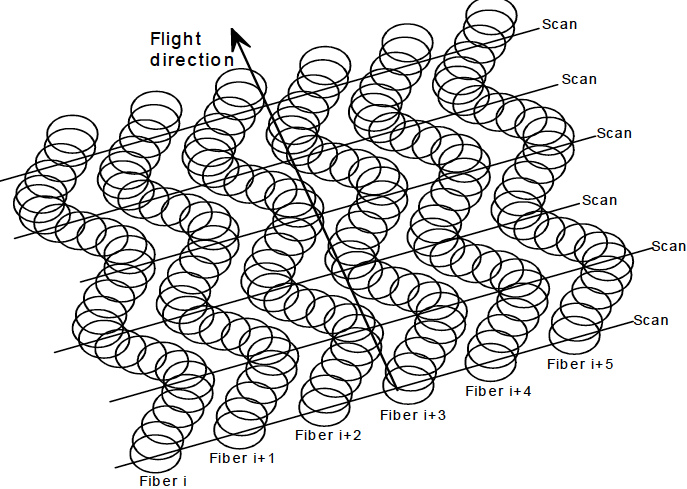
\includegraphics[height=3cm]{figure/Chapter3/光纤扫描脚点}}
			\caption{光纤扫描}
			\label{fig:光纤扫描}
		\end{figure}
\end{enumerate} % 机载LiDAR系统四种典型的扫描方式

\subsection{扫描线形状} % Subsection	扫描线形状	----------------------------------------
扫描线在地面形成的形状不仅取决于激光扫描装置及其工作方式,也取决于飞行方向、飞行速度和地形。

沿着扫描方向对地面目标的连续扫描,是一种等角度步进扫 ,激光所照射的那些点并不是等间距的。由于有时扫 速度不平衡,或加快或减慢,造成扫 线边上的点出现异样,表现出不同的特征,有时就需要从所采集的数据集合中去除这些点。

\paragraph{分类}
\begin{enumerate}
	\item \textbf{按扫描方式}:摆镜扫描;旋转棱镜扫描;椭圆扫描;光纤扫描。
	\item \textbf{按激光扫描方向}:单向扫描;双向扫描。
	\item \textbf{按扫描轨迹}:线扫描;椭圆扫描。
\end{enumerate}

\section{LiDAR数据获取处理}

\paragraph{机载LiDAR获取的数据}
\begin{itemize}
	\item 距离数据、强度信息、CCD等遥感数据
	\item DGPS系统及INS系统等定位定姿数据、航迹文件
	\item 激光点分布模式与技术数据等辅助数据
\end{itemize}
这些信息数据必须通过同步信号,保持相互关联、匹配,才能使用!

\subsection{离线时间同步方案}如图\ref{fig:离线时间同步方案}所示。
\begin{itemize}
	\item POS数据和激光扫描数据存储在不同PC机硬盘中。
	\item POS数据与GPS时间相关,激光扫描数据与PC1的计算机内部时间相关。
	\item PC1与PC2借助GPS的PPS信号关联。
\end{itemize}
\begin{figure}[htbp]
	\centering
	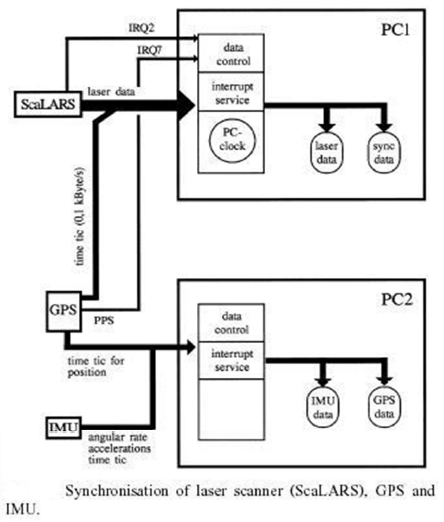
\includegraphics[width=0.5\linewidth]{figure/Chapter3/离线时间同步方案}
	\caption{离线时间同步方案}
	\label{fig:离线时间同步方案}
\end{figure}

\subsection{机载LiDAR系统对地定位方程}

\paragraph{摆镜扫描对地定位方程}通过激光对地面的扫描得到扫描仪与地面上各点的距离,由GPS接收机得到扫描仪的位置,由高精度姿态量测装置量测出扫描仪的姿态,即$ φ $、$ ω $、$ κ $角度,由这些量测值可计算出地面点的三维坐标。

设地面点$ P $在地面坐标系中的坐标为$ (X,Y,Z)_p $, $ P $在传感器坐标系中的坐标为$ (U,V,W)_P $,投影中心$ S $在地面坐标系中的坐标为$ (X_S,Y_S,Z_S) $,传感器的姿态角为$ (\varphi,\omega,\kappa) $,则通用的构象方程为
\begin{equation}
\begin{pmatrix}
X \\ Y \\ Z
\end{pmatrix}_P = \begin{pmatrix}
X_S \\ Y_S \\ Z_S
\end{pmatrix} + \symbf{A} \begin{pmatrix}
U \\ V \\ W
\end{pmatrix}_P
\end{equation}
其中,
\begin{equation}
\symbf{A} = \begin{pmatrix}
a_1 & a_2 & a_3 \\
b_1 & b_2 & b_3 \\
c_1 & c_2 & c_3 
\end{pmatrix}
\end{equation}
是传感器坐标系相对于地面坐标系的旋转矩阵,是传感器姿态角的函数。

对于每一个脉冲,有
\begin{align}
	\begin{split}
	x & = 0 \\
	y & = S \sin \theta \\
	z & = S \cos \theta
	\end{split}
\end{align}
式中,$ \theta $是扫描线方向与$ Z $轴夹角,由编码器按固定的激光脉冲间隔给出;$ S $是激光测距。

代入构像方程,有扫描线定位方程
\begin{equation}
\begin{pmatrix}
X \\ Y \\ Z
\end{pmatrix}_P = \begin{pmatrix}
X_S \\ Y_S \\ Z_S
\end{pmatrix} + \symbf{A} \begin{pmatrix}
0 \\ S\sin\theta \\ S\cos\theta
\end{pmatrix}_P
\end{equation}

\paragraph{椭圆扫描定位方程}
\begin{equation}
\begin{pmatrix}
X_P \\ Y_P \\ Z_P
\end{pmatrix} = \begin{pmatrix}
X_G \\ Y_G \\ Z_G
\end{pmatrix} + \symbf{A} \begin{pmatrix}
-S\sin 2\delta \sin \gamma \\ 
S \cos 2\delta \\ 
-S \sin 2\delta \cos \gamma
\end{pmatrix}
\end{equation}

\section{机载LiDAR数据获取新技术} %% Section	全球定位系统技术	========================================
\paragraph{数字化全波形技术}如图\ref{fig:数字化全波形技术}所示。
\begin{figure}[htbp]
	\centering
	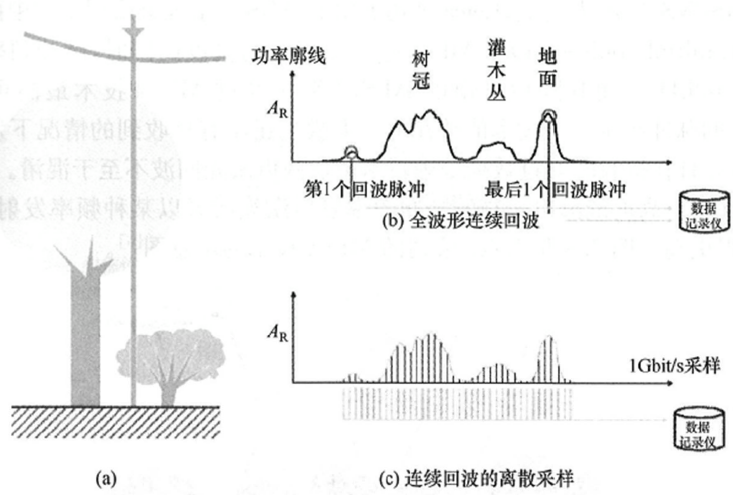
\includegraphics[width=0.7\linewidth]{figure/Chapter3/数字化全波形技术}
	\caption{数字化全波形技术}
	\label{fig:数字化全波形技术}
\end{figure}

\paragraph{空中内插多脉冲技术}如图\ref{fig:空中内插多脉冲技术}所示。
\begin{figure}[htbp]
	\centering
	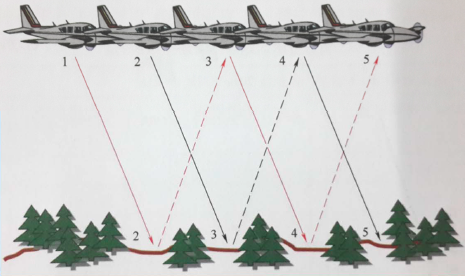
\includegraphics[width=0.7\linewidth]{figure/Chapter3/空中内插多脉冲技术}
	\caption{空中内插多脉冲技术}
	\label{fig:空中内插多脉冲技术}
\end{figure}

\paragraph{双扫描仪组合技术}如图\ref{fig:双扫描仪组合技术}所示。
增加地面激光脚点密度的方法:
\begin{itemize}
	\item 直接的方法就是增大激光脉冲的重复频率和扫描仪的扫描频率。
	\item 多脉冲技术可以通过增加激光脉冲的重复频率来达到这个目的,但是扫描仪的扫描频率由于各方面的限制很难有大幅度的提升。
	\item 双激光雷达组合的系统便应运而生。通过搭载两个激光扫描仪,并使其同时工作,可显著提高地面激光脚点密度。
\end{itemize}

\begin{figure}[htbp]
	\centering
	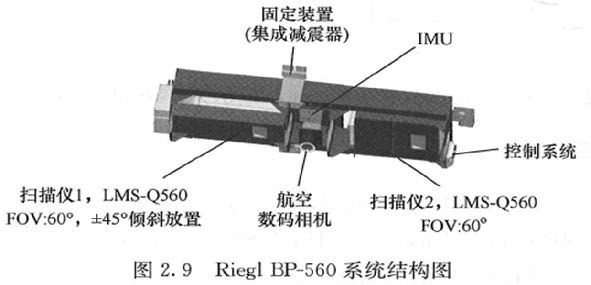
\includegraphics[width=0.7\linewidth]{figure/Chapter3/双扫描仪组合技术}
	\caption{双扫描仪组合技术}
	\label{fig:双扫描仪组合技术}
\end{figure}
% !TeX root = main.tex
% !TeX encoding = UTF-8
% !TeX spellcheck = <none>
%% Chapter03-机载LiDAR数据获取基本原理.tex

\chapter{机载LiDAR数据获取基本原理} %% Chapter 机载LiDAR数据获取基本原理

\section{数据获取重要参数}  %% Section	数据获取重要参数	========================================
\subsection{LiDAR数据获取重要参数的作用}
\begin{itemize}
	\item 与LiDAR系统性能、数据质量相关的参数关系式或计算公式。
	\item 是进行激光遥感系统选择及航线设计的重要依据!
\end{itemize}

\subsection{参数类型}

%p
\kaiparagraph{瞬时视场角(instantaneous field of view, IFOV)} 又称\textit{激光发散角},是指激光束发射时其发散的角度。瞬时视场角的大小取决于激光的衍射(diffraction),是发射孔径$ D $和激光波长$ λ $的函数:
\begin{equation}
\text{IFOV} = 2.44 \dfrac{\lambda}{D}
\end{equation}

%p
\kaiparagraph{视场角(Field Of View, FOV)} 激光束的扫描角,指激光束通过扫描装置所能达到的最大角度范围。

早期LiDAR系统的扫描角一般较小,大约在$ 30^{\circ} $,目前比较先进的LiDAR系统的扫描角都在$ 60^{\circ} \sim 75^{\circ} $度左右,基本能够达到航摄像机的视场角度范围。

%p
\kaiparagraph{脉冲频率}单位时间内激光器所能够发射的激光束数量。

\textbf{注意}:并不是脉冲频率越大越好,过于密集的激光脚点会带来大量的冗余数据,影响数据处理的效率和效果。

%p
\kaiparagraph{扫描频率} 扫描频率指线扫描方式,每秒钟所扫描的行数,即扫描镜每秒钟摆动的周期。很明显,扫描频率越大,每秒钟的扫描线就越多。

%p
\kaiparagraph{垂直分辨率}脉冲通过的路径上所能够区分不同目标间的最小距离。
\begin{equation}
H_{\min} = c \dfrac{t_{\min}}{2}
\end{equation}
若脉冲宽度为10 ns,则在一个脉冲宽度内,不同目标距离至少为1.5 m,其回波能量才可能经接收器检出,并区别开来。

%p
\kaiparagraph{最大飞行高度(最大量测距离)}系统所能精确测定的最远距离。

在实际中工程中,其影响因素有很多:激光功率、光束的发散性、大气折射率、地物反射率、探测器灵敏度等等。

%p
\kaiparagraph{最小飞行高度}取决于
\begin{itemize*}
	\item 飞行平台的类型
	\item 探测地区的地形
	\item 人眼的安全距离
\end{itemize*}

%p
\kaiparagraph{激光脚点光斑特性}包含三个方面:
\begin{enumerate}
	\item \textit{激光脚点光斑直径(激光束照射面直径)}:
		地面上瞬时激光脚点投射在地面上为一个椭圆形的光斑,其航向直径(航线方向,短轴)与旁向直径(扫描方向,长轴)是不等的;
		它们与下列因素有关:平台的飞行高度$ H $;激光波束发散角$ γ $;地形坡度$ α $;瞬时扫描角$ θ_i $。关系如图所示。
		
		\begin{figure}[htbp]
			\centering
			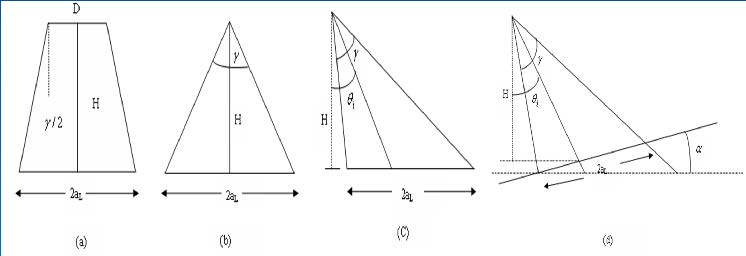
\includegraphics[width=\linewidth]{figure/Chapter4/激光脚点直径}
			\caption{激光脚点直径}
			\label{fig:激光脚点直径}
		\end{figure}
		
		\begin{enumerate}
			\item 当遥感平台处于水平状态,激光束垂直照射水平地面上(瞬时扫描角$ θ_i=0 $)时(图\ref{fig:激光脚点直径}-a),激光脚点光斑的旁向直径
				\begin{equation}
				2a_L = D + 2H \tan \dfrac{\gamma}{2}
				\end{equation}
				通常探测器孔径$ D $比较小,只有10$ \sim $15 cm,可以忽略(图\ref{fig:激光脚点直径}-b)。故有:
				\begin{equation}
				2a_L \approx 2H \tan \dfrac{\gamma}{2}
				\end{equation}
				由于激光波束发散角$ γ $也非常小,可简化为:
				\begin{equation}
				2a_L \approx 2H \dfrac{\gamma}{2} \approx H \gamma
				\end{equation}
			\item 当遥感平台处于水平状态,激光束倾斜(瞬时扫描角为$ θ_i $)照射水平地面上时(图\ref{fig:激光脚点直径}-c),旁向直径:
				\begin{equation}
				2a_L = H \tan\left( \theta_i + \dfrac{\gamma}{2}\right)  - H \tan\left(\theta_i - \dfrac{\gamma}{2}\right)
				\end{equation}
			\item 当遥感平台处于水平状态,激光束倾斜(瞬时扫描 角为$ θ_i $),照射到倾斜地面(坡度为$ α $)上时(图\ref{fig:激光脚点直径}-d),激光脚点光斑的旁向直径
				\begin{equation}
				2a_L = \dfrac{H\sin\dfrac{\gamma}{2}}{\cos \theta_i \cos \left(\theta_i + \dfrac{\gamma}{2} - \alpha \right)}
				     + \dfrac{H\sin\dfrac{\gamma}{2}}{\cos \theta_i \cos \left(\theta_i - \dfrac{\gamma}{2} - \alpha \right)}
				\end{equation}
			\item 对于激光脚点的航向直径,始终为
				\begin{equation}
				2a_L \approx H \gamma
				\end{equation}
		\end{enumerate} % 激光脚点光斑直径(激光束照射面直径)
	\item \textit{回波多值性}:由于激光脚点在地面形成光斑,具有一定的面积。在此区域内也许存在不同的地物类型或者地面有起伏。这些都会造成同一束激光脉冲可能有多个回波信号。这些信号可能先后到达接收器,就形成多次回波。
		\begin{figure}[htbp]
			\centering
			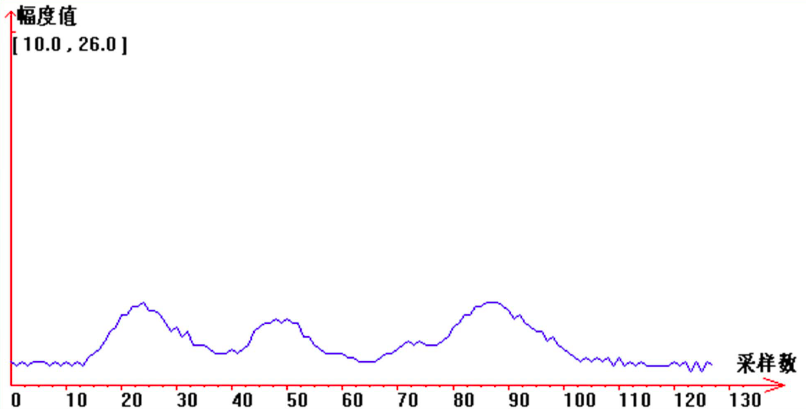
\includegraphics[width=0.7\linewidth]{figure/Chapter4/回波多值性}
			\caption{回波多值性}
			\label{fig:回波多值性}
		\end{figure}
	\item \textit{动态重合系数$ Q $}:激光脚点光斑与接收脚印
		\footnote{由于遥感平台的移动的关系,在反射光束到达接收装置的时候,已经不是原来的激光脚点的位置、大小和形状了,形成接收脚印。由于平台的移动,接收脚印与激光脚点光斑通常只有部分重合。}
		重合部分的面积与激光光斑的面积之比。
		
		\textbf{影响因素}:\begin{itemize*}
			\item 激光波束发散角
			\item 接收瞬时视场角
			\item 传感器平台高度
			\item 扫描镜速度
			\item 波束倾角
		\end{itemize*}
\end{enumerate} % 激光脚点光斑特性

\kaiparagraph{扫描带宽SW}一般来说,激光束扫描角即激光扫描视场角是一个已知量, 在确定飞行高度的情况下,可以计算出扫描带宽:
\begin{equation}
\symrm{SW} = 2H \tan \dfrac{\theta}{2}
\end{equation}
\begin{itemize}
	\item 对于椭圆扫描工作方式仍适用,因为扫描角的量度以天底点方向为准。
	\item 对于Z形扫描,实际扫描宽度长一些。
\end{itemize}

\kaiparagraph{扫描行的点数$ N $}在扫描视场角的范围内可以发射多少束激光,即一扫描行内扫描点的数量。该参数关系到扫描量测点的密度。

根据脉冲重复频率\footnote{每秒钟发射激光脉冲的次数}$ F $和扫描频率\footnote{每秒钟扫描行数}$ f_{sc} $,可计算每一扫描行的点数:
\begin{equation}
N = \dfrac{F}{f_{sc}}
\end{equation}

\textbf{注意}:可见,$ N $与飞行高度和扫描带宽无关。扫描点数计算与飞行高度、扫描带宽无关!
由于不同的区域所需的量测密度不同,当激光扫描仪的扫描频率和脉冲重复频率固定时,即一行扫描点的个数固定;若此时针对具体区域制订飞行计划,要求点的密度要大一些,就要考虑适当降低飞行高度。

\kaiparagraph{激光脚点间距(Point Space)}如图\ref{fig:激光脚点间距}所示,分为航向脚点间距和旁向脚点间距。
\begin{figure}[htbp]
	\centering
	\includegraphics[width=0.7\linewidth]{figure/Chapter4/激光脚点间距}
	\caption{激光脚点间距}
	\label{fig:激光脚点间距}
\end{figure}

\begin{enumerate}
	\item \textit{航向脚点间距$ \diff x_{\text{along}} $}:沿飞行方向扫描点之间的距离称为航向点距。
		\begin{itemize}
			\item \textbf{一般扫描方式}:
				根据飞机飞行速度$ v $,计算得到点距
				\begin{equation}
				\diff x_{\text{along}} = \dfrac{v}{f_{sc}}
				\end{equation}
				式中,$ v $为飞行速度,$ f_{sc} $为扫描频率。可见,航向激光脚点间距也与飞行高度无关,只与飞行速度和扫描频率有关。
			\item \textbf{椭圆扫描方式}:飞行方向上点距较大。
			\item \textbf{Z形扫描方式}:由于有两种定义扫描行的方式,计算飞行方向点距也有两种方式。如图\ref{fig:Z形扫描的激光脚点间距}所示。
				\begin{figure}[htbp]
					\centering
					\includegraphics[width=0.7\linewidth]{figure/Chapter4/Z形扫描的激光脚点间距}
					\caption{Z形扫描的激光脚点间距}
					\label{fig:Z形扫描的激光脚点间距}
				\end{figure}
		\end{itemize} % 航向脚点间距
	\item \textit{旁向脚点间距$ \diff x_{\text{across}} $}:旁向激光脚点间距指一条扫描线上相邻激光脚点的间距,旁向激光脚点间距与扫描带宽SW和每条扫描点上的激光脚点数$ N $相关。
		\begin{itemize}
			\item \textbf{一般扫描方式}:
				\begin{equation}
				\diff x_{\text{across}} = \dfrac{\symrm{SW}}{N}
				\end{equation}
			\item \textbf{光纤扫描}:
				\begin{equation}
				\diff x_{\text{across}} = h \dfrac{\theta}{N-1}
				\end{equation}
			\item \textbf{椭圆扫描}:在接近圆形扫描的情况下,扫描方向点距可按下式作近似估计:
				\begin{equation}
				\diff x_{\text{across}} = \pi \dfrac{\symrm{SW}}{N}
				\end{equation}
				椭圆扫描是由旋转棱镜实现的,根据其镜面和转轴垂面之间的夹角SN,可以较精确地计算扫描方向点距:
				\begin{equation}
				\diff x_{\text{across}} = \dfrac{4.4429 h}{N} \sqrt{\tan^2 \left(2\symrm{SN}\right) + \tan^2 \left(1.41\symrm{SN}\right)}
				\end{equation}
		\end{itemize} % 旁向脚点间距
\end{enumerate} % 激光脚点间距

\kaiparagraph{最少航带数}对于需要进行激光量测的区域,在执行量测任务之前,应对飞行航带数进行估计,若其宽度为$ W $ km ,航带之间扫描重叠度为$ q $。所需航带数为
\begin{equation}
n = \min n_i
\end{equation}
满足
\begin{equation}
(n_i - 1) \geqslant \dfrac{W - \symrm{SW}}{\symrm{SW}(1-q)}
\end{equation}
即
\begin{equation}
n = \symrm{int} \left( \dfrac{W - \symrm{SW}}{\symrm{SW}(1-q)} + 1\right) 
\end{equation}

\textbf{意义}:扫描带宽是一个重要参量,要计算扫描带宽,又与航高有关,
在实际制定飞行计划时,航高的确定须根据区域内的最低点,而航带重叠度的计算则要依据区域内最高点,以避免在扫描带宽很窄的情况下产生遗漏。

\kaiparagraph{实际量测面积}在估算出所需航带数的基础上,可以对激光扫描量测的实际覆盖区域面积进行计算。如果飞机速度为$ v $,待量测区域长度为$ L $,那么,实际量测面积为
\begin{align}
A & = \symrm{SW} v T_S [(n - 1)(1 - q) + 1]
  & = \symrm{SW} L [(n - 1)(1 - q) + 1]
\end{align}

\kaiparagraph{量测点密度}计算出实际量测面积后,实际量测点密度按下式计算:
\begin{equation}
d = \dfrac{FnT_S}{A}
\end{equation}

\kaiparagraph{量测点数据量}实际量测点数据量涉及到数据存储空间的问题,如果需要在飞机上实时计算出地面每一被量测点的三维坐标,并记录下每一个点的反射强度,
每点序号、坐标$ (X,Y,Z) $和时间按4字节记录,强度按一个字节记录,每点需要21个字节,数据总量为
\begin{equation}
C = FT_f \times 21 \text{bytes}
\end{equation}
式中,$ T_f $是激光扫描量测所需的全部时间。

\kaiparagraph{发射及接收激光束间隔内的飞行距离}在激光器发射脉冲到接收地面发射的脉冲有一个时间间隔,在此间隔内一个平台移动了一段距离
\begin{equation}
d = v \times \diff t = \dfrac{2vR}{c}
\end{equation}
一般而言,在以飞机为平台时,这段距离很短。这影响到动态重合系数的大小。

\kaiparagraph{过采样和欠采样}沿扫描方向的估计式为
\begin{equation}
Q_{\text{across}} = \dfrac{2a_L}{\diff x_{\text{across}}}
\end{equation}
如果$ Q_{\text{across}} > 1$,就是过采样,反之就是欠采样。

\section{常用商业LiDAR系统}
\paragraph{Leica公司LiDAR设备}
\paragraph{Optech公司LiDAR设备}
\paragraph{Riegl公司LiDAR设备}
% !TeX spellcheck = <none>
% !TeX encoding = UTF-8
% !TeX root = main.tex

\chapter{LiDAR工程数据获取}%% Chapter05 LiDAR工程数据获取

\paragraph{LiDAR工程步骤}如图\ref{fig:LiDAR工程步骤}所示。
\begin{figure}[h]
	\centering
	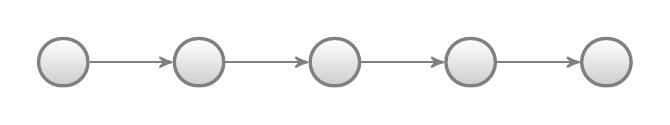
\begin{tikzpicture}[
		terminal/.style = {
			rectangle,minimum size=6mm,rounded corners=3mm,
			very thick,draw=black!50,
			top color=white,bottom color=black!20,
			font=\bfseries
		},
		>=stealth',thick,black!50,text=black,
		graphs/every graph/.style={edges=rounded corners}]
		\matrix[row sep=1mm,column sep=3em] {
			\node    [terminal] (start)		{项目启动}; &
			\node    [terminal]	(get)		{数据获取}; &
			\node    [terminal]	(process)	{数据处理}; &
			\node    [terminal]	(assest)	{精度评定}; &
			\node    [terminal]	(handin)	{提交成果}; \\
		};
		\graph[use existing nodes]{
			start -> get -> process -> assest -> handin;
		};
	\end{tikzpicture}
	\caption{LiDAR工程步骤}
	\label{fig:LiDAR工程步骤}
\end{figure}

\paragraph{LiDAR数据获取综述}
既繁琐又细致的工作,牵扯到许许多多的因
素,需要很多单位和人员的支持和配合。
包含了从飞行准备到航线设计,从飞行操作到
数据整理,从设备运输到存储维护等方方面面
与航测外业相关的作业环节。

\paragraph{三个阶段八个方面}如图\ref{fig:LiDAR数据获取的三个阶段八个方面}所示。
\begin{figure}[htbp]
	\centering
	\includegraphics[width=0.7\linewidth]{figure/Chapter5/LiDAR数据获取的三个阶段八个方面}
	\caption{LiDAR数据获取的三个阶段八个方面}
	\label{fig:LiDAR数据获取的三个阶段八个方面}
\end{figure}

\section{LiDAR数据获取流程}
\subsection{计划准备阶段}

\paragraph{飞行准备}
\begin{enumerate}
	\item \textbf{掌握测区情况}。首先应该熟悉实地测区的地形特点和地貌特征。根据不同的地形条件选择和设计不同的飞行航线。
	\item \textbf{选择LiDAR型号}。国内主要有ALS、ALTM、LiteMapper、 TOPOSYS等产品,每个产品由于性能和参数不同,因此选择不同的设备对于航摄设计来说也是不同的。
	\item \textbf{选择飞行平台}。不同的飞机性能会对雷达系统的参数设置有不同程度的影响。主要有两个方面,一是飞行速度,二是飞行高度。
		\begin{itemize}
			\item 飞行速度主要影响雷达的扫描频率的设置。
			\item 行高度主要影响脉冲频率的设置,进而影响点密度和精度。
		\end{itemize}
	\item \textbf{申请航飞权、协调航空飞行}。流程如图\ref{fig:申请航飞权与协调航空飞行}所示。
		\begin{itemize}
			\item 飞行任务审批。
			\item 机场协调。
			\item 飞行协调。
		\end{itemize}
		\begin{figure}[htbp]
			\centering
			\includegraphics[width=0.7\linewidth]{figure/Chapter5/申请航飞权与协调航空飞行}
			\caption{申请航飞权与协调航空飞行}
			\label{fig:申请航飞权与协调航空飞行}
		\end{figure}
	\item \textbf{制定项目任务书}。在承接航飞任务时,用户单位一般会提交 “项目任务书” ,一般由甲方提出要求,双方技术人员共同拟定。
		\begin{itemize}
			\item 飞行高度
			\item 飞机型号
			\item 航摄分区
			\item 成果坐标系
			\item 野外控制点量测
		\end{itemize}
	\item \textbf{评估飞行效率}。根据测区远近、飞行高度、空域申请情况来编排航飞航线顺序。
\end{enumerate}

\paragraph{航线设计}
\begin{enumerate}
	\item \textbf{步骤}:
		\begin{itemize}
			\item 建立航带设计工程
			\item 设置平面坐标系和高程坐标系
			\item 加载DTM数据
			\item 导入设计线位
			\item 航带设计
			\item 重复以上步骤,完成所有航段的航线设计
		\end{itemize}
		航线设计流程如图\ref{fig:航线设计流程}所示。
		\begin{figure}[htbp]
			\centering
			\includegraphics[width=0.7\linewidth]{figure/Chapter5/航线设计流程}
			\caption{航线设计流程}
			\label{fig:航线设计流程}
		\end{figure}
	\item \textbf{单脉冲和多脉冲}:同等点间距的设计要求下,多脉冲的航飞效率大约为单脉冲的3倍!多脉冲的优势随着地形起伏变化的上升而越加明显。
	\item \textbf{配备数码相机的航线设计}:注意
		\begin{itemize}
			\item 重叠度匹配
			\item 数码相机航向重叠度设置和摄影基线检查
		\end{itemize}
	\item \textbf{最终航线检查与地面模拟飞行}:为了确保飞行计划的正确性。检查方法主要有三种:
		\begin{itemize}
			\item 将飞行计划导出为KML格式,加载到Google Earth当中进行浏览。
			\item 将飞行计划导出到FCMS飞行管理控制软件中进行检查。
			\item 地面模拟飞行。
		\end{itemize}
	\item \textbf{提交航飞设计数据}:完成航线设计之后,需要提交以下材料:
		\begin{itemize}
			\item 飞行记录表
			\item 领航数据表
			\item 飞行文件
			\item 飞行示意图文件
			\item KML文件
		\end{itemize}
\end{enumerate}

\paragraph{检校场的布设、量测}
\begin{enumerate}
	\item \textbf{必要性}:LiDAR设备属于精密仪器,数据采集时要求部件之间有严格的相对位置关系。
		但实际工作中,系统安装时不能完全保证它们相互平行,这些偏差会在设备运输中、设备安装时或者随着时间改变。
	\item \textbf{激光检校场选择及航线设计}:IMU和激光扫描仪的坐标系并不严格平行引起的误差;每次航飞过程中,roll、pitch、heading等会发生变化。
		\begin{itemize}
			\item \textbf{激光检校场布设方案}
				\begin{itemize}
					\item \textit{校准控制场}:校准LiDAR的相对和绝对高程。
					\item \textit{校准建筑物}:校准侧滚和俯仰姿态。
					\item 尽量远离水面(如湖、江)等低反射率的地区。
				\end{itemize}
			\item \textbf{激光检校控制点布设方案}
				\begin{itemize}
					\item 直线控制点:直线大路,2km,每隔5m一个, 高程精度<5cm;
					\item 零散控制点:中心区域均匀10-15点,高程精度 <2cm;
					\item 所有控制点都布设在路面上,且地物材料均匀。
					\item 控制点数据的坐标系为WGS84。
				\end{itemize}
			\item \textbf{激光航线设计方案}:如图\ref{fig:激光检校场布设案例}所示。
				\begin{itemize}
					\item 高航高:通过尖顶房屋正上方过房屋中点,垂直道路及房屋的顶角方向往返飞行各一次(EF、FE);平行于该方向飞行一次(CD);沿道路方向同向飞行一次(AB)。
					\item 低航高:十字飞行(EF,BA)。
				\end{itemize}
				\begin{figure}[htbp]
					\centering
					\includegraphics[width=0.4\linewidth]{figure/Chapter5/激光检校场布设案例}
					\caption{激光检校场布设案例}
					\label{fig:激光检校场布设案例}
				\end{figure}
		\end{itemize}
	\item \textbf{相机检校场选择及航线设计}:相机在安装过程中也会存在和IMU的视准轴不严格一致的情况,这就需要在飞行前或飞行后进行视准轴检校 。
		\begin{itemize}
			\item \textbf{相机检校场布设方案}:从不同方向航线的数据中获取尽可能多的同名地物点,且每一个同名地物点所涉及的航片数量尽可能的多,通过对大量同名点的平差计算,求出相机视准轴与IMU之间的偏差。
				检校场可选择在地物比较丰富的城市地区,覆盖范围一般为6.0 km×4.5 km。城市区域可供选择的特征点比较多,适于后续进行空三计算并寻找足够的连接点,得到较好的检校结果。
			\item \textbf{相机航线设计方案}:相机的焦距不同,检校飞行的航高也不同,一般飞1个高度,采用“十”字对飞,四条航线。如图\ref{fig:相机航线设计方案}所示。
				\begin{figure}[htbp]
					\centering
					\includegraphics[width=0.7\linewidth]{figure/Chapter5/相机航线设计方案}
					\caption{相机航线设计方案}
					\label{fig:相机航线设计方案}
				\end{figure}
			\item \textbf{相机检校控制点布设方案}:
				\begin{itemize}
					\item 测区范围内均匀布设20个控制点,在重叠中心区布设5$ \sim $10个控制点,在航线四个边缘区域总共布设5$ \sim $10个控制点,精度<5 cm。
					\item 控制点选取地物特征点上。
					\item 控制点数据的坐标系为WGS84。
				\end{itemize}
		\end{itemize}
\end{enumerate}

\paragraph{设备安装与测试}
\begin{enumerate}
	\item 开箱验货与货物清点。
	\item 设备安装步骤
		\begin{itemize}
			\item 飞机改造(GPS天线、底舱过渡板、底舱开孔直径与底舱厚度)。
			\item GPS偏心分量测量。如图所示。
				\begin{figure}[htbp]
					\centering
					\includegraphics[width=0.7\linewidth]{figure/Chapter5/GPS偏心分量测量}
					\caption{GPS偏心分量测量}
					\label{fig:GPS偏心分量测量}
				\end{figure}
			\item 设备地面通电测试、记录。
			\item 温度处理。
			\item 数据质量检查与设备状态评估。
		\end{itemize}
\end{enumerate}

\subsection{航飞实施阶段}

\paragraph{基站架设与地面配合}地面配合分为
\textit{检校场地面配合}\footnote{检校场地面配合是针对检校场开展工作, 包括现场确认、检校场标识布设与测量、基站布设与配合观测、控制点测量等方面的工作。}
和\textit{测区地面配合}\footnote{测区地面配合主要包括基站选择与配合观测、野外检查点观测等。}。

\begin{enumerate}
	\item \textbf{检校场基站架设和地面配合}
		\begin{itemize}
			\item 现场勘察
			\item 检校场标识布设
			\item 检校场基站布设
			\item 同步观测
			\item 平面检查点测量
			\item 高程控制点测量
		\end{itemize}
	\item \textbf{测区基站架设和地面配合}
		\begin{itemize}
			\item 一般地区基站布设
			\item 困难地区基站布设
			\item 检查点测量
		\end{itemize}
	\item 基站工作注意事项
\end{enumerate}

\paragraph{飞行操作与数据采集}
\begin{enumerate}
	\item \textbf{GPS星历预测}:LiDAR在空中工作时,需要实时锁定卫星接收GPS信号,并且卫星星座分布的几何强度直接决定着卫星测距的误差。
		在实际飞行之前,需要对当天点位的三维精度因子(PDOP)进行预测。有些商用软件(GrafNav)可以通过网络下载卫星星历预报数据来计算出某天某一时刻的PDOP值以及 卫星数目。
	\item \textbf{地面通电测试与准备工作}
	\item \textbf{飞行质量要求}如图\ref{fig:飞行质量要求}所示。
		\begin{itemize}
			\item 8字飞行
			\item 地面静态观测
			\item 盘旋转弯坡度要求
			\item 飞行姿态要求
			\item 飞行速度要求
		\end{itemize}
		\begin{figure}[htbp]
			 \centering
			 \includegraphics[width=0.7\linewidth]{figure/Chapter5/飞行质量要求}
			 \caption{飞行质量要求}
			 \label{fig:飞行质量要求}
		\end{figure}
	\item \textbf{飞行作业和设备空中操作}:空中操作是固定而且单一的,高级的激光
		雷达设备在使用操作上往往十分简单,用
		户只需进行触动几个按钮就可以完成整个
		航飞任务,其他所有工作都让计算机来监
		视完成。
	\item 激光扫描测量
	\item GPS/IMU定位定向测量
	\item 数码相机拍摄
	\item 空中异常情况及处理
\end{enumerate}

\subsection{数据整理阶段}
\paragraph{数据检查与质量控制}
\begin{enumerate}
	\item \textbf{数据整理归档}
	\item \textbf{日志文件}
	\item \textbf{数据质量检查}
		\begin{itemize}
			\item GPS/IMU数据解压
			\item 导航文件精度指标
			\item 激光数据检查
			\item 影像数据检查
		\end{itemize}
	\item \textbf{补飞和重飞}
\end{enumerate}

\paragraph{数据预处理}
\begin{enumerate}
	\item \textbf{目的}:
		\begin{itemize}
			\item 三维坐标解算
			\item 坐标转换
			\item 文件生成
		\end{itemize}
	\item \textbf{数据预处理流程}:如图\ref{fig:数据预处理流程}所示。
		\begin{figure}[htbp]
			\centering
			\includegraphics[width=0.5\linewidth]{figure/Chapter5/数据预处理流程}
			\caption{数据预处理流程}
			\label{fig:数据预处理流程}
		\end{figure}
	\item \textbf{SBET (Smoothed Best Estimated Trajectory)航迹文件处理}:GPS差分处理(GPS数据+基站数据)。每条航带一个航迹文件,处理软件 POSProc。
	\item \textbf{位置内插}。如图所示。
		\begin{figure}[htbp]
			\centering
			\includegraphics[width=0.5\linewidth]{figure/Chapter5/位置内插}
			\caption{位置内插}
			\label{fig:位置内插}
		\end{figure}
	\item \textbf{“*.LAS” 文件——ALS Post Processor}
		\begin{itemize}
			\item 解算每个目标点的三维坐标;
			\item 每条航带生成一个二进制格式的LAS文件;
			\item 存储格式为lat/lon/el/intensity data 或者 northing/easting/el/intensity in user-selected projection;
			\item 记录顺序:shot-by shot, return by return。
		\end{itemize}
	\item \textbf{生成 “quick-look edge-of-coverage” 高程图 ( *.TIF)}
\end{enumerate}

\paragraph{调整航带间点云不一致}如图\ref{fig:调整航带间点云不一致}所示。
\begin{figure}[htbp]
	\centering
	\subfloat[原始点云]{\includegraphics[height=2.5cm]{figure/Chapter5/原始点云}}
	\subfloat[调整前点云]{\includegraphics[height=2.5cm]{figure/Chapter5/调整前点云}}
	\subfloat[调整后点云]{\includegraphics[height=2.5cm]{figure/Chapter5/调整后点云}}
	\caption{调整航带间点云不一致}
	\label{fig:调整航带间点云不一致}
\end{figure}

\paragraph{坐标变换}由WGS84坐标系大地坐标变换为地方局部坐标系坐标。
\begin{itemize}
	\item \textbf{投影变换}
		\begin{itemize}
			\item Gauss投影
			\item UTM投影
			\item Mercator投影
			\item Lambert投影
			\item Albers投影
		\end{itemize}
	\item \textbf{椭球变换}
		\begin{itemize}
			\item \textit{七参数法}(包括布尔莎模型、一步法模型、海尔曼特等),即$ X $平移,$ Y $平 移,$ Z $平移,$ X $旋转,$ Y $旋转,$ Z $旋转,尺度变化$ K $。
			\item \textit{三参数}(莫洛登斯基模型),即$ X $平移,$ Y $平移,$ Z $平移,而将$ X $旋转,$ Y $旋转,$ Z $旋转,尺度变化$ K $视为0,所以三参数只是七参数的一种特例。
		\end{itemize}
\end{itemize}

\paragraph{文件生成}
\begin{enumerate}
	\item \textbf{LAS格式}:美国摄影测量与遥感协会提出Lidar Data Exchange Format Standard (LDEFS) 1.0标准。
		\begin{itemize}
			\item \textbf{公共数据块(Public Header Block)}:公共数据块的大小是227 bytes,记录了关于该文件的一些基本信息,
				如:文件标识、飞行时间、回波个数、坐标范围等等,详细描述了关于las数据采集的信息。
			\item \textbf{变长数据记录(Variable length Records)}。
			\item \textbf{点数据块(Point data)}。
			\item \textbf{变长的波形记录}(1.3格式)。
		\end{itemize}
	\item \textbf{ASC栅格格式}:一些公司采用了栅格文件格式作为Lidar的数据格式。例如,采用ArcInfo Grid格式的数据作为通用格式。
		\begin{itemize}
			\item \textbf{头部信息}:
				\begin{itemize}
					\item ncols行数
					\item nrows列数
					\item xllcenter中心点x坐标
					\item yllcenter中心点y坐标
					\item cellsize采样间距
					\item NODATA\_value -9999.000000(无效数据)
				\end{itemize}
			\item \textbf{数据信息}:记录具体的信息数据。
		\end{itemize}
	\item \textbf{自定义TXT格式}:这种格式直接以文本的方式记录LiDAR数据,每 一行记录一束激光的回波数据,以不同的列记录不同属性的数据,一般会在数据中加以说明。
\end{enumerate}

\paragraph{点云数据特点}LiDAR激光脚点的分布是按照时间序列进行采样和存储的,其在地面上的分布不是规则的,其空间分布呈现为离散的数据”点云”(Points Cloud)。如图\ref{fig:点云数据特点}所示。
\begin{figure}[htbp]
	\centering
	\subfloat[激光脚点]{\includegraphics[height=4cm]{figure/Chapter5/点云数据特点_脚点}} \quad
	\subfloat[点云]{\includegraphics[height=4cm]{figure/Chapter5/点云数据特点_点云}}
	\caption{点云数据特点}
	\label{fig:点云数据特点}
\end{figure}

\section{LiDAR技术与同类技术对比}

% !TeX spellcheck = <none>
% !TeX encoding = UTF-8
% !TeX root = main.tex

\chapter{LiDAR数据处理} % Chapter LiDAR数据处理

\section{点云滤波} 
\subsection{点云滤波概述}

\paragraph{点云滤波的目的}
\begin{itemize}
	\item LiDAR点云包括:地面点、 房屋点、树木、交通工具……。通过点云滤波来提取地面点,剔除非地面点。
	\item 基于LiDAR点云生成DEM:从点云中识别出地面点,并剔除建筑物、树木等非地面点,接着利用地面点生成DEM。
\end{itemize}

\paragraph{基于LiDAR数据生成DEM的工作}
\begin{itemize}
	\item 点云滤波
	\item DEM内插
	\item DEM精度分析
\end{itemize}

\paragraph{点云(距离数据)空间分布特征}
\begin{itemize}
	\item 地形平坦区域,由于激光脉冲的发射频率一般是固定的,激光点云在空间上成规则分布;
	\item 植被覆盖区域,点云之间的规则间隔被打破,由于脉冲可以穿透植被形成多次回波,空间分布成团聚等不规则形状;
	\item 水、云、雨或烟雾等能吸收近红外波段的激光脉冲,造成局部区域的点云缺失;
	\item 玻璃、光亮金属或建筑物边缘等表面的强反射,以及脉冲的折射、多路效应等,会引起点云的$ x $、$ y $或$ z $值异常,产生噪点。
\end{itemize}
一般情况下:
\begin{itemize}
	\item 建筑物和高大植被点云都具有较大的$ z $值(在城区,最大$ z $值的点云一般都是建筑物);
	\item 裸露地表点云的$ z $值最小;
	\item \textit{地面突出物}(如围墙、立交桥、花坛等)和灌丛点云的$ z $值介于两者之间;
\end{itemize}
这些地物在垂直方向上形成层次分布,而在
相邻地物之间,由于地面与地物的高度差异明显,
往往表现出高程突变现象,这就为地面点的识别
提供了依据。

\paragraph{基于高程突变的的滤波方法基本前提}
\begin{itemize}
	\item DSM中非地面点高于地面点(DEM)
	\item 地面点高程变化不会太大
\end{itemize}

\paragraph{自动滤波算法的难点}
\begin{enumerate}
	\item 局外点的影响,如图\ref{fig:局外点的影响}所示。
		\begin{figure}[htbp]
			\centering
			\quad\quad
			\subfloat[高的局外点]{\includegraphics[height=3.5cm]{figure/Chapter6/高的局外点}} \hfill
			\subfloat[低的局外点]{\includegraphics[height=3.5cm]{figure/Chapter6/低的局外点}} \hfill
			\subfloat[低的局外点导致侵蚀]{\includegraphics[height=3.5cm]{figure/Chapter6/低的局外点导致侵蚀}} \quad\quad
			\caption{局外点的影响}
			\label{fig:局外点的影响}
		\end{figure}
	\item 对象的复杂性、附着对象、点云分布不均匀、有断裂。
\end{enumerate}

\paragraph{滤波精度分析方法}
\begin{enumerate}
	\item \textit{第一类错误率}(Type I):将地面点分为地物点。
	\item \textit{第二类错误率}(Type II):将地物点分为地面点。
	\item \textit{总错误率}
\end{enumerate}

\paragraph{LiDAR点云滤波研究现状}如表\ref{tab:LiDAR点云滤波研究现状}所示。
\begin{table}[htbp]
	\centering
	\caption{LiDAR点云滤波研究现状}
	\label{tab:LiDAR点云滤波研究现状}
	\begin{tabular}{|l|l|}
		\hline
		假设条件         & 存在问题                        \\ \hline
		非地面点均高于地面点   & 由于粗差、多路径效应等,造成最低点并非理想地面点数据。 \\ \hline
		激光点可穿透树林到达地面 & 植被非常密集的地区,激光点难以穿过树林。        \\ \hline
		地形坡度不会过大     & 在平坦地区此假设有效,对坡度大的山区,并不总是满足   \\ \hline
	\end{tabular}
\end{table}

\paragraph{滤波算法研究趋势}
\begin{itemize}
	\item 高精度
	\item 全自动
	\item 高性能运算
	\item 融合辅助数据源的滤波优化算法
\end{itemize}

\subsection{典型滤波方法}

\kaiparagraph{一维双向扫描标记法}
\begin{enumerate}
	\item \textbf{算法思想}
		\begin{itemize}
			\item 认为非地面点与地面点构成的坡度大于地面点之间构成的坡度;
			\item 认为地面点的高程,低于邻域非地面点的高程。
		\end{itemize}
	\item \textbf{地面店判别条件}:
		\begin{equation}
		\forall P_i : \left\lbrace \begin{array}{ll}
		S_v > S_T ∧ Z_i > Z_T, & \text{地面点} \\
		\text{else},			& \text{非地面点}
		\end{array} \right.
		\end{equation}
	\item \textbf{算法步骤}
		\begin{enumerate}
			\item \textbf{基于高程和坡度条件扫描标记出初始地面点}:假设起始点为房屋点,根据坡度与高程阈值按从右到左、从左到右进行识别标记
				\begin{equation}
				S_i = \arctan \left[ \dfrac{Z_i - Z_{i-1}}{\sqrt{\left(X_i - X_{i-1}\right)^2 + \left(Y_i - Y_{i-1}\right)^2}} \right],\quad S_i \in \left[-\dfrac{\cpi}{2}, \dfrac{\cpi}{2}\right]
				\end{equation}
			\item \textbf{基于线性衰退法进一步去除非地面点}:认为局部区域地面点构成坡度一致,利用线性衰减法进一步去除非地面点
				\begin{equation}
				Z = a_0 + a_1D, \quad D < D_T
				\end{equation}
		\end{enumerate}
	\item \textbf{实例}:如图\ref{fig:一维双向扫描标记法算法步骤}所示。
		\begin{figure}[htbp]
			\centering
			\subfloat[原始点云]{\includegraphics[height=3cm]{figure/Chapter6/一维双向扫描标记法-原始点云}} \quad
			\subfloat[从右往左]{\includegraphics[height=3cm]{figure/Chapter6/一维双向扫描标记法-从右往左}} \quad
			\subfloat[从左往右]{\includegraphics[height=3cm]{figure/Chapter6/一维双向扫描标记法-从左往右}} \\
			\subfloat[取交集]{\includegraphics[height=3cm]{figure/Chapter6/一维双向扫描标记法-取交集}} \quad\quad\quad
			\subfloat[线性衰减]{\includegraphics[height=3cm]{figure/Chapter6/一维双向扫描标记法-线性衰减}}
			\caption{一维双向扫描标记法算法步骤}
			\label{fig:一维双向扫描标记法算法步骤}
		\end{figure}
\end{enumerate}

\kaiparagraph{TopScan算法}
\begin{enumerate}
	\item \textbf{步骤过程}:
		\begin{itemize}
			\item 采用比较大的移动窗,在窗中搜索最低点,由每次移动窗中找出的最低点的全体,形成了一个初步的地面模型。
			\item 将所有的点与此模型比较,在每一点上形成高差,凡高差超过某个阈值,被认为是非地面点,将这些点滤除。
			\item 减小窗口,重复第一、二步工作,搜索最低点,形成地面模型,改变阈值,滤除与地面模型高差大的点,重复数次以后得到比较精确的地面点高程数据集合 。
		\end{itemize}
	\item \textbf{窗口和滤波阈值大小的选取}:
		\begin{itemize}
			\item 窗口小,就可能将一些大房屋顶点保留下来;窗口太大 则会将地表面“平滑”,使微小的地形变化部分被滤除。
			\item 阈值太大,会将一些植被点作为地面点保留下来;阈值太小,可能将真实的较小的地形突变点去掉;
			\item 窗口和阈值大小与实际地形地貌密切相关。不同的地域, 如平原、丘陵、山地,应该有不同的参量。
		\end{itemize}
\end{enumerate}

\kaiparagraph{基于多分辨率方向预测的点云滤波算法}
\begin{enumerate}
	\item \textit{线性预测法}:若相邻两点距离比较近,而且二者的高程相差较小,则认为这两点为同一类型点的可能性比较大;
		否则较高点为地物点的可能性比较大。
		当然随着两点之间的距离的加大,较高点为地物点的可能性也随之减小。
			
		假设集合$ S $为原始LiDAR点云,则地面点集合$ S_T $可以表示为
		\begin{equation}
		S_T = \left\lbrace p_i \in S \left| ∀p_j \in S : h_{p_i} - h_{p_j} \leqslant Δh_{\max} \left( d(p_i,p_j) \right) \right. \right\rbrace
		\end{equation}
	\item \textit{方向预测法}:在某一距离范围内,若当前点与所有方向预测值的差值均大于该距离条件下的最大高差限差,则该点为地物点,否则为地面点。
	
		对于原始LIDAR点云属于集合$ S $,方向数据集$ S_{\text{dir}} \in S $,则地物点数据集$ S_O $可以表示为
		\begin{equation}
		S_T = \left\lbrace p_i \in S \left| ∀p_j,p_k \in S_{\text{dir}} : h_{p_i} - h(p_j,p_k) > Δh_{\max} \left( d(p_j,p_k) \right) \right. \right\rbrace
		\end{equation}
		则地面点数据集$ S_T $可以表示为
		\begin{equation}
		S_T = S - S_O
		\end{equation}
	\item \textit{多分辨率方向预测处理}:采用类似影像金字塔的方式,构建不同分辨率的数据集,以分辨率由低到高的次序依次进行平滑处理。邻域方向如图\ref{fig:邻域方向}所示。
		\begin{figure}[htbp]
			\centering
			\includegraphics[scale=0.5]{figure/Chapter6/邻域方向}
			\caption{邻域方向}
			\label{fig:邻域方向}
		\end{figure}
\end{enumerate}

\kaiparagraph{移动曲面滤波方法}
\begin{enumerate}
	\item \textbf{算法原理}:激光点云的空间关系反映了地形表面的空间变化,任何一个复杂的空间曲面,其局部面元可利用一个简单的二次曲面拟合
		\begin{equation}
		Z_i = f(X_i,Y_i) = a_0 + a_1 X_i + a_2 Y_i + a_3 X_I^2 + a_4 X_i Y_i + a_5 Y_i^2
		\end{equation}
		当局部面元小到一定程度,甚至可以将该局部面元近似表达成一个平面
		\begin{equation}
		Z_i = f(X_i,Y_i) = a_0 + a_1 X_i + a_2 Y_i
		\end{equation}
	\item \textbf{算法步骤}
		\begin{itemize}
			\item 选择初始地面种子点。选择局部最低的三个点作为种子点(图\ref{fig:移动曲面滤波算法1})。
			\item 进行初始平面拟合(图\ref{fig:移动曲面滤波算法2})。
			\item 基于平面拟合方程判别邻近激光点。当拟合点数达6个时,改用二次曲面方程进行地形拟合(图\ref{fig:移动曲面滤波算法3})。
			\item 基于二次曲面方程进行地面点的迭代判 别,并不断更新地形曲面,完成LiDAR点云的滤波(图\ref{fig:移动曲面滤波算法4})。
		\end{itemize}
		\begin{figure}[htbp]
			\centering
			\subfloat[]{\label{fig:移动曲面滤波算法1}\includegraphics[height=2.2cm]{figure/Chapter6/移动曲面滤波算法1}} \hfill
			\subfloat[]{\label{fig:移动曲面滤波算法2}\includegraphics[height=2.2cm]{figure/Chapter6/移动曲面滤波算法2}} \hfill
			\subfloat[]{\label{fig:移动曲面滤波算法3}\includegraphics[height=2.2cm]{figure/Chapter6/移动曲面滤波算法3}} \hfill
			\subfloat[]{\label{fig:移动曲面滤波算法4}\includegraphics[height=2.2cm]{figure/Chapter6/移动曲面滤波算法4}}
			\caption{移动曲面滤波算法}
			\label{fig:移动曲面滤波算法}
		\end{figure}
	\item \textbf{难点}:该算法的难点在于种子点的选择以及滤波阈值的确定。种子点选择不恰当会使得曲面迭代拟合结果陷入极值,无法得到正确结果;同时滤波阈值需要根据地形起伏自适应地变化,否则难以取得较好的效果。
\end{enumerate}

\kaiparagraph{基于TIN加密的点云滤波方法}
\begin{enumerate}
	\item \textbf{原理}:
		\begin{itemize}
			\item 获取一定的地面种子点组成初始的稀疏不规则三角网;
			\item 对各点进行判断,如果该点到三角面的垂直距离及角度小于设定的阈值,将该点加入地面点集合,实现TIN的不断 加密。
			\item 重新计算不规则三角网,然后再对非地面点集合内的点进行判别。
			\item 如此迭代,直到不再增加新的地面点,或者满足给定条件为止。
		\end{itemize}
	\item \textbf{过程}:
		\begin{itemize}
			\item 采用逐级内插
			\item 逐步迭代,由粗到细的内插方法。
			\item 迭代条件:
				\begin{itemize}
					\item 点与三角形的夹角不能大于一定的限度。
					\item 点与所在三角形的距离不能大于一定的限度。
				\end{itemize}
		\end{itemize}
	\item \textbf{种子点选取思路}:建筑物一般不会覆盖较大的区域(譬如: 80m × 80m)。这个范围内的低点一般是地面点。
	\item \textbf{难点}:
		\begin{itemize}
			\item 需要先将低的噪声点去除,否则会造成没有点可以选入的情况。
			\item 对于低矮植被不容易去除。
			\item 对于陡峭的小山坡也会发生错分的情况。
		\end{itemize}
\end{enumerate}

\paragraph{其他滤波算法}
\begin{enumerate}
	\item \textit{基于数学形态学滤波方法}
	\item \textit{基于TIN的改进滤波方法}
	\item \textit{基于区域增长的点云滤波方法}
\end{enumerate}

\subsection{DEM生成}
\paragraph{DEM内插}地面空白填补滤波之后产生了一些空缺点,如房屋顶点滤除后,应补上所在位置的高程。
\begin{enumerate}
	\item \textit{反距离权重法}(inverse distance weighting)
		\begin{equation}
		f(P) = \left\lbrace \begin{array}{ll}
		\dfrac{\displaystyle{\sum_{i=1}^{n} d_i^{-u} Z_i}}{\displaystyle{\sum_{i=1}^{n} d_i^{-u}}} & ∀P_i,d_i \neq 0 \\
		Z_i & ∃P_i,d_i = 0
		\end{array} \right.
		\end{equation}
	\item \textit{多项式插值法}(interpolating polynomials)
	\item \textit{最近点插值法}(Nearest Neighbor)
	\item \textit{克立格插值法}(Kriging)
\end{enumerate}
不同的插值方法对应不同的插值精度以及插值效率,也适用于不同的插值用途。

\paragraph{DEM模型}
\begin{enumerate}
	\item \textit{规则格网模型}:根据生成DEM的要求,如范围、间距等,由邻近地面点的位置(即$ (X,Y) $坐标)内插规则格网点上的高程才能最终产生 DEM。
	\item \textit{不规则三角网模型}(TIN):直接基于离散地面点构建Delaunay三角网。
	\item \textit{混合模型}:规则格网+TIN。在地形变化小的地方采用低分辨率的规则格网,在地形变化大的地方用TIN。
\end{enumerate}

\subsection{精度分析}

\paragraph{叠加对比分析}如图\ref{fig:叠加对比分析}所示,由激光扫描数据生成的等高线(浅色);由摄影测量方法生成的等高线(深色)。
\begin{figure}[htbp]
	\centering
	\includegraphics[width=0.8\linewidth]{figure/Chapter6/叠加对比分析}
	\caption{叠加对比分析}
	\label{fig:叠加对比分析}
\end{figure}

\paragraph{抽样统计分析}选择植被较少或没有植被的平坦地区作为检查区域,与差分GPS测量结果进行比较,得到高程残差统计图。如图\ref{fig:抽样统计分析}所示。
\begin{figure}[htbp]
	\centering
	\includegraphics[width=0.8\linewidth]{figure/Chapter6/抽样统计分析}
	\caption{抽样统计分析}
	\label{fig:抽样统计分析}
\end{figure}

\paragraph{LiDAR的优势}
\begin{itemize}
	\item \textbf{费用成本低}:与摄影测量方法比较,所需费用只是其25\%$ \sim $33\%,节省了山区林地地面实测的费用、内业处 理的费用等。
	\item \textbf{限制条件少}:飞行季节、时间、天气的限制较少。
		\begin{itemize}
			\item 冬季也可以进行,既便有雪也无碍;
			\item 白天黑夜都可以工作;
			\item 在阴天,云下飞行扫描同样有较好的结果。
		\end{itemize}
\end{itemize}

\paragraph{建议}
\begin{itemize}
	\item \textbf{时间}:最好在11月到第二年三月间进行;
	\item \textbf{天气}:最好选择无雪、无雨的日子;
	\item \textbf{参量}:飞行和扫描参量根据各种不同需要,在飞行前要认真讨论确定;扫描点的分布要尽可能有规律;对于10 m格网间距高程精度要求数分米的DEM,平均扫描点距不要超过5m。
	\item \textbf{基站}:用于GPS差分处理,对于提高精度非常重要;
	\item \textbf{检测区域}:要选择平地或斜地,植被复盖尽可能少, 量测点密,量测精度要优于1 dm;
	\item \textbf{检测}:95\%的点的精度优于3 dm的情况下才算合格。
\end{itemize}

\section{强度数据处理}
商用LiDAR系统在获取三维位置坐标信息(距离)数
据的同时都可以记录下各激光脚点反射的回波信号的
强度信息。由于强度信息的本质同传统的光学影像是
一样的,大多数学者倾向于采用传统的数字图像处理
的方法来处理。

\subsection{强度数据特点}
\begin{enumerate}
	\item 噪声大
	\item 未定标
	\item 与距离信息同时获取
	\item 与光学影像相似
\end{enumerate}

\subsection{强度数据校正}LiDAR系统记录的强度值与接收回波信号能力成正比,
因为为了使得强度值真实反映目标的反射特性,必须
去掉距离、瞬时角度以及大气和传感器参数等外部影
响。

依据激光雷达方程
\begin{equation}
P_r = \dfrac{\eta_o \rho T_a^2 A_r}{\pi R^2} \cdot \dfrac{A_i}{A_b}P_t
\end{equation}
式中,$ P_r $是激光雷达接收到的激光功率;$ P_t $是光学系统效率;$ \rho $是目标表面反射率,$ T_a $是单程大气透过率,$ A_r $是光学系统有效接触面积,$ R $是目标与激光雷达的距离;$ A_i $是目标被照面积(截面积);$ A_b $是目标处的光斑面积。
经推导得到
\begin{equation}
P_r = \dfrac{P_t D_r^2 \rho}{4R^2} \cos \theta_i \eta_{\text{sys}} \eta _{\text{atm}}
\end{equation}
式中,$ \theta_i $为瞬时角度,$ \eta_{\text{sys}} $为系统发射因子,$ \eta _{\text{atm}} $为大气影响因子。

可借助接收功率与距离、角度等比例关系进行强度校正!

\subsection{强度图像生成处理}
\begin{enumerate}
	\item \textbf{重采样}:将时间序列的数据转换为规则格网数据阵列,每个像素值代表该点对应的回波强度值。
	\item \textbf{去粗差}
	\item \textbf{去噪}:LiDAR强度信息存在着较严重的噪声,噪声中的主要成份为脉冲噪声(椒盐噪声),其概率密度函数(PDF)一般为指数密度分布和伽马密度分布。这种噪声为乘性噪声,与信号相关,本质上是非线性的,难以去除。
		\begin{itemize}
			\item \textit{中值滤波去噪}:常用的非线性滤波方法。中值滤波对脉冲 干扰及椒盐噪声的抑制效果好,在抑制随机噪声的同时,造成边缘模糊成度小。
			
				\textbf{做法}:对一个滑动窗口内的所有像素灰度值排序,用中值作为窗口中心像素输出值的处理。
			\item {\kaishu 针对城区LiDAR强度数据的去噪}
			\item {\kaishu 基于平坦度的LiDAR强度图像去噪}:适用非城区数据处理。
		\end{itemize}
\end{enumerate}

\subsection{应用案例}

结合LiDAR强度和距离信息实现道路的自动提取。

\section{基于LiDAR数据的建筑物提取}

\paragraph{建筑物提取的方法}
\begin{enumerate}
	\item \textbf{基于光学影像的方式}
		\begin{itemize}
			\item 利用单幅影像阴影分析的方法,或直接通过边缘检测获取建筑物边界的方法。
			\item 利用立体像对进行人工判读(模拟及解析测量的成图方式),提取建筑物的方法;
				或利用数字摄影测量工作站进行半自动或全自动的建筑物提取。
		\end{itemize}
	\item \textbf{基于LiDAR点云的方式}:基于LiDAR点云进行建筑物提取即模型重建。
		\begin{itemize}
			\item 建筑物检测(分割)
			\item 建筑物模型生成(重建)
		\end{itemize}
\end{enumerate}

\paragraph{两种提取方法的不同}基于影像的建筑物提取方法与基于LiDAR的建筑物提取方法的不同之处如表\ref{tab:建筑物两种提取方法的不同}所示。
\LTXtable{\linewidth}{table/建筑物两种提取方法的不同}

\subsection{建筑物检测(分割)}

\kaiparagraph{分割}由激光扫描数据建立房屋模型,首先必须将房屋点从点云数据中识别、提取出来。

\paragraph{一般步骤}
\begin{enumerate}
	\item 检测出建筑物激光脚点数据
	\item 确定各建筑物激光脚点所属的建筑物,即建立多对一的映射关系。
\end{enumerate}

\paragraph{现有分割方法}
\begin{itemize}
	\item 在数据密度足够大,地面起伏不大的情况下,可采取局部极值检测方法,并以极值点为中心进行局部直方图分析,得到合理的阙值,实现房屋点的检测。
	\item 采取滤波方法来辅助建筑物的提取。滤波是为了滤除非地面点,可用于房屋点的提取。
	\item 利用激光扫描回波强度数据,作为分析房屋的辅助数据。如对于近红外激光,植被的反射率很高,可以用来区分房屋和植被,但这种反射率数据质量一般较差。
	\item 利用辅助数据源:
		\begin{itemize}
			\item 利用二维GIS信息,即利用已有的图形数据,辅助建筑物数据的提取。但需要注意实际的屋顶面常常比图形数据所显示的面积要大。
			\item 利用影像光谱信息,现有的LiDAR系统在飞行时,会同时载有多光谱和高光谱扫描仪,其影像数据将大大有利于房屋的提取。
		\end{itemize}
\end{itemize}

\paragraph{涉及的处理方法}:高度直方图分析、形态滤波等方法、房屋最低高度阙值、最小屋顶面积等:

\subsection{建筑物模型的生成(重建)}
\paragraph{任务}提取矢量化的建筑物模型。

\paragraph{现状}虽然LiDAR提供了丰富的建筑屋顶面\footnote{屋顶面虽然仅仅是建筑物模型的一个重要部分,但几乎所有的建筑物模型重建研究都集中于屋顶模型的重建。}的信息,但是,由于建筑物结构复杂,自动化程度较高的建筑物模型重建算法、商用软件并没有出现。

\paragraph{建筑物提取的典型方法}
\begin{itemize}
	\item 基于三角网的房屋模型重建方法
	\item 基于不变矩的建筑物提取方法
	\item 自适应迭代的DSM影像分割方法
	\item 基于边界表达的建筑物模型重建方法
	\item 其他:基于特征线的数据驱动方法、Hough变换以及其扩展变换、模型驱动的方法……
\end{itemize}

\kaiparagraph{基于三角网的房屋模型重建方法}
\begin{enumerate}
	\item 分割建筑物点,并构建三角网
	\item 分析三角面元,确定屋顶平面。
		\begin{itemize}
			\item 对每一个小三角平面都可以根据三个定点的坐标,计算出两个坡度参量$ S_x$、$ S_y $和一个距离参量$ d $,因为每一个平面可由下式描述
				\begin{equation}
				Z = S_x X + S_y Y + d
				\end{equation}
			\item 计算出所有小平面的上述参量,形成一个三维参量聚类空间,参量相同的小平面在同一个屋顶面内。
		\end{itemize}
	\item 提取边界线。将各个屋顶面参量求解出来之后,就可以提取边界线和屋脊线。如果有多条脊线,则最长的脊线代表房屋的主方向。
	\item 进行边界优化和拟合
		\begin{enumerate}
			\item 前提条件:
				\begin{itemize}
					\item 边缘线与代表房屋方向的屋脊线平行或垂直;
					\item 主方向的边缘点应当是高程等值点。
				\end{itemize}
			\item 拟合流程:对分割后数据集中处于边缘上的点进行分析:
				\begin{itemize}
					\item 从其中任意一点出发,找到相邻点之后即初步估计出连线的方向,计算出连线的直线方程。
					\item 按该直线方向与房屋走向的关系进行调整,后续点根据它与该直线的距离是否超过某一阂值,决定它是否为该直线方向的边缘点,当超过阂值就是另一条边缘直线的开始点。
					\item 对于初步的搜索结果通过最小二乘拟合进一步优化,使所有边缘点到边缘线的距离平方和最小。
					\item 拟合结果并非边缘线的真正位置,因为边缘线应当将所有边缘点都围在所形成的多边形内,要尽可能使边缘点处于边界内。
					
					可以利用墙面点信息,对边缘线位置作一点调整,墙面点信息是被分割的屋顶点集以外的点,有助于屋顶边缘线的确定,也有助于计算墙面高度。
				\end{itemize}
		\end{enumerate}
\end{enumerate}

\kaiparagraph{利用不变矩提取房屋模型}
\begin{enumerate}
	\item 对于连续函数,矩的定义
		\begin{equation}
		M_{ij} = \int_{x_1}^{x_2}\int_{y_1}^{y_2} x^i y^j f(x,y) \diff x \diff y
		\end{equation}
		LiDAR数据是离散数据,分割之后,按分割的子集分别计算其矩,并以\textbf{高程值作为权重},则矩的定义
		\begin{equation}
		M_{ij} = \sum_{p=p_i}^{p_n} x_p^i y_p^j H_p
		\end{equation}
		$ H_p $为子集$ {p_1,p_2,\cdots,p_n} $中某点的高程。
		
		\textit{不变矩}是各坐标重心化之后,相应于个子集重心的矩。
			\begin{itemize}
				\item \textit{平移不变矩}
				\item \textit{比例不变矩}
				\item \textit{旋转不变矩}
			\end{itemize}
		
		对于灰度化的数据,$ H_p = 1 $,可以得到二值矩$ m_{ij} $定义如下
		\begin{equation}
		M_{ij} = \sum_{p=p_i}^{p_n} x_p^i y_p^j
		\end{equation}
		注意:房屋的参量必须由归一化矩计算得到,即与除以$ m_{00} $进行归一化处理。
	\item 房屋类型的确定:可以通过比较带高程权重的二阶矩与灰度化二阶矩得到,即
		\begin{equation}
		r_q = \dfrac{M_{20}/M_{02}}{m'_{20}/m'_{02}}
		\end{equation}
		\begin{itemize}
			\item 若$ rq=1 $,则屋顶为平面;
			\item 若$ rq>1 $,则屋顶面与房屋主轴平行;
			\item 若$ rq<1 $,则屋顶面与房屋主轴垂直。
		\end{itemize}
	\item 一般步骤
		\begin{itemize}
			\item 房屋点的分割
			\item 确定房屋特征参数与不变矩函数关系式
			\item 计算不变矩,导出房屋特征参数
			\item 利用房屋点及特征参数,计算房屋特征点坐标,并重建房屋模型。
		\end{itemize}
	\item 不变矩的方法常用于计算具有平面或人字形屋顶的房屋的参数。其他屋顶类型的确定需要计算更高阶的矩。更高阶的矩还可以检测屋顶的不对称性。
	\item 不同屋顶类型的处理方法
		\begin{itemize}
			\item 不对称屋顶:首先利用矩确定标
				准的人字形屋顶类型:然后根据实际点云与标准
				模型之间的差异,将其他点(烟囱、天窗、天线
				等)分割出来:最后进一步利用不变矩来分析,
				提取其参数。
			\item 复杂屋顶:将屋顶分割为多个单元,如基元屋
				顶,然后分别提取这些基元屋顶的参数:
			\item 底面形状非矩形的屋顶:不推荐采用高阶不变矩分析的方法来确定其模型。
		\end{itemize}
\end{enumerate}

\kaiparagraph{自适应迭代的DSM影像分割方法}
\begin{enumerate}
	\item \textbf{处理流程}
		\begin{multicols}{2}
			\begin{enumerate}
				\item 城市DSM数据
				\item 中值滤波平滑
				\item 图像阙值分割
				\item 提取建筑物的边界
				\item 建筑物边界眼踪
				\item 去除不闭合的边界
				\item 多边形逼近建筑物
				\item 边界点的分组和拟合方位角
				\item 确定或给定建筑物主方向
				\item 建筑物各边缘线段规格化
				\item 边缘规格化效果评价
				\item 计算建筑物的高度
				\item 建筑物高度填充
				\item 建筑物DSM图像
			\end{enumerate}
		\end{multicols}
	\item \textbf{影像分割}
	\item \textbf{边缘提取}
	\item \textbf{边缘优化处理}
	\item \textbf{高度填充}
\end{enumerate}

\kaiparagraph{基于边界表达的建筑物模型重建方法}
\begin{enumerate}
	\item \textbf{处理流程}
		\begin{itemize}
			\item 建筑物检测:去除地形、树木、其他噪声
			\item 边缘提取
			\item 面特征提取
			\item 特征融合、模型重建
		\end{itemize}
		得到:阶跃边缘、屋脊线、屋顶面片。
	\item \textbf{建筑物检测}
	\item \textbf{建筑物边缘提取}:对于阶跃边缘,计算每个点邻域内$ Z $坐标差异。
	\item \textbf{特征直线检测}:每个点分为9个局部方向,采用\textit{角度分解的方法},每个点投票决定直线,点对直线的贡献,由点到直线的距离产特定。
	\item \textbf{优化内容}:
		\begin{itemize}
			\item 孤立点分类:点到线段的距离决定归属。
			\item 线段合并:将方向想尽、距离相近的线段合并为一条线段。
			\item 线段竞争:最优线段最长,且满足正交关系。
			\item 规则化:边缘垂直、平行处理。
		\end{itemize}
	\item \textbf{屋顶面片检测}:
		\begin{enumerate}
			\item \textbf{思路}
				\begin{itemize}
					\item 屋顶面片检测的常用方法:三维Hough变换。缺点是比较慢,计算量大。
					\item 三角形向量统计方法,由于数据过于密集,三角形小,法向量对噪声十分敏感。
					\item 点法向量统计:用点和其邻域内的点构成的小平面代替三角形计算法向量。
					\begin{figure}[htbp]
						\centering
						\includegraphics[width=0.3\linewidth]{figure/Chapter6/点法向量统计处理流程}
						\caption{点法向量统计处理流程}
						\label{fig:点法向量统计处理流程}
					\end{figure}
				\end{itemize}
			\item \textbf{面片检测顺序}
				\begin{itemize}
					\item 安高程直方图进行区域增长
					\item 按面片法向进行面片竞争和屋脊线检测。
				\end{itemize}
			\item \textbf{屋顶面的分裂与合并}:消除虚假边缘,得到完整的屋顶面。
				\begin{itemize}
					\item \textit{分裂}:充分利用已经检测到的建筑物边缘作为初始条件和约束,寻找两个不同类型的区域之间最合适的边界。
					\item \textit{合并}:将那些属于建筑物的同质区域合并起来,则可以形成闭合的建筑物边界多边形,这就是普通测图需要完成的一项重要工作一一建筑物轮廓线生成。
					
					\textbf{合并的优先级}
						\begin{itemize}
							\item 大块优先合并
							\item 合并朝着使对象几何特性更加规则的方向进行
							\item 注意边界坚固性对合并的影响,如图\ref{fig:边界坚固性}。
								\begin{figure}[htbp]
									\centering
									\includegraphics[width=0.5\linewidth]{figure/Chapter6/边界坚固性}
									\caption{边界坚固性}
									\label{fig:边界坚固性}
								\end{figure}
						\end{itemize}
				\end{itemize}
		\end{enumerate}
\end{enumerate}

\subsection{三维重建质量检查}

\paragraph{城市三维重建误差来源}如表\ref{tab:城市三维重建误差来源}所示。
\begin{table}[htbp]
	\centering
	\caption{城市三维重建误差来源}
	\label{tab:城市三维重建误差来源}
	\begin{tabular}{|>{\bfseries}c|>{\kaishu}c|l|}
		\hline
		\multicolumn{2}{|c|}{\thead{数据处理过程}} & \thead{误差来源} \\\hline
		\multirow{5}{*}{数据源} & 航片资料 & 几何变形、灰度变形、参数精度 \\\cline{2-3}
								& 待更新数据 & 数据精度、准确性、现势性 \\\cline{2-3}
								& DEM数据 & 数据精细程度、精度 \\\cline{2-3}
								& 纹理数据 & 纹理映射误差 \\\cline{2-3}
								& 属性数据 & 禹性逻辑错误、完备性 \\\hline
		\multirow{4}{*}{生产过程} & 早期数据纠正 & 自己准精度、定向精度 \\\cline{2-3}
								& 数据采集 & 仪器、人员、定向精度、采集方式 \\\cline{2-3}
								& 数据建模 & 数据格式转换 \\\cline{2-3}
								& 数据编辑 & 编辑原则、编辑方法、操作人员 \\\hline
	\end{tabular}
\end{table}

\paragraph{三维重建质量检查}从三维重建的角度来看,三维模型检查主要包括几何模型检查和拓扑结构检查。
\begin{enumerate}
	\item \textbf{几何模型的检查}:将建立的三维模型跟立体像对中的立
		体模型进行比照,检查三维模型几何结构的正确性,并
		确定精度超限需要重新量测的地物。实践中可以按点、
		线、面与体的不同层面来检查其模型结构的正确性。对
		应不同的层面其检查方式和检查内容也有区别:
		\begin{itemize}
			\item \textit{点检查}:主要是检查平面位置是否正确、同高的点是否同高。
			\item \textit{线检查}:主要是检查地物边缘垂直、平行条件是否满
				足。如房屋边缘大部分表现为垂直与平行结构,但在
				实际量测过程中一般难以满足。当前普遍采用的方法
				是对不满足垂直与平行结构的部分,使用格网功能进
				行编辑改正。
			\item \textit{面检查}:主要是检查面结构是否合理,共面误差是否满足给定的限度。
			\item \textit{体检查}:模型高度是否正确,组合是否完整,几何结构是否合理。
		\end{itemize}
	\item \textbf{拓扑结构检查}:遍历三维模型并与影像对中的立体影像对照,检查三维模型的拓扑结构是否正确,其主要内容包括:
		\begin{itemize}
			\item \textit{目视检查}:根据立体模型检查所建立的三维模型在视觉上是否与立体影像在主要结构特征上一致。
			\item \textit{冗余面检查}:检查是否存在破坏面完整性的冗余面。
			\item \textit{外拓扑检查}:复杂房屋及其附属设置间的拓扑关系。
		\end{itemize}
\end{enumerate}

\paragraph{质量控制策略}
\begin{enumerate}
	\item \textbf{生产过程的质量约束}
	\item \textbf{误差补偿}
		\begin{itemize}
			\item \textit{自动补偿}:通过数学方法对系统误差和随机误差的不确定因素进行模拟估计从而进行补偿。
			\item \textit{人机交互补偿}:对不能用数据方法模拟的随机误差,利用误差检测算法检测超限模型采用人机交互进行补偿的方法。
		\end{itemize}
\end{enumerate}

\section{基于LiDAR的道路提取}
\subsection{道路特征及道路提取}
\paragraph{城市道路的主要特征}
\begin{itemize}
	\item 几何(Geometric)特征
	\item 灰度/辐射(Photometric)特征
	\item 拓扑(Topologic)特征
	\item 功能(Functional)特征
	\item 上下文/关联(Contextual)特征
\end{itemize}

\paragraph{道路提取方法}
\begin{itemize}
	\item 基于影像的道路提取方法
	\begin{itemize}
		\item 低分辨率道路检测
		\item 高分辨率道路检测
		\item 多尺度道路检测
	\end{itemize}
	\item 基于LiDAR数据的道路提取方法
	\begin{itemize}
		\item 直接基于LiDAR数据
		\item 结合辅助数据
		\item 结合GIS数据库信息
		\item 结合高分辨率影像
	\end{itemize}
\end{itemize}

\paragraph{道路特征提取}包括道路中心线、道路轮廓线以及道路宽度的提取等。
\begin{itemize}
	\item \textbf{预处理}:形态学闭操作。
	\item \textbf{道路中点的检测}:细化处理。
	\item \textbf{道路中线提取}:基于多尺度的道路中线追踪。
\end{itemize}

\paragraph{道路提取评价指标}
\begin{enumerate}
	\item 完整度指标(Completeness)
		\begin{equation}
		R_{\text{Completeness}} = \dfrac{TP}{TP + FN}
		\end{equation}
	\item 正确度指标(Correctness)
		\begin{equation}
		R_{\text{Correctness}} = \dfrac{TP}{TP + FP}
		\end{equation}
	\item 遗漏度指标(Miss)
		\begin{equation}
		R_{\text{Miss}} = \dfrac{FN}{TP + FP}
		\end{equation}
	\item 冗余度指标(Redundance)
		\begin{equation}
		R_{\text{Redundance}} = \dfrac{FP}{TP + FP}
		\end{equation}
	\item 总质量指标(Quality)
		\begin{equation}
		R_{\text{Quality}} = \dfrac{TP}{TP + FP + FN}
		\end{equation}
\end{enumerate}

\subsection{基于LiDAR点云的道路特征提取}
\subsubsection{基于点云高程与强度约束的多尺度道路提取}
\paragraph{提取流程图}如图所示。
\begin{figure}[htbp]
	\centering
	\includegraphics[width=0.3\linewidth]{figure/Chapter6/基于点云高程与强度约束的多尺度提取流程}
	\caption{基于点云高程与强度约束的多尺度提取流程}
	\label{fig:基于点云高程与强度约束的多尺度提取流程}
\end{figure}

\paragraph{高程约束}
\begin{equation}
S_1 = \left\lbrace Z_k \in S \left| ∀Z_k : Z_{\min} < Z_k < Z_{\max} \right. \right\rbrace 
\end{equation}
提取结果如图\ref{fig:高程约束提取道路点}所示。

\paragraph{强度约束}
\begin{enumerate}
	\item \textbf{预处理}:
		\begin{itemize}
			\item 粗差剔除
			\item 平滑处理
		\end{itemize}
	\item \textbf{强度约束公式}
		\begin{equation}
		S_2 = \left\lbrace I_k \in S_1 \left| ∀I_k : I_{\min} < I_k < I_{\max}  \right. \right\rbrace 
		\end{equation}
\end{enumerate}
处理结果如图\ref{fig:强度约束提取道路点}

\paragraph{道路条带优化处理}
\begin{itemize}
	\item {\cukai 基于密度的孤立噪声点剔除}
		\begin{equation}
		S_3 = \left\lbrace D_k \in S_2 \left| ∀D_k : D_{\text{th}} < D_{(k,r)}  \right. \right\rbrace 
		\end{equation}
	\item {\cukai 基于面积的孤立区域剔除}
		\begin{itemize}
			\item 点云拓扑关系构建
			\item 区域连通性分析
			\item 面积阈值分割
		\end{itemize}
\end{itemize}
处理结果如图\ref{fig:条带优化处理}
\begin{figure}[htbp]
	\centering
	\subfloat[原始点云渲染图]{\includegraphics[height=3cm]{figure/Chapter8/基于点云高程与强度约束的多尺度提取原始点云}\label{fig:原始点云渲染图}} \hfill
	\subfloat[高程约束提取道路点]{\includegraphics[height=3cm]{figure/Chapter6/高程约束提取道路点}\label{fig:高程约束提取道路点}} \hfill
	\subfloat[强度约束提取道路点]{\includegraphics[height=3cm]{figure/Chapter6/强度约束提取道路点}\label{fig:强度约束提取道路点}} \hfill
	\subfloat[条带优化处理]{\includegraphics[height=3cm]{figure/Chapter6/条带优化处理}\label{fig:条带优化处理}} \hfill
	\subfloat[道路轮廓线自适应提取]{\includegraphics[height=3cm]{figure/Chapter6/道路轮廓线自适应提取}\label{fig:道路轮廓线自适应提取}}
	\caption{基于点云高程与强度约束的多尺度提取}
	\label{fig:基于点云高程与强度约束的多尺度提取}
\end{figure}

\paragraph{道路曲线简化处理}Douglas-Peucker算法
\begin{enumerate}
	\item 第1步到第2步的结果,$ C $为最远点(图\ref{fig:DP-a})。
	\item 第3步到第2步的结果,上一步的$ C $现为$ B $(图\ref{fig:DP-b})。
	\item 为简化的结果,其中,$ d $为距离阈值(图\ref{fig:DP-c})。
\end{enumerate}
\begin{figure}[htbp]
	\centering
	\subfloat[]{\includegraphics[width=0.5\linewidth]{figure/Chapter6/Douglas-Peucker算法a}\label{fig:DP-a}}\\
	\subfloat[]{\includegraphics[width=0.5\linewidth]{figure/Chapter6/Douglas-Peucker算法b}\label{fig:DP-b}}\\
	\subfloat[]{\includegraphics[width=0.5\linewidth]{figure/Chapter6/Douglas-Peucker算法c}\label{fig:DP-c}}\\
	\caption{Douglas-Peuckera算法}
	\label{fig:douglas-peuckera}
\end{figure}

\paragraph{道路轮廓线的自适应提取}

\subsubsection{基于相位编码圆盘的道路提取方法}
\paragraph{基本步骤}
\begin{itemize}
	\item 基于高程的道路点约束提取(常采用滤波处理)
	\item 基于强度的道路点约束提取
	\item 基于数学形态学、相位编码圆盘的道路特征提取
\end{itemize}
\begin{figure}[htbp]
	\centering
	\includegraphics[width=0.3\linewidth,angle=90]{figure/Chapter6/相位编码圆盘步骤1}
	\includegraphics[width=0.3\linewidth,angle=90]{figure/Chapter6/相位编码圆盘步骤2}
	\caption{基于相位编码圆盘的道路提取方法步骤}
	\label{fig:基于相位编码圆盘的道路提取方法步骤}
\end{figure}

\paragraph{提取道路特征矢量线}
\begin{enumerate}
	\item 利用相位编码圆盘(图\ref{fig:相位编码圆盘})与之卷积
		\begin{equation}
		Q(x,y) = f(x,y) ⊗ O_{ \text{PCD}}(x,y)
		\end{equation}
		其中,$ O_{\text{PCD}}(x,y) = e^{\symrm{j}γ(x,y)} $,$ γ(x,y) = 2 \tan^{-1} (y,x) $。
	\item 经过卷积可以得到幅度图像(\ref{fig:路段幅度图})和相位图像,进一步可以得到道路的特征矢量线
		\begin{itemize}
			\item 幅度图像的计算
				\begin{equation}
				M = \left| f(x,y) ⊗  O_{ \text{PCD}}(x,y) \right|
				\end{equation}
			\item 相位图像的计算
				\begin{equation}
				\varphi = \dfrac{1}{2} \arg (f(x,y) ⊗  O_{ \text{PCD}}(x,y))
				\end{equation}
		\end{itemize}
	\item 道路特征矢量线的生成
		\begin{itemize}
			\item {\cukai 道路中心线}:连接道路中心线段,形成道路网(图\ref{fig:道路中心线段})。
			\item {\cukai 道路双边线}:以中心线为标准,半路宽为距离作平行线(路宽可由卷积算法自动导出)。
		\end{itemize}
\end{enumerate}
\begin{figure}
	\centering
	\subfloat[相位编码圆盘]{\includegraphics[height=3cm]{figure/Chapter6/相位编码圆盘}\label{fig:相位编码圆盘}} \hfill
	\subfloat[路段灰度图]{\includegraphics[height=3cm]{figure/Chapter6/路段灰度图}\label{fig:路段灰度图}} \hfill
	\subfloat[路段幅度图]{\includegraphics[height=3cm]{figure/Chapter6/路段幅度图}\label{fig:路段幅度图}} \hfill
	\subfloat[道路中心线段]{\includegraphics[height=3cm]{figure/Chapter6/道路中心线段}\label{fig:道路中心线段}} \hfill
	\caption{利用相位编码圆盘提取道路特征矢量线}
	\label{fig:利用相位编码圆盘提取道路特征矢量线}
\end{figure}

\paragraph{提取效果}如图\ref{fig:基于相位编码圆盘的道路提取方法效果}所示。
\begin{figure}
	\centering
	\subfloat[测区路段灰度图]{\includegraphics[height=4.5cm]{figure/Chapter6/测区路段灰度图}} \hfill
	\subfloat[卷积处理得到的道路中心线]{\includegraphics[height=4.5cm]{figure/Chapter6/卷及处理得到的道路中心线}} \hfill
	\subfloat[卷积处理得到的道路轮廓线]{\includegraphics[height=4.5cm]{figure/Chapter6/卷积处理得到的道路轮廓线}}
	\\
	\subfloat[道路中心线与影像的叠加效果]{\includegraphics[height=4.3cm]{figure/Chapter6/道路中心线与影像的叠加效果}} \hfill
	\subfloat[道路轮廓线与影像的叠加效果]{\includegraphics[height=4.3cm]{figure/Chapter6/道路轮廓线与影像的叠加效果}} \hfill
	\subfloat[提取道路不连续]{\includegraphics[height=4.3cm]{figure/Chapter6/提取道路不连续}}
	\caption{基于相位编码圆盘的道路提取方法效果}
	\label{fig:基于相位编码圆盘的道路提取方法效果}
\end{figure}


\section{分类、变化检测及波形处理}

\subsection{LiDAR点云分类}

\paragraph{地物目标分类}基于不同地物目标在遥感数据中表现不
同的特性,采取合适的判别方法(函数),将
其划分为不同的类别,制作成专题图,供用户
使用。

\textbf{分类算法的通用性}:设计分类算法时,首先要确
定各种对象的定义,这些定义要尽可能地一般化
(通用)——能较好地适应大多数的地貌。

\paragraph{目标对象的定义}如图\ref{fig:LiDAR数据中的对象}所示。
\begin{itemize}
	\item \textit{地貌}:裸露地面及地面上对象构成的场景
	\item \textit{裸露地面}:分段连续、光滑的曲面
	\item \textit{地面上对象}:自然对象、人造对象
	\item \textit{分离对象}
	\item \textit{附着对象}:桥梁等
	\item \textit{局外对象}:系统误差、远离地貌的对象
\end{itemize}

\begin{figure}[htbp]
	\centering
	\subfloat[地貌]{\includegraphics[height=2cm]{figure/Chapter6/地貌}} \hspace{4em}
	\subfloat[裸露地面]{\includegraphics[height=2cm]{figure/Chapter6/裸露地面}} \\
	\subfloat[地物对象]{\includegraphics[height=2cm]{figure/Chapter6/地物对象}} \hfill
	\subfloat[附着对象]{\includegraphics[height=2cm]{figure/Chapter6/附着对象}} \\
	\subfloat[分离对象]{\includegraphics[height=2cm]{figure/Chapter6/分离对象}} \hspace{4em}
	\subfloat[局外对象]{\includegraphics[height=2cm]{figure/Chapter6/局外对象}}
	\caption{LiDAR数据中的对象}
	\label{fig:LiDAR数据中的对象}
\end{figure}

\paragraph{地物点数据的几何特点}
\begin{enumerate}
	\item \textbf{建筑物的几何特点}:沿一条扫描线分析
		\begin{itemize}
			\item 建筑物顶面多是平面,在一条扫描线中表现为一条直线,数据的二阶导数应当为零。
			\item 屋脊线或屋顶面交线处,二阶导数不为零。
		\end{itemize}
		对于一般建筑物,沿扫描线的几何模型可以表示为:若某点处$ \dfrac{∂^2 Z}{∂x^2} = 0 $,则该点为线段中点;若$ \dfrac{∂^2 Z}{∂x^2} ≠ 0 $,则该点为直线间断点。其中,$ x $是沿扫描线方向的坐标,$ Z $表示高程。
	\item \textbf{植被数据的几何模型}:$ \dfrac{∂^2 Z}{∂x^2} ≠ 0 $且二阶导数值连续随机分布。
	\item \textbf{电力线}:电力线和植被都具有多重回波特点,因此在分析时还需借助回波强度信息,因为它们的回波强度不同。
	
		此外,要保证分析结果的正确性,得到初步结果后,还需要根据电力线彼此平行,及每一根电力线上各点形成线性结构的特点,采取Hough变换分析方法,以准确地提取电力线。
\end{enumerate}

\paragraph{LiDAR数据分类依据}
\textbf{LiDAR的数据源有}:高程数据、强度数据、同步采集的数码影像。利用这些信号针对不同地物制定约束规则,逐步将地物区分开来。
\begin{itemize}
	\item 高程突变信息;
	\item 地物几何特征;
	\item 强度信息;
	\item 多次回波信息(波形信息);
	\item 影像光谱信息。
\end{itemize}

\paragraph{LiDAR分类规则}
\begin{enumerate}
	\item \textbf{局外对象}:明显高于或低于周围的环境
	\item \textbf{裸露地面}:
		\begin{enumerate}
			\item 基于连续、光滑的裸露地面的定义假设:
				\begin{itemize}
					\item 在水平邻域内,裸露地面点的高度限定在一定的范围内
					\item 裸露地面点的梯度、曲率限定在一定的范围内
					\item 裸露地面在局部和全局上都是相对平坦的
				\end{itemize}
			\item 基于分段连续、光滑的裸露地面定义的假设:裸露地面点及其k近邻所表达的局部曲面片是相对平坦的。
		\end{enumerate}
	\item \textbf{植被}:
		\begin{itemize}
			\item 表面较粗糙;
			\item 多次回波间存在高度差,在同 平面位置$ (X,Y) $处由多重回波得到几个高度值。
		\end{itemize}
	\item \textbf{建筑物}:
		\begin{itemize}
			\item 垂直突出于裸露地面之上
			\item 占据一片连续的区域
			\item 除了部分建筑物边缘,其它部分均不反射多重回波。根据这个特性有可能区分植被和建筑物。
		\end{itemize}
	\item \textbf{电力线}:电力线一般有两次回波
		\begin{itemize}
			\item 激光照射电力线后,被电力线反射形成回波。
			\item 一部分激光绕过电力线照射到地面,形成二次回波。
		\end{itemize}
\end{enumerate}

\paragraph{地物的强度信息}虽然激光脉冲的
反射强度受不同
因素的影响,包
括回波总数,目
标的材质以及脉
冲的入射角等。
但有研究表明强
度数据可以辅助
地表目标的分类。

\paragraph{影像特征辅助点云分类}
\begin{itemize}
	\item 尽管LiDAR数据能够直接获得目标的空间三维点云,对于区分垂直方向特征明显的地物(例如房屋、高大植被)具有极大的优势,但是却难以区分物体表面的材质和结构差异。
	\item 光学遥感影像提供了丰富的、水平连续的光谱信息,但获取的主要是地物表面的信息,有些地物(如建筑物
	和水泥地)的异物同谱和同物异谱现象突出,仅靠光学影像信息分类,困难较大。
	\item 针对不同传感器的优点和局限性,将多源数据融
	合以弥补单个数据源的局限性是一个非常重要的研究
	方向。
\end{itemize}

\subsection{变化检测}

\kaiparagraph{变化检测}
\begin{itemize}
	\item \textit{广义变化检测}:根据不同时间的多次观测来确
		定某个物体的状态变化或确定某现象的变化发展过程。
	\item \textit{遥感影像变化检测}:利用多时相获取的覆盖同
		一地表区域的遥感影像及其它辅助数据来确定和分析地表变化。
\end{itemize}

\paragraph{地物几何变化的表现形式}如图\ref{fig:地物几何变化的表现形式}所示。
\begin{itemize}
	\item 出现或消失
	\item 大小或形状发生变化
	\item 空间位置发生变化
	\item 多种变化形式的组合
\end{itemize}

\begin{figure}
	\centering
	\includegraphics[width=0.5\linewidth]{figure/Chapter6/地物几何变化的表现形式}
	\caption{地物几何变化的表现形式}
	\label{fig:地物几何变化的表现形式}
\end{figure}

\paragraph{变化监测的主要内容}
\begin{itemize}
	\item 检测和判断是否发生了变化;
	\item 标定变化发生的区域;
	\item 确定变化的性质(对于多时相数据,也称变化的轨迹);
	\item 评定变化检测结果的精度;
	\item 评估变化的时间和空间分布模式。
\end{itemize}

\paragraph{变化监测方法分类}
\begin{enumerate}
	\item \textbf{基于影像的变化检测}:根据遥感信息灰度值的变化而进行检测。
		\begin{itemize}
			\item \textit{分类后比较}:先对不同时相的原始影像分别进行分类解译,然后比较
				各时相分类结果图来发现变化,同时确定变化类型。其过程如图\ref{fig:分类后比较}所示。
				\begin{figure}[htbp]
					\centering
					\includegraphics[width=0.5\linewidth]{figure/Chapter6/分类后比较}
					\caption{分类后比较}
					\label{fig:分类后比较}
				\end{figure}
			\item \textit{直接比较}:直接比较同一位置上不同时相的像元特征值来检测变化,
				通常是先采用数学变换的方式生成不同时相间的差异影像,
				再对差异影像进行阈值化处理,从中提取变化区域。其过程如所示。
				\begin{figure}[htbp]
					\centering
					\includegraphics[width=0.5\linewidth]{figure/Chapter6/直接比较}
					\caption{直接比较}
					\label{fig:直接比较}
				\end{figure}
		\end{itemize}
	\item \textbf{基于高程的变化检测}:宫鹏曾使用数字摄影测量工作站和加利福尼亚州丘陵区及佛罗里达州滩涂区的多时相航空摄影立体像对, 构建数字表面模型,用以测量河沟侵蚀、河道窄化和 深切以及海岸带滩涂地带盐沙地的移动,精度达到1 m以内。
		这种方法的自动化程度很低,主要是人工对于正射影像和数字高程模型产品的研究和比较。
		\begin{figure}[htbp]
			\centering
			\includegraphics[width=0.5\linewidth]{figure/Chapter6/基于高程的建筑物变化检测流程}
			\caption{基于高程的建筑物变化检测流程}
			\label{fig:基于高程的建筑物变化检测流程}
		\end{figure}
\end{enumerate}

\paragraph{基于变化检测实现城市空间信息数据库的更新}
\begin{itemize}
	\item 采用人工判读航片方式,精度高,但周期长、代价大。
	\item 基于影像灰度的变化检测方法,结果可靠性有待提高,且难以检测高程方面的变化;
	\item 基于立体像对进行高程变化检测的方法:虽然技术上已十分成熟,但对于城市地区,房屋密度比较大,影像匹配常常失败。
	\item 适宜采用LiDAR数据的变化监测
\end{itemize}

\subsection{数码影像处理}

\paragraph{LiDAR系统的数码影像}主要目的是为LiDAR点云数据提供辅助的光谱影像信息,帮助获得纹理和分类的信息;存在着光谱影像与激光点云的配准问题;LiDAR系统中的数码相片经过解算后,得到与点云 数据一致的坐标。一般将影像结合点云(DSM)数据,制作\textit{真正射影像}(True Ortho Image)。

\kaiparagraph{真正射影像}:真正射影像和正射影像的差别,体现在建筑物的纠正
上,由于DEM没有建筑物的高度信息,在纠正时只能按照地面的高度进行纠正,造成了一定的偏差,采用
具有建筑物信息的DSM就不存在这个问题,能够得到正确的投影位置。

\paragraph{真正射影像纠正原理}如图\ref{fig:真正射影像纠正原理}所示。

\begin{figure}[htbp]
	\centering
	\subfloat[透视投影问题]{\includegraphics[height=3cm]{figure/Chapter6/透视投影问题}}
	\subfloat[使用DEM纠正的正射影像]{\includegraphics[height=3cm]{figure/Chapter6/使用DEM纠正的正射影像}}
	\subfloat[使用DSM纠正的真正射影像]{\includegraphics[height=3cm]{figure/Chapter6/使用DSM纠正的真正射影像}}	
	\caption{真正射影像纠正原理}
	\label{fig:真正射影像纠正原理}
\end{figure}

\paragraph{数字正射纠正的两种方式}如图\ref{fig:数字正射纠正的两种方式}所示。
\begin{itemize}
	\item 反解法(间接法):从纠正后影像的像点出发,反求其在原始影像上像点坐标的方法。
	\item 正解法(直接法):从纠正前原始影像的像点出发,计算纠正后该像点的坐标的方法。
\end{itemize}

\begin{figure}[htbp]
	\centering
	\includegraphics[width=0.7\linewidth]{figure/Chapter6/数字正射纠正的两种方式}
	\caption{数字正射纠正的两种方式}
	\label{fig:数字正射纠正的两种方式}
\end{figure}

\paragraph{存在的问题}
\begin{itemize}
	\item DSM精度不高,导致影像质量下降。
	\item 有的地区缺少纹理。
	\item LiDAR点云有空缺。
	\item 点云与影像配准的问题。
\end{itemize}

\paragraph{解决方案}
\begin{enumerate}
	\item \textbf{房屋边缘的问题}:建筑物边缘不清晰。
	
		\textbf{原因}:点云密度不足。
		
		\textbf{解决方法}:DEM+DBM+影像。地形起伏纠正采用DEM,建筑物纠正采用DBM。以LiDAR原始点云滤波过后得到的DEM和数字建
			筑物模型DBM为基础,建立TIN结构的DSM
	\item \textbf{纹理缺失}
		\begin{itemize}
			\item 遮蔽检测
			\item 纹理选择
			\item 纹理修复
		\end{itemize}
\end{enumerate}

\section{波形处理技术}

\paragraph{激光信号的特点}
\begin{itemize}
	\item 激光束及其回波信号的能量都是连续的。
	\item 多次回波,是将回波能量进行探测和量化之后得到的。 
	\item 探测和量化方法不当会引起误差。
\end{itemize}

\paragraph{激光回波数据处理}如图\ref{fig:激光回波数据处理方法}所示。
\begin{itemize}
	\item 多次回波数据处理
	\item 全波形数据处理
\end{itemize}

\begin{figure}[htbp]
	\centering
	\includegraphics[width=0.5\linewidth]{figure/Chapter6/激光回波数据处理方法}
	\caption{激光回波数据处理方法}
	\label{fig:激光回波数据处理方法}
\end{figure}

\paragraph{多次回波数据处理}
通常将首次和末次回波进行相减,这样可以得
到具有多次回波信息的地物的信息。

\paragraph{全波形数据处理}
对于激光信号还有一种不同的量化方法,即将发
射信号和回波信号均以很小的采样间隔进行采样并加以记录,而不是仅仅提供若干次离散的回波信号,
这就是所谓的\textit{波形数据}(full-waveform)。
\begin{enumerate}
	\item \textbf{特点}:激光回波信号是由发射脉冲和激光光斑内的地物、
		地面共同决定的。地形的起伏以及地表的粗糙度
		对波形都有一定的展宽效应。如图\ref{fig:展宽效应}所示。
		\begin{figure}[htbp]
			\centering
			\includegraphics[width=0.5\linewidth]{figure/Chapter6/展宽效应}
			\caption{展宽效应}
			\label{fig:展宽效应}
		\end{figure}
	\item \textbf{分类}
		\begin{itemize}
			\item \textit{星载大脚印全波形数据}
			\item \textit{机载小脚印全波形数据}
				\begin{itemize}
					\item 可以得到更多数量的激光脚点。
					\item 可以得到更多次的回波数据。
					\item 用户更了解数据采集的实际情况,可以采取更合 适的方法进行解算,得到更高精度的点位坐标。
					\item 如果使用波形分解方法,能够得到每次地面目标 反射的波形,进而得到振幅(强度信息)、回波宽度、回波位置和反射系数等参数。
				\end{itemize}
		\end{itemize}
\end{enumerate}

\paragraph{波形数据分解}
全波形数据需要进行分解,以确定反射点(激光脚点)的位置。
\begin{enumerate}
	\item {\bfseries\kaishu 脉冲探测方法}:将波形按时间进行分析和判别,直接探测回波数据的极大值点作为目标的位置。
		\begin{enumerate}
			\item \textit{阈值探测法}:将整个波形数据看作整体,采用一定的阈值(时间、面积的百分比、上升沿等)进行判断,
				得到不同时刻的点坐标,作为不同目标地物的位置。
			\item \textit{均方差判别法}(ASDF):认为LiDAR的反射波是一个混合波,该混合波由一系列的单个波组成的。
				这些单个波是发射波(参考波)经过时间延迟的变化得到的,这些变化包括振幅、宽度等参数。
				ASDF方法使用某种标准,采用局部最优的判断方法,得到极大值点位信息
				\begin{equation}
				R_{\text{ASDF}}(\tau) = \dfrac{1}{N} = \sum_{k=1}^{n} \left( x_1 (kT) + x_2 (kT + \tau) \right)^2
				\end{equation}
		\end{enumerate}
	\item {\bfseries\kaishu 波形分解方法}:通过波形分解的方法能够得到振幅(强度信息)、
		回波宽度、回波位置和反射系数等参数,波形数据的应用研究大多是基于这些参数的进行的。
		
		小光斑波形数据的分解大多基于\textit{高斯分解原理}的方法。这种方法认为,LiDAR的回波波形是由若干个单 一高斯函数的线性叠加而成的,这些高斯函数的振幅、峰值位置、波形宽度、峰值与峰值之间的间距等都是后续波形分析中的重要参数。
			\begin{enumerate}
				\item {\kaishu EM算法}:将LiDAR的全波形数据视为一个高斯混合模型,
					其主要目的是找出一组高斯参数使其符合原波形的期望值,
					并以最大似然法(Maximum Likelihood)来计算这些期望值的估值。
					\begin{itemize}
						\item \textbf{原理}:
							假设波形是由一系列简单的高斯分布组成,则混合分布的数学表示式为
							\begin{equation}
							f(x) = \sum_{j=1}^{k}p_j \times f_j(x),\quad f_j(x) \in N(\mu_j,\sigma_j^2)
							\end{equation}
							式中,$ k $是高斯函数的数量(波峰数量);$ f_j(x) $是每个单一高斯分布的概率密度函数;$ p_j $是权,表示该分布在混合分布中占的比重,满足$ 0 < p_j < 1 $且$ \displaystyle{\sum_{j=1}^{k}p_j = 1} $;$ \mu_j $是均值,$ \sigma_j $是标准差。
							
							EM算法计算高斯混合模型的参数最大似然估计值为
							\begin{align}
							Q_{ij} & = \dfrac{p_j f_j(x)_i}{\displaystyle{\sum_{j=1}^{k} p_j f_j(x_i)}} \\
							   p_j & = \dfrac{\displaystyle{\sum_{i=1}^{s} N_i Q_{ij}}}{\displaystyle{\sum_{i=1}^{s} N_i}} \\
							   \mu_j & = \ddfrac{\sum_{i=1}^{s} N_i Q_{ij} i}{p_j \sum_{i=1}^{s} N_i} \\
							 \sigma_i & = \sqrt{\ddfrac{\sum_{i=1}^{s} N_i Q_{ij} (i - \mu_j)^2}{p_j \sum_{i=1}^{s} N_i}}
							\end{align}
							$ s $是整个波形采样的个数,$ N_i $是每个采用$ i $的强度值,$ p_j $是权值。
						\item \textbf{步骤}:在进行EM算法之前必须先估计高斯混合模型内的高斯函数的个数以及各函数的高斯参数的初值。
							\begin{itemize}
								\item 确定参数初值$ P_j $、$ \mu_j $、$ \sigma_j $、$ k $代入上述各式重新计算参数。
								\item 重复上述步骤,知道满足迭代终止条件。
							\end{itemize}
					\end{itemize}
				\item {\kaishu LM分解方法}:最小二乘法同样假设全波形是由多个单一波线性
					组合而成,且每个单一波满足高斯分布函数。必
					须事先给出单一波的个数,一般先统计波形信息,
					以波峰的个数决定单一波的个数。
					
					建立高斯形态的非线性数学公式
					\begin{equation}
					w(t) = \sum_{j=1}^{k} A_j \exp \left[ - \dfrac{(t-\mu_j)^2}{2\sigma_j^2} \right]
					\end{equation}
					式中,$ k $为波峰数,$ A_j $为振幅,$ t $为时间,$ \mu_j $与$ \sigma_j $为高斯函数的平均值与标准差。
					
					对上式组成观测方程组,待求参数为$ A_j $、$ \mu_j $、$ \sigma_j $。假设假设各单一波为等权且不相关,以最小二乘法求解,其参数解如下式
					\begin{equation}
					x = (B^{\symrm{T}}PB)^{-1}B^{\symrm{T}Pl}
					\end{equation}
					$ x $为改正数,$ B $为系数矩阵,$ P $为权矩阵,$ L $为观测向量。
			\end{enumerate}
\end{enumerate}


% !TeX root = main.tex
% !TeX encoding = UTF-8
% !TeX spellcheck = <none>

\chapter{地面及星载激光遥感技术}
\section{地面激光扫描系统(TLS)}

\subsection{地面激光扫描系统的工作原理}
\begin{enumerate}
	\item 激光扫描仪发出一个脉冲信号,经物体表面漫
		反射后,沿几乎相同的路径反向传回到接收器,得到目标点$ P $与扫描仪距离$ S $,控制编码器同
		步测量每个激光脉冲横向扫描角度观测值$ α $和纵向扫描角度观测值$ β $。
	\item 一般采用仪器自定义坐标系: $ X $轴、$ Y $轴在横向扫描面内,且相互垂直,$ Z $轴与横向扫描面垂直。
	\item 点$ P $的坐标为
		\begin{align}
			\begin{split}
			X_P & = S \cos \beta \cos \alpha \\
			Y_P & = S \cos \beta \sin \alpha \\
			Z_P & = S \sin \beta
			\end{split}
		\end{align}
\end{enumerate}

\subsection{地面激光扫描系统分类}

\begin{enumerate}
	\item {\bfseries\kaishu 移动式扫描仪系统}:集成了激光扫描仪、CCD相
		机、GPS接收机以及记录系统,基于车载平台,由激光扫描和摄影测量获得三维建模的数据源的系统。
		\begin{itemize}
			\item \textbf{应用涉及}:公路测量,维护和勘察、公路检测(车辙,道路表面,道路变形)、
				公路资产清查(交通标志,隔音障,护栏,下水道口,排水沟等)、结构分析(立交桥)、
				交通流量分析,安全评估和环境污染评估等。
			\item \textbf{参数}:
				\begin{itemize}
					\item 激光点云量测范围:$ \leqslant $80 m
					\item 激光点云垂直方向视场角:300°
					\item 定位定姿(POS)系统指标航向姿态精度:0.05°
					\item 绝对定位精度:0.5 m
				\end{itemize}
		\end{itemize}
	\item {\bfseries\kaishu 固定式扫描仪系统}:类似于传统测量中的全站仪,
		它由一个激光扫描仪和一个内置或外置的数码相机以及软件控制系统组成,
		数码相机的功能就是提供对应模型的纹理信息。
		\begin{itemize}
			\item \textbf{按测距原理分类}
				\begin{itemize}
					\item 脉冲测距——基于时间漂移原理进行,大部分设备采用这种方式,扫描范围可以达到千米,但是大范围内的扫描测距,精度相对较低;
					\item 相位测距——基于相位方式进行测量,主要用于中等 距离的测量,扫描范围通常在100米范围内,与脉冲测距的时间漂移原理相比,它的精度可以达到mm级;
					\item 基于光学三角测量原理:可以得到亚毫米级的精度,主要用于工业测量和逆向工程应用中,一般只扫描几米到十几米的范围。
				\end{itemize}
			\item \textbf{按成像方式分类}
				\begin{itemize}
					\item 全景扫描仪
					\item 混合式扫描仪
					\item 摄影式扫描仪
				\end{itemize}
		\end{itemize}
	\item {\bfseries\kaishu 手持型激光扫描仪}
\end{enumerate}

\subsection{地面激光扫描系统的应用}
\begin{enumerate}
	\item \textbf{地面景观形体测量}:地面景观形体测量主要应用于测绘领域,用来获取大型景观三维数字化设计,三维测量及逆向工程、快速模具制造等方面。
	\item \textbf{带状地形测量和矿山测量}:地面激光的扫描距离越来越远,对获取局部带状地形区域矿山等类型的地形具有很大的优势。常用于带状地物三维建模,生成带状地形图,如测量铁路、公路、河流两岸的局部不规则带状地形图等。
	\item \textbf{变形监测}:相比传统形变测量方式,可以获取均匀的、高精度、高密度的变形监测对象的点云数据,用于整体变形监测。可进行隧道、隧洞、桥 梁、矿山,尤其是地铁隧道和高铁桥梁的变形监测。
	\item \textbf{森林和农业资源调查}:可以获取表征树木的重要参数(曲直度、可砍伐性等),还可准确了解某时刻的森林现状等信息,如利用不同期的扫描数据能够获取树木和农作物的生长状况,进行森林密度、长势的统计,以及农作物病虫害和干旱情况的分析。
	\item \textbf{城市三维可视化模型的建立}:随着城市建筑对于精度、分辨率、时效性、仿真度需求的提高,
	对空间数据获取能力的要求不断增强,机载激光扫描与地面激光扫描技术的结合能够很好的完成空间数据的采集。
	\item \textbf{复杂管线测量}:针对油厂、油库及电厂等工厂里面管线林立,纵横交错,
	形状各异,用其它空间数据获取技术如摄影测量的方法,难以找到同名点并且数据处理的复杂度也非常高,其他传统的测量方法更是效率低下。
	\item \textbf{古建筑与古文物的保护}:TLS的优势
		\begin{itemize}
			\item 能够非常精确保存这些文物的详细的电子资料信息,包括空间位置、尺寸和纹理细节,并且易于保存。
			\item 能够提供丰富的表面信息,随时方便地得到等值线、断面、剖面等信息。
			\item 为古建筑的保护和修复、古文物的三维数字化提供有力的支持。
		\end{itemize}
	\item \textbf{医学和工业测量}:这个领域应用的扫描仪特点是测程短,一般只有几米,精度要求比较高,一般在1 mm内,如Minolta VI900, 配置长、 中、 广三种不同焦距的镜头,测距精度高于0.1 mm,测程为0.6~2.5 m。
		\begin{itemize}
			\item 医学:外科整形、人体测量、矫正 手术等方面。
			\item 工业:用于在线检测物体体积;检测部件质量;检测物质材料;进行目标自动导航;工业设计;
		\end{itemize}
\end{enumerate}

\subsection{案例:基于TLS技术的古建筑三维重建}

\paragraph{重建的必要性}
\begin{itemize}
	\item \textbf{自然因素的威胁}:时间、风蚀、沙尘、雨水、地震
	\item \textbf{人为因素的威胁}:游客、工作人员的疏忽、不法分子的盗窃、破坏
\end{itemize}

\paragraph{TLS技术的优势}
\begin{itemize}
	\item 三维激光扫描技术克服了传统技术的局限性,能够对实物进行立体扫描;
	\item 与传统数字化方法相比,它的速度快、实时性高、精度高,可以大大降低成本,节约时间。
\end{itemize}

\paragraph{步骤}利用三维激光扫描点云数据重建三维模型时,由于应用对象的不同,处理过程也不尽相同。概括地讲,有以下步骤
\begin{enumerate}
	\item \textbf{数据采集}:同时获取激光点云和数字影像。
		\begin{itemize}
			\item 仪器(地面或机载):如Leica、Rigel、Faro、Optech、TopEye等。
			\item 参数指标:测距精度、测距范围、数据采样率 、激光等级(波长)、扫描视场等;
		\end{itemize}
	\item \textbf{不同测站数据的配准和融合}:利用标靶(平面、球形、圆柱,图\ref{fig:标靶})、基于几何特征和基于ICP算法,将不同站点数据配准到同一个坐标系统下。
		\begin{figure}[htbp]
			\centering
			\hspace{3em}
			\subfloat{\includegraphics[height=2.5cm]{figure/Chapter7/平面标靶}} \hspace{3em}
			\subfloat{\includegraphics[height=2.5cm]{figure/Chapter7/球形标靶实物}}
			\subfloat{\includegraphics[height=2.5cm]{figure/Chapter7/球形标靶点云}}
			\caption{标靶}
			\label{fig:标靶}
			\hspace{3em}
		\end{figure}
	\item \textbf{三维模型的重建和后处理}
		\begin{itemize}
			\item 利用几何约束或数学上自由曲面函数等方法进行物体曲面的重构;或基于3D TIN方法进行建模;
			\item 由于点云数据有时采集不全或存在噪声,重建后的模型一般还需要进行后处理,如补洞、平滑等。
		\end{itemize}
	\item \textbf{影像与激光点云的配准}有时需要对模型映射真实纹理或者借助影像进行模型的精细重建
		\begin{itemize}
			\item 一般采用数码相机拍摄的真实照片作为纹理来源。
			\item 进行影像与激光点云的配准。
		\end{itemize}
	\item \textbf{纹理映射}
		\begin{itemize}
			\item 前提是实现二维影像与三维模型的配准。
			\item 配准后,将几何模型投影到相应的照片, 即可自动获取纹理坐标, 并进行纹理映射。
			\item 将生成的模型框架输入CAD系统, 人工补充目标的细节。
		\end{itemize}
\end{enumerate}

\section{星载LiDAR系统}

\paragraph{星载激光遥感系统主要应用}
\begin{itemize}
	\item 天体测绘
	\item 全球高程信息的采集
	\item 全球控制点的采集
	\item 环境监测的应用(极地冰盖监测、林业资源调查、大气成分和结构测量)
\end{itemize}

\paragraph{国内外典型星载激光遥感系统}
\begin{itemize}
	\item 用于探测气体溶胶与云层的LITE计划和CALIPSO计划。
	\item 用于天体测绘系统:MOLA-2系统(火星)、Clementine系统(月球)、嫦娥工程(月球)。
	\item 用于极地冰盖监测与大气成分检测的GLAS系统。
\end{itemize}

\paragraph{星载LiDAR数据处理及林业应用}
\begin{itemize}
	\item 星载GLAS波形数据处理:波形参数提取。
	\item 东北地区森林高度反演:基于模拟分析和GLAS波形数据关键参数因子计算,采用回归方程进行森林高度的反演。
	\item 云南森林地上生物量反演:结合机载LiDAR和星载GLAS建立星载GLAS估测森林生物量的模型,利用MERIS反射率数据和全球土地覆盖产品等遥感数据,对LiDAR反演生物量外推,得到的整个研究区的森林地上生物量图。
\end{itemize}

\end{document}